%╔════════════════════════════╗
%║	  Szablon dostosował	  ║
%║	mgr inż. Dawid Kotlarski  ║
%║		  08.10.2022		  ║
%╚════════════════════════════╝
\documentclass[12pt,twoside,a4paper,openany]{article}

    % ------------------------------------------------------------------------
% PAKIETY
% ------------------------------------------------------------------------

%różne pakiety matematyczne, warto przejrzeć dokumentację, muszą być powyżej ustawień językowych.
\usepackage{mathrsfs}   %Różne symbole matematyczne opisane w katalogu ~\doc\latex\comprehensive. Zamienia \mathcal{L} ze zwykłego L na L-transformatę.
\usepackage{eucal}      %Różne symbole matematyczne.
\usepackage{amssymb}    %Różne symbole matematyczne.
\usepackage{amsmath}    %Dodatkowe funkcje matematyczne, np. polecenie \dfac{}{} skladajace ulamek w trybie wystawionym (porównaj $\dfrac{1}{2}$, a $\frac{1}{2}$).

%język polski i klawiatura
\usepackage[polish]{babel}
%\usepackage{qtimes} % czcionka Times new Roman
\usepackage[OT4]{polski}
%\usepackage[cp1250]{inputenc}                       %Strona kodowa polskich znaków.

%obsługa pdf'a
\usepackage[pdftex,usenames,dvipsnames]{color}      %Obsługa kolorów. Opcje usenames i dvipsnames wprowadzają dodatkowe nazwy kolorow.
\usepackage[pdftex,pagebackref=false,draft=false,pdfpagelabels=false,colorlinks=true,urlcolor=blue,linkcolor=black,citecolor=green,pdfstartview=FitH,pdfstartpage=1,pdfpagemode=UseOutlines,bookmarks=true,bookmarksopen=true,bookmarksopenlevel=2,bookmarksnumbered=true,pdfauthor={Dawid Kotlarski},pdftitle={Praca Inznierska},pdfsubject={},pdfkeywords={transient recovery voltage trv},unicode=true]{hyperref}   %Opcja pagebackref=true dotyczy bibliografii: pokazuje w spisie literatury numery stron, na których odwołano się do danej pozycji.

%bibliografia
%\usepackage[numbers,sort&compress]{natbib}  %Porządkuje zawartość odnośników do literatury, np. [2-4,6]. Musi być pod pdf'em, a styl bibliogfafii musi mieć nazwę z dodatkiem 'nat', np. \bibliographystyle{unsrtnat} (w kolejności cytowania).
\usepackage[
backend=biber,
style=numeric,
sorting=none
]{biblatex}
\addbibresource{bibliografia.bib}
\usepackage{hypernat}                       %Potrzebna pakietowi natbib do wspolpracy z pakietem hyperref (wazna kolejnosc: 1. hyperref, 2. natbib, 3. hypernat).

%grafika i geometria strony
\usepackage{extsizes}           %Dostepne inne rozmiary czcionek, np. 14 w poleceniu: \documentclass[14pt]{article}.
\usepackage[final]{graphicx}
\usepackage[a4paper,left=3.5cm,right=2.5cm,top=2.5cm,bottom=2.5cm]{geometry}

%strona tytułowa
\usepackage{strona_tytulowa}

%inne
\usepackage[hide]{todo}                     %Wprowadza polecenie \todo{treść}. Opcje pakietu: hide/show. Polecenie \todos ma byc na koncu dokumentu, wszystkie \todo{} po \todos sa ignorowane.
\usepackage[basic,physics]{circ}            %Wprowadza środowisko circuit do rysowania obwodów elektrycznych. Musi byc poniżej pakietow językowych.
\usepackage[sf,bf,outermarks]{titlesec}     %Troszczy się o wygląd tytułów rozdziałów (section, subsection, ...). sf oznacza czcionkę sans serif (typu arial), bf -- bold. U mnie: oddzielna linia dla naglowku paragraph. Patrz tez: tocloft -- lepiej robi format spisu tresci.
\usepackage{tocloft}                        %Troszczy się o format spisu trsci.
\usepackage{expdlist}    %Zmienia definicję środowiska description, daje większe możliwości wpływu na wygląd listy.
\usepackage{flafter}     %Wprowadza parametr [tb] do polecenia \suppressfloats[t] (polecenie to powoduje nie umieszczanie rysunkow, tabel itp. na stronach, na ktorych jest to polecenie (np. moze byc to stroma z tytulem rozdzialu, ktory chcemy zeby byl u samej gory, a nie np. pod rysunkiem)).
\usepackage{array}       %Ładniej drukuje tabelki (np. daje wiecej miejsca w komorkach -- nie są tak ścieśnione, jak bez tego pakietu).
\usepackage{listings}    %Listingi programow.
\usepackage[format=hang,labelsep=period,labelfont={bf,small},textfont=small]{caption}   %Formatuje podpisy pod rysunkami i tabelami. Parametr 'hang' powoduje wcięcie kolejnych linii podpisu na szerokosc nazwy podpisu, np. 'Rysunek 1.'.
\usepackage{appendix}    %Troszczy się o załączniki.
\usepackage{floatflt}    %Troszczy się o oblewanie rysunkow tekstem.
\usepackage{here}        %Wprowadza dodtkowy parametr umiejscowienia rysunków, tabel, itp.: H (duże). Umiejscawia obiekty ruchome dokladnie tam gdzie są w kodzie źródłowym dokumentu.
\usepackage{makeidx}     %Troszczy się o indeks (skorowidz).

%nieużywane, ale potencjalnie przydatne
\usepackage{sectsty}           %Formatuje nagłówki, np. żeby były kolorowe -- polecenie: \allsectionsfont{\color{Blue}}.
%\usepackage{version}           %Wersje dokumentu.

%============
\usepackage{longtable}			%tabelka
%============

%============
% Ustawienia listingów do kodu
%============

\usepackage{listings}
\usepackage{xcolor}

\definecolor{codegreen}{rgb}{0,0.6,0}
\definecolor{codegray}{rgb}{0.5,0.5,0.5}
\definecolor{codepurple}{rgb}{0.58,0,0.82}
\definecolor{backcolour}{rgb}{0.95,0.95,0.92}

% Definicja stylu "mystyle"
\lstdefinestyle{mystyle}{
	backgroundcolor=\color{backcolour},   
	commentstyle=\color{codegreen},
	keywordstyle=\color{blue},	%magenta
	numberstyle=\tiny\color{codegray},
	stringstyle=\color{codepurple},
	basicstyle=\ttfamily\footnotesize,
	breakatwhitespace=false,         
	breaklines=true,                 
	captionpos=b,                    
	keepspaces=true,                 
	numbers=left,                    
	numbersep=5pt,                  
	showspaces=false,                
	showstringspaces=false,
	showtabs=false,                  
	tabsize=2
}

\lstset{style=mystyle} % Deklaracja aktywnego stylu
%===========

%PAGINA GÓRNA I DOLNA
\usepackage{fancyhdr}          %Dodaje naglowki jakie się chce.
\pagestyle{fancy}
\fancyhf{}
% numery stron w paginie dolnej na srodku
\fancyfoot[C]{\scriptsize DOKUMENTACJA PROJEKTU - PROGRAMOWANIE URZĄDZEŃ MOBILNCH \\ 
\normalsize\sffamily  \thepage}


%\fancyhead[L]{\small\sffamily \nouppercase{\leftmark}}
\fancyhead[C]{\footnotesize \textit{AKADEMIA NAUK STOSOWANYCH W NOWYM SĄCZU}\\}

\renewcommand{\headrulewidth}{0.4pt}
\renewcommand{\footrulewidth}{0.4pt}

    % ------------------------------------------------------------------------
% USTAWIENIA
% ------------------------------------------------------------------------

% ------------------------------------------------------------------------
%   Kropki po numerach sekcji, podsekcji, itd.
%   Np. 1.2. Tytuł podrozdziału
% ------------------------------------------------------------------------
\makeatletter
    \def\numberline#1{\hb@xt@\@tempdima{#1.\hfil}}                      %kropki w spisie treści
    \renewcommand*\@seccntformat[1]{\csname the#1\endcsname.\enspace}   %kropki w treści dokumentu
\makeatother

% ------------------------------------------------------------------------
%   Numeracja równań, rysunków i tabel
%   Np.: (1.2), gdzie:
%   1 - numer sekcji, 2 - numer równania, rysunku, tabeli
%   Uwaga ogólna: o otoczeniu figure ma być najpierw \caption{}, potem \label{}, inaczej odnośnik nie działa!
% ------------------------------------------------------------------------
\makeatletter
    \@addtoreset{equation}{section} %resetuje licznik po rozpoczęciu nowej sekcji
    \renewcommand{\theequation}{{\thesection}.\@arabic\c@equation} %dodaje kropki

    \@addtoreset{figure}{section}
    \renewcommand{\thefigure}{{\thesection}.\@arabic\c@figure}

    \@addtoreset{table}{section}
    \renewcommand{\thetable}{{\thesection}.\@arabic\c@table}
\makeatother

% ------------------------------------------------------------------------
% Tablica
% ------------------------------------------------------------------------
\newenvironment{tabela}[3]
{
    \begin{table}[!htb]
    \centering
    \caption[#1]{#2}
    \vskip 9pt
    #3
}{
    \end{table}
}

% ------------------------------------------------------------------------
% Dostosowanie wyglądu pozycji listy \todos, np. zamiast 'p.' jest 'str.'
% ------------------------------------------------------------------------
\renewcommand{\todoitem}[2]{%
    \item \label{todo:\thetodo}%
    \ifx#1\todomark%
        \else\textbf{#1 }%
    \fi%
    (str.~\pageref{todopage:\thetodo})\ #2}
\renewcommand{\todoname}{Do zrobienia...}
\renewcommand{\todomark}{~uzupełnić}

% ------------------------------------------------------------------------
% Definicje
% ------------------------------------------------------------------------
\def\nonumsection#1{%
    \section*{#1}%
    \addcontentsline{toc}{section}{#1}%
    }
\def\nonumsubsection#1{%
    \subsection*{#1}%
    \addcontentsline{toc}{subsection}{#1}%
    }
\reversemarginpar %umieszcza notki po lewej stronie, czyli tam gdzie jest więcej miejsca
\def\notka#1{%
    \marginpar{\footnotesize{#1}}%
    }
\def\mathcal#1{%
    \mathscr{#1}%
    }
\newcommand{\atp}{ATP/EMTP} % Inaczej: \def\atp{ATP/EMTP}

% ------------------------------------------------------------------------
% Inne
% ------------------------------------------------------------------------
\frenchspacing                      
\hyphenation{ATP/-EMTP}             %dzielenie wyrazu w danym miejscu
\setlength{\parskip}{3pt}           %odstęp pomiędzy akapitami
\linespread{1.3}                    %odstęp pomiędzy liniami (interlinia)
\setcounter{tocdepth}{4}            %uwzględnianie w spisie treści czterech poziomów sekcji
\setcounter{secnumdepth}{4}         %numerowanie do czwartego poziomu sekcji 
\titleformat{\paragraph}[hang]      %wygląd nagłówków
{\normalfont\sffamily\bfseries}{\theparagraph}{1em}{}



    %polecenia zdefiniowane w pakiecie strona_tytulowa.sty
    \title{Ttest}		%...Wpisać nazwę projektu...
    \author{Paulina Hudzik}
    \authorI{Magdalena Krzyszowska}
    \authorII{}		%jeśli są dwie osoby w projekcie to zostawiamy:    \authorII{}
		
	\uczelnia{AKADEMIA NAUK STOSOWANYCH \\W NOWYM SĄCZU}
    \instytut{Wydział Nauk Inżynieryjnych}
    \kierunek{Katedra Informatyki}
    \praca{DOKUMENTACJA PROJEKTOWA}
    \przedmiot{PROGRAMOWANIE URZĄDZEŃ MOBILNYCH}
    \prowadzacy{mgr inż. Dawid Kotlarski}
    \rok{2022}


%definicja składni mikrotik
\usepackage{fancyvrb}
\DefineVerbatimEnvironment{MT}{Verbatim}%
{commandchars=\+\[\],fontsize=\small,formatcom=\color{red},frame=lines,baselinestretch=1,} 
\let\mt\verb 
%zakonczenie definicji składni mikrotik

\usepackage{fancyhdr}    %biblioteka do nagłówka i stopki

			
\begin{document}
   
    \renewcommand{\figurename}{Rys.}    %musi byc pod \begin{document}, bo w~tym miejscu pakiet 'babel' narzuca swoje ustawienia
    \renewcommand{\tablename}{Tab.}     %j.w.
    \thispagestyle{empty}               %na tej stronie: brak numeru
    \stronatytulowa                     %strona tytułowa tworzona przez pakiet strona_tytulowa.tex
 
 \pagestyle{fancy}

    \newpage

    %formatowanie spisu treści i~nagłówków
    \renewcommand{\cftbeforesecskip}{8pt}
    \renewcommand{\cftsecafterpnum}{\vskip 8pt}
    \renewcommand{\cftparskip}{3pt}
    \renewcommand{\cfttoctitlefont}{\Large\bfseries\sffamily}
    \renewcommand{\cftsecfont}{\bfseries\sffamily}
    \renewcommand{\cftsubsecfont}{\sffamily}
    \renewcommand{\cftsubsubsecfont}{\sffamily}
    \renewcommand{\cftparafont}{\sffamily}
    %koniec formatowania spisu treści i nagłówków
     
    \tableofcontents    %spis treści
    \thispagestyle{fancy}
    \newpage

    
    \newpage

    
%%%%%%%%%%%%%%%%%%% treść główna dokumentu %%%%%%%%%%%%%%%%%%%%%%%%%

   \section{Ogólne określenie wymagań}		%1
%Ogólne określenie wymagań i zakresu programu (Czyli zleceniodawca określa wymagania programu) 

\hspace{0.60cm}Nowoczesne smartfony są naszpikowane różnego rodzaju czujnikami. To one sprawiają, że codzienne używanie telefonów komórkowych jest łatwe i przyjemne. Dzięki nim urządzenia zawsze wiedzą gdzie jesteśmy, w którym kierunku się poruszamy oraz w jaki sposób je trzymamy. Wygaszanie ekranu, gdy zbliżymy słuchawkę do policzka, automatyczna zmiana orientacji wyświetlanego obrazu, kiedy obrócimy telefon czy w końcu sterowanie zaawansowanymi grami - to wszystko nie byłoby możliwe bez czujników. Ogólnym zamysłem naszego projektu jest stworzenie aplikacji która ma służyć do testowania czujników w telefonach, co ułatwiłoby i przyśpieszyło pracę w serwisie komórkowym. Zależy nam na możliwości sprawdzenia czujników takich jak: 
- latarka, \newline 
- test dźwięku, \newline
- bluetooth, \newline
- gps, \newline
- tryb ciemny \newline
- czujnik zbliżeniowy.\newline

Nasza firma powstała w roku 2011; ponad 10 lat prężnie pracujemy oraz staramy się dbać nie tylko o naszych klientów lecz i o naszych pracowników, stąd też pojawił się pomysł na wdrożenie nowej aplikacji, która to pozwoliła by na jeszcze większe usprawnienie pracy w naszym zespole. Co roku zatrudniamy kilkaset nowych osób i to właśnie do nich w dużej mierze miałaby trafić nowa aplikacja. Poprzednie aplikacje, które posiada nasza firma zdecydowanie nie nadają się już do użytku, ponieważ mają wiele mankamentów, takich jak na przykład: brak możliwości wykonania testu GPS'a, który to obecnie jest jednym z najpopularniejszych czujników w telefonach, z którego na co dzień korzysta setki tysięcy osób. Co więcej poprzednie aplikacje miały tendencje do ścinania się tuż po uruchomieniu, dlatego bardzo zależy nam na tym, aby aplikacja funkcjonowała w sposób szybki. Ponadto chcielibyśmy aby aplikacja była zachowana w sposób minimalistyczny i intuicyjny, przez co nawet starsze osoby, które będą z niej korzystać, w szybki sposób będą mogły bez pomocy innych, sprawdzić poszczególne czujniki. Przejrzysta oraz prosta budowa menu, usprawni szukanie odpowiednich komponentów. Mile widziane byłoby zastosowanie panelu logowania w którym to możliwe było by logowanie się do aplikacji poprzez podanie loginu bądź też e-maila oraz hasła. Dzięki temu każdy z naszych pracowników poprzez swój własne dane mógłby w każdej chwili i w każdym miejscu zalogować się do aplikacji.\newline


Kolorem przewodnim naszej firmy jest niebieski, dlatego zależy nam na tym aby akcenty właśnie w tym kolorze pojawiły się w aplikacji; mogą to być na przykład przyciski czy chociażby kolor tła aplikacji. Nasza firma posiada również własne logo, które powinno zawierać się w projekcie.\newline
Na rysunku 1.1 przedstawione jest logo firmy: \newline
%rysunek
\begin{figure}[!hbt]
	\begin{center}
		
\includegraphics[angle=360, width=0.80\textwidth]{rys/logo_black.png}
		\caption{Logo firmy TTest}
		\label{rys:logo}
	\end{center}
\end{figure}
\newline

 Jak wspomnieliśmy powyżej chcielibyśmy również aby pojawił się panel logowania, dzięki któremu zarówno pracownicy jak i klienci będą mogli się zalogować do aplikacji i korzystać z niej bez obaw, że ktoś inny będzie mógł na przykład namierzyć ich lokalizację. Rysunek 1.2 ukazuję przykładowy panel logowania. \newline

\begin{figure}[!hbt]
	\begin{center}
		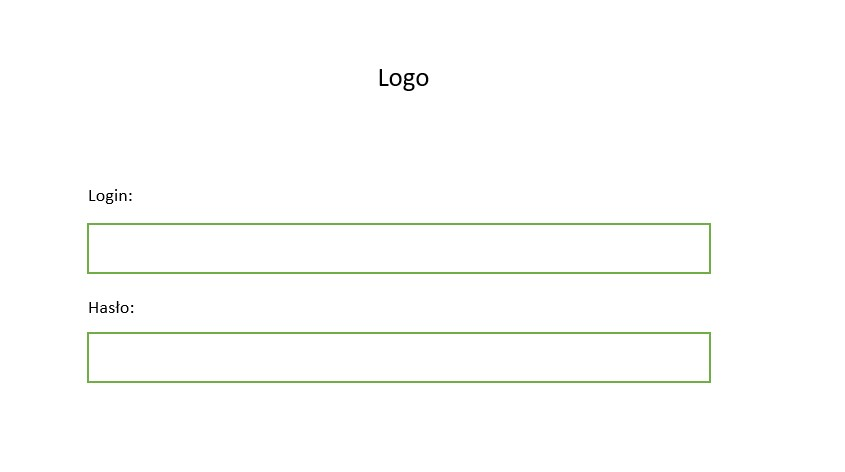
\includegraphics[angle=360, width=0.80\textwidth]{rys/Layout_2.jpg}
		\caption{Przykładowy panel logowania }
		\label{rys:Login}
	\end{center}
\end{figure}
\newpage
 Poniżej na rysunku 1.3 przedstawiamy wstępny layout aplikacji na jakim nam zależy, jeżeli chodzi o przyciski to zależałoby nam na tym aby zamiast wpisanych nazwy tak jak zostało to zaprojektowane na wstępnym layoucie pojawiły się ikonki przedstawiające daną funkcje; na przykład zamiast napisu "Latarka", pojawi się przycisk z wizerunkiem przedstawiającym latarkę; sprawi to że aplikacja będzie wyglądać jeszcze bardziej przejrzyście. \newline
 
 \begin{figure}[!hbt]
 	\begin{center}
 		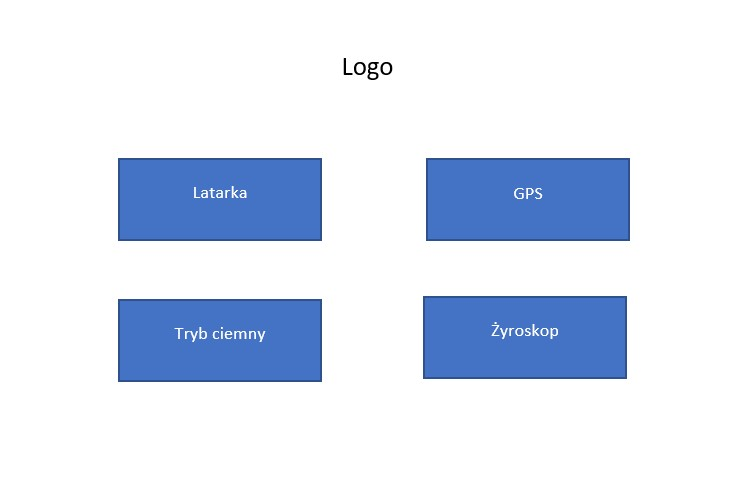
\includegraphics[angle=360, width=0.80\textwidth]{rys/Layout_1.jpg}
 		\caption{Przykładowy layout}
 		\label{rys:Layout}
 	\end{center}
 \end{figure}


  


 
 
 
 
 
   \newpage
\section{Określenie wymagań szczegółowych}		%2
%Dokładne określenie wymagań aplikacji (cel, zakres, dane wejściowe) – np. opisać przyciski, czujniki, wygląd layoutu, wyświetlenie okienek. Opisać zachowanie aplikacji – co po kliknięciu, zdarzenia automatyczne. Opisać możliwość dalszego rozwoju oprogramowania. Opisać zachowania aplikacji w niepożądanych sytuacjach.

\hspace{0.60cm}Firma nie związana z technologia pragnie aby stworzyć aplikację mobilną do testowania czujników, która byłaby  zachowana w sposób minimalistyczny i intuicyjny. Przejrzysta i prosta budowa menu, która miałaby na celu usprawnić szukanie odpowiednich komponentów. Firma posiada również logo, które powinno zawierać się w projekcie, jak i niebieskie akcenty (np. przyciski) - który jest przewodnim kolorem firmy. \newline

Jednym z kluczowych zadań jest stworzenie aplikacji w sposób jak najbardziej przejrzysty, do tego celu użyjemy ikonek, które w prosty i szybki sposób nakierują nas na odpowiedni komponent. Przykładem może być latarka; chcąc przetestować jej działanie wystarczy wybrać ikonkę która będzie przedstawiała latarkę. Po jej naciśnięciu zostaniemy przekierowani do strony z testem, który będzie posiadał dwa przyciski jeden to zielony włącznik oraz czerwony wyłącznik. Ponadto będziemy starać się aby wyniki testów były stopniowo zapisywane w pliku wyjściowym. Jako wykonawcy aplikacji chcielibyśmy wdrożyć do projektu przyciski które znajdowałyby się przy każdym teście i informowałyby o tym ,że: "test przebiegł pomyślnie" lub "test nie powiódł się". W zależnie od tego który przycisk naciśniemy to w taki sposób uzupełni się plik wyjściowy z podsumowaniem testu. Zapewniamy również zawarcie logotypu i motywu niebieskiego aplikacji, i sprawimy by layout w całości był jak najbardziej intuicyjny i zachowany w minimalistyczny sposób (brak jaskrawych kolorów, duże przejrzyste przyciski, okienka pop-up z wiadomościami o przebiegu testu). Postaramy się aby komponenty testujące takie jak: latarka, test dźwięku, czujnik światła, tryb nocny i tym podobne; będą poprawnie spełniać swoje zadanie. Aplikacja zostanie napisana w programie Android Studio, natomiast język którym będziemy się posługiwać to: Java. \newline

Tak jak już wspomnieliśmy powyżej postaramy się by każdy z czujników działał w należyty sposób; to znaczy by latarka poprzez kliknięcie przycisków włączała się i wyłączała. Test dźwięku pozwoli nam poprzez kliknięcie przycisku usłyszeć z głośników wydobywającą się melodię; tryb nocny, który jest bardzo przydatną funkcją w telefonie szczególnie wieczorami gdy korzystamy z urządzeń mobilnych, zmieni kolorystykę z jasnej na ciemną. Przez tą funkcję jaka jest tryb ciemny nasze oczy nie są narażane na tak mocne światło, co sprawia, że czujemy większy komfort w użytkowaniu telefonów komórkowych. Niektóre osoby preferują korzystanie z trybu nocnego nawet podczas dnia a nie tylko nocą. Kolejny czujnik jakim będzie GPS pozwoli nam w szybki sposób określić położenie w którym się znajdujemy. Test Wifi umożliwi spawdzenie połączenia z siecią, natomiast test mikrofonu sprawdzi się w sytuacji gdy na przykład pojawi się problem podczas rozmów telefonicznych. Test aparatu pozwoli wykonać zdjęcie oraz przetestować jakość wykonanego zdjęcia.  \newline
Pragnieniem firmy, która zleciła nam wykonanie aplikacji, jest stworzenie panelu logowania, dzięki któremu pracownicy wraz z klientami będą mogli logować się do aplikacji. Naszym zdaniem nie ma konieczności do tworzenia odrębnego panelu do logowania, ponieważ aplikacja wykonuje tylko testy czujników i nie przechowuję poufnych danych. Co więcej w sytuacji gdy kilkaset osób postanowi wejść w aplikację i zalogować się na nią, może dojść do przeciążenia i zawieszenia się strony, co wiążę się z tym, że nabywcy aplikacji będą musieli poczekać dłuższą chwilę aby logowanie się powiodło. Uważamy, że w dużych firmach mogłoby to spowolnić pracę pracowników, a czas pracy odgrywa bardzo ważną rolę.\newline

Rozpoczęliśmy pracę przy tworzeniu wstępnego layout strony głównej (rysunek 2.1) i na ten moment prezentuję się ona następująco: \newline 
 \begin{figure}[!hbt]
	\begin{center}
		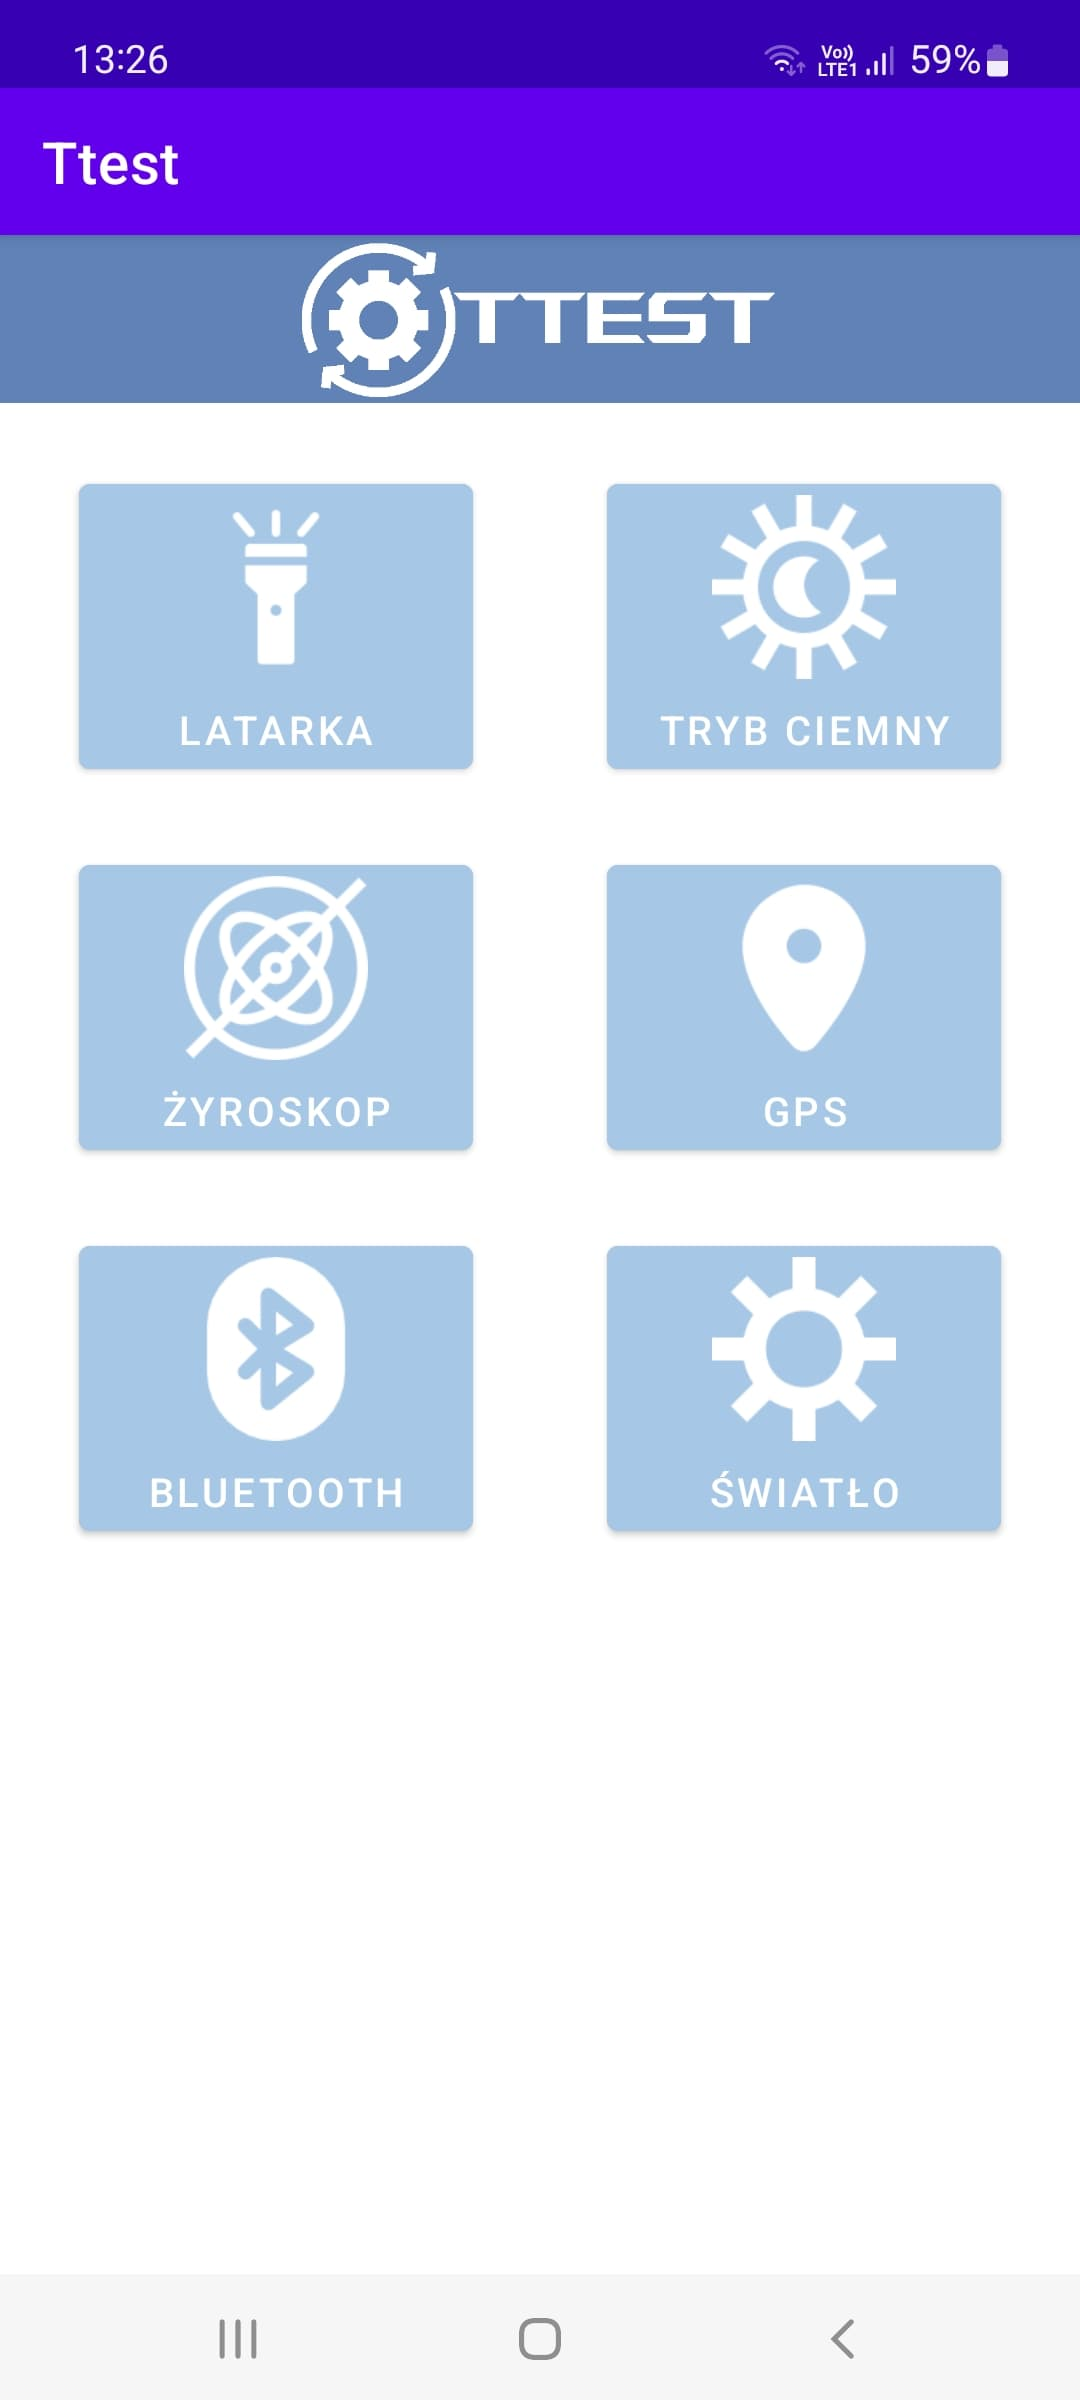
\includegraphics[angle=360, width=0.31\textwidth]{rys/menu.jpg}
		\caption{Wstępne menu}
		\label{rys:Menu}
	\end{center}
\end{figure}
\newpage
Na tą chwilę udało nam się stworzyć menu z sześcioma przyciskami, które prezentują poszczególne czujniki. Aktualnie przyciski nie przekierowują jeszcze na stronę testów lecz tym zajmiemy się w kolejnym etapie naszej pracy. Co więcej na górze ekranu dokładniej w jego centrum umieszczone zostało logo firmy, które dostaliśmy w zleceniu. Kolorystyka jest utrzymana w błękicie oraz bieli. 


   \newpage
\section{Projektowanie}		%3
%Opis przygotowania narzędzi (git, visual studio). Wybór i opis bibliotek, klas. Szkic layoutów. Pseudo kody. Opisy wykorzystanych algorytmów (np. algorytm sortowania). Dokładniejsze określenie założeń i działania aplikacji, (np.: ten przycisk otworzy takie okno a w tym oknie wpisujemy takie dane).
\subsection{Kilka słów o środowisku Android studio oraz języku programowania Java.}
\hspace{0.60cm}Android Studio to środowisko programistyczne (IDE) stworzone przez Google na bazie IntelliJ, które kierowane jest do developerów aplikacji na Androida. Pozwala ono wygodnie projektować, tworzyć i debugować własne programy na najpopularniejszą obecnie platformę systemową dla urządzeń mobilnych. Oprogramowanie oferuje podobne możliwości co środowisko Eclipse z zainstalowaną wtyczką ADT, jednak jest ono znacznie prostsze i bardziej intuicyjne w szczególności dla początkujących programistów. Przejęło ono wszystkie najlepsze rozwiązania znane użytkownikom IntelliJ, oferując narzędzie zoptymalizowane w dużym stopniu do wygodnej pracy z kodem źródłowym. Decydując się na korzystanie z Android Studio użytkownik otrzymuje środowisko programistyczne z przejrzystym i konfigurowalnym interfejsem graficznym, nie wspominając o funkcji kolorowania składni czy mechanizmie zakładek, pozwalającym na pracę z wieloma plikami jednocześnie. \newline

Java to wysokopoziomowy język programowania najczęściej wykorzystywany do tworzenia backendu aplikacji internetowych. Język ten jest łatwo przenośny, dzięki interpretowaniu przez wieloplatformową maszynę wirtualną Java Virtual Machine. Można stwierdzić, że Java jest językiem preferowanym przez korporacje i duże firmy. W Javie napisano m.in. takie aplikacje jak Gmail, OpenOffice czy Minecraft, ale także LinkedIn, Netflix czy Amazon.


\subsection{Środowisko programisty/Składanie dokumentów - Latex}
\hspace{0.60cm}Latex służy do wytwarzania przejrzyście wyglądających dokumentów tekstowych takich jak książki, artykuły, czy nawet prezentacje. Docelowym formatem jest wydruk, czy też pliki w różnych formatach, takich jak PDF, Postscript, czy też HTML. Szczególnie wygodne jest tworzenie dokumentów technicznych, matematycznych, ale z powodzeniem może też być stosowany do pisania dokumentacji programów albo zbioru opowiadań.\newline

Latex, podobnie jak języki programowania, ma swój własny język, w którym pisze się treść dokumentu oraz posiada narzędzia (można by powiedzieć "kompilatory"), które przetwarzają pliki źródłowe i generują pliki docelowe. W językach programowania zazwyczaj jedną z istotnych rzeczy jest zbiór bibliotek z gotowymi implementacjami różnych typowych czynności. Również w Latexu jest dużo gotowych pakietów pozwalających w szybki sposób tworzyć najróżniejsze elementy i rodzaje dokumentów.\newline

Filozofia Latexa jest taka, aby skupiać się na tym co merytorycznie ma zawierać dany dokument, a jak najmniej poświęcać uwagi na to, jak ma to wyglądać. Innymi słowy wprowadzamy tylko strukturę i zawartość dokumentu, a latex za nas robi resztę roboty, aby wyjściowy dokument wyglądał jak należy. Oczywiście mamy dużą możliwość ingerencji w wygląd, ale zazwyczaj jest to tylko dobieranie jakiegoś szablonu lub potrzeba uzyskania niestandardowego efektu. Jest to zupełnie inna filozofia, niż w wielu innych edytorach tekstowych, szczególnie w różnych aplikacjach biurowych, gdzie prawie na każdym kroku musimy od decydować, jaki ma być wygląd, wielkość liter, czcionka, odstępy, sposób wyświetlania tytułów itp.\newline 
Podstawą możliwości cieszenia się twórczością w Latexu jest posiadanie wszystkich narzędzi, pakietów, czcionek, itp. Gotowe zbiory są dostępne w różnych dystrybucjach. Oprócz tych narzędzi, początkujący użytkownicy mogą skorzystać z gotowych środowisk do obrabiania dokumentów Latexu.\newline
Podstawową dystrybucją jest TeX Live. Jest ona dostępna pod wiele różnych platform. Jest łatwą w instalacji kompletną paczką narzędzi, programów, czcionek.


\subsection{Czym jest Git oraz do czego służy?}
\hspace{0.60cm}Co to jest Git i dlaczego cieszy się tak dużą popularnością? Ten system kontroli wersji znacznie usprawnia, a jednocześnie zabezpiecza codzienną pracę przy kodzie. Dzięki swojej prostocie i elastyczności może być wykorzystywany zarówno przy drobnych, jak i ogromnych projektach. Dlatego też jest używany przez programistów oraz grafików na całym świecie. Odpowiadając w skrócie na pytanie, co to jest Git, należy powiedzieć, że to system kontroli wersji. Służy on więc do zarządzania historią kodu źródłowego. Jego funkcjonalność ma kilka podłoży. Między innymi sprawdza się tak dobrze, ponieważ\newline
- pozwala na jednoczesną pracę na tym samym kodzie przez kilka osób, \newline
- umożliwia transferowanie i łączenie zmian z różnych branchy w jednym projekcie\newline
- pozwala na pracę offline we własnym repozytorium \newline
- jest szybki i wydajny.\newline 
Cechy te sprawiły, że Git szybko został doceniony w całej branży. Przechowywanie wersji, a także możliwość rozgałęziania kodu to niewątpliwie jego ogromne zalety. 
\newline

GitHub z kolei to firma, która hostuje repozytoria Git i dostarcza oprogramowanie do korzystania z niego. Jednym z przykładów jest tytułowy GitHub Desktop na systemy Windows 10 i 11. GitHub jest obecnie najpopularniejszym hostem projektów open source pod względem zarówno liczby projektów , jak i użytkowników. Choć GitHub koncentruje się głównie na kodzie źródłowym, to inne projekty coraz częściej wykorzystują systemy kontrolowania wersji do zarządzania przepływem pracy związanym z publikowaniem czasopism, artykułów, podręczników itp.\newline

Test rozpoczynamy od uruchomienia naszej aplikacji a następnie pojawia nam się główne menu (rysunek 3.1), które składa się z dużych przycisków, zachowanych w kolorystyce firmy.
Na każdym z przycisków widnieje ikonka przedstawiającą daną funkcję na przykład: chcemy przetestować latarkę; klikamy przycisk, który ją przedstawia.\newline
%rysunek
\begin{figure}[!hbt]
	\begin{center}
		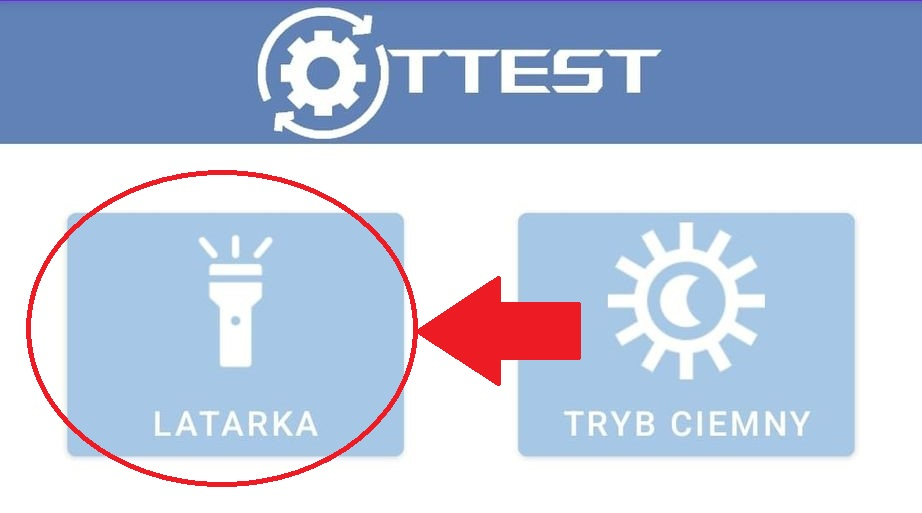
\includegraphics[angle=360, width=0.80\textwidth]{rys/przyklad_1.jpg}
		\caption{Przykładowy przycisk}
		\label{rys:przyklad}
	\end{center}
\end{figure}
\newline

Po kliknięciu ikonki, aplikacja przekierowuje nas do testu (rysunek 3.2), gdzie pojawiają się dwie latarki w centralnej części ekranu: po lewej stronie w kolorze zielonym a po prawej stronię w czerwonym. Kolor zielony ma na celu informować nas o tym że latarka jest włączona i działa, natomiast kolor czerwony sygnalizuje, że latarka jest wyłączona.
\newpage
%rysunek
\begin{figure}[!hbt]
	\begin{center}
		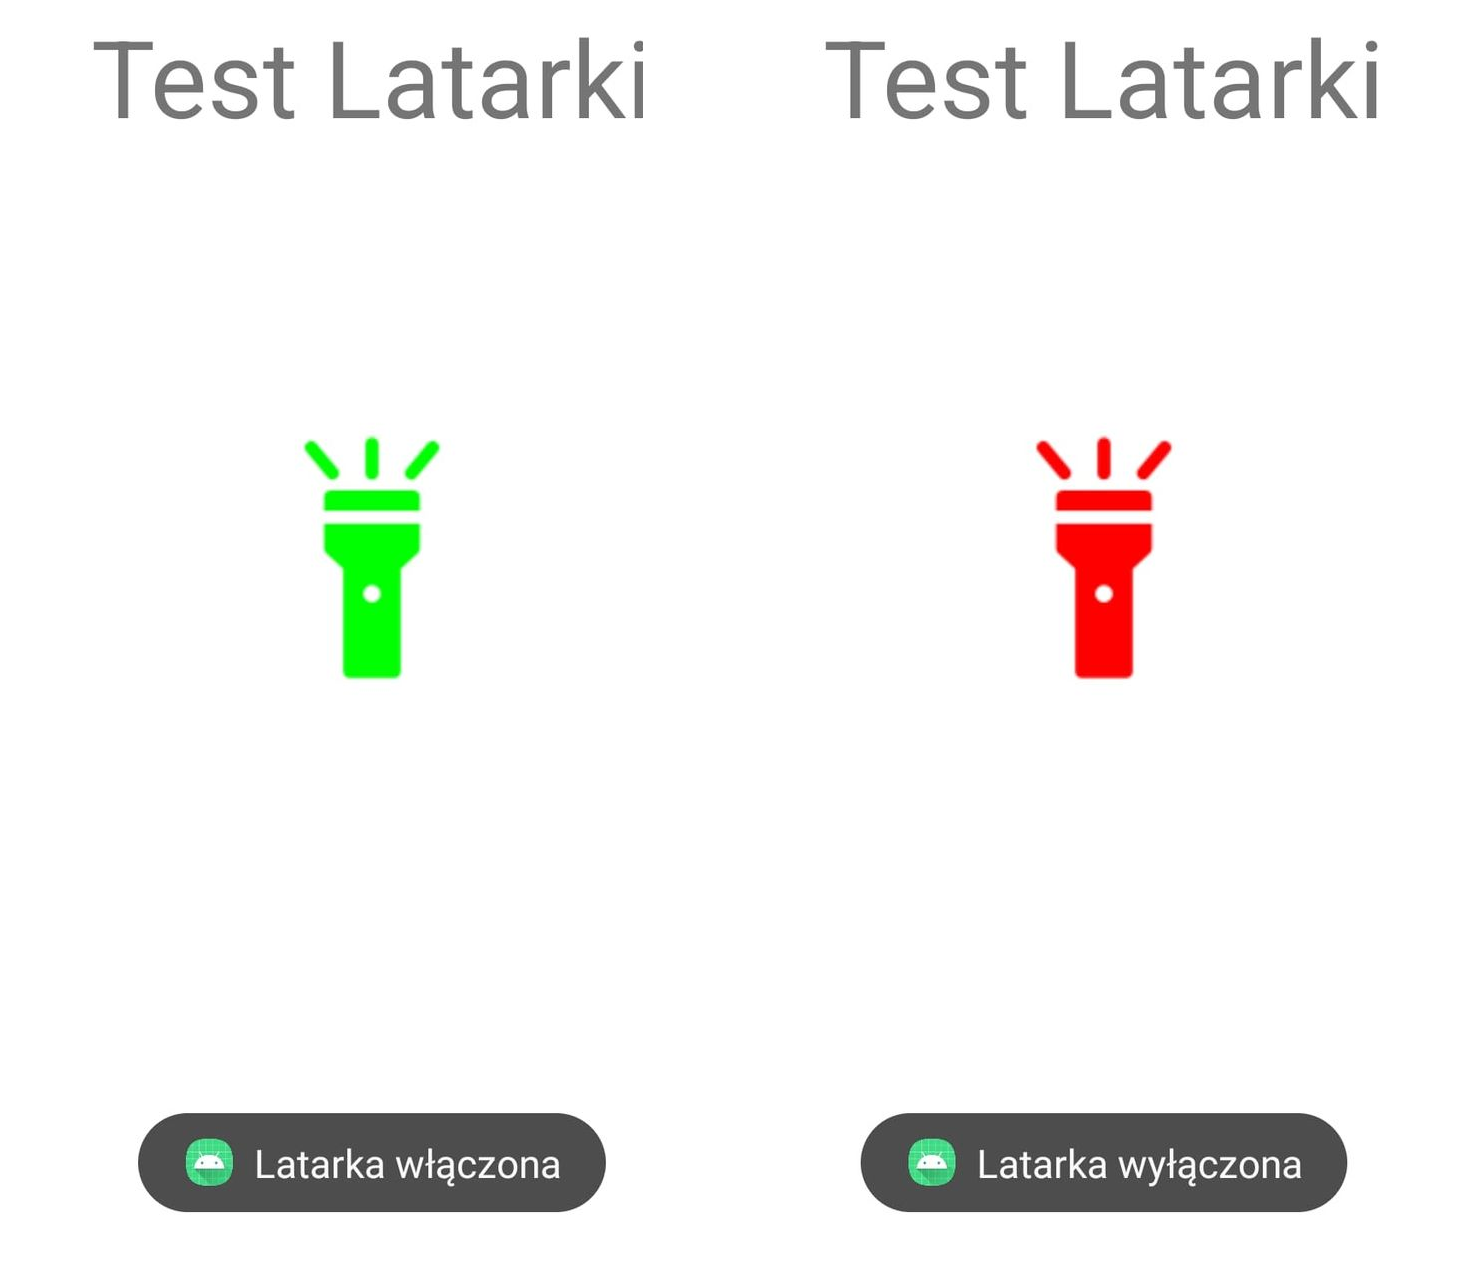
\includegraphics[angle=360, width=0.70\textwidth]{rys/przyklad_2.png}
		\caption{Test latarki}
		\label{rys:przyklad}
	\end{center}
\end{figure}   



   	\newpage
\section{Implementacja}		%4


Listing \ref{lst:listing-java} (s. \pageref{lst:listing-java}) przedstawia implementacje jednego z przycisków którego zadaniem jest otworzenie nowej strony oznaczonej w 5 linijce kodu po kliknięciu. 
\begin{lstlisting}[caption=Menu - Działanie Przycisków, label={lst:listing-java}, language=Java]
	button_1 = (Button) findViewById(R.id.button_1);
	button_1.setOnClickListener(new View.OnClickListener() {
		@Override
		public void onClick(View view) {
			Intent intent = new Intent(MainActivity.this, latarka.class);
			startActivity(intent);
		}
	});
\end{lstlisting}


Listing \ref{lst:listing-java2} (s. \pageref{lst:listing-java2}) przedstawia włączenie latarki. Jeśli telefon ma latarkę i mamy do niej dostęp, latarka zostanie uruchomiona i wyświetli się nam komunikat o włączeniu. Jeżeli nie, to dostaniemy odpowiednie powiadomienie o niepowodzeniu operacji. \\
W podobny sposób wygląda metoda z wyłączeniem latarki. W 6 linijce trzeba zamienić wartość na false oraz w 7 wierszu nadpisać wyświetlany komunikat na odpowiedni.
\begin{lstlisting}[caption=Latarka - Włączenie/wyłączenie latarki, label={lst:listing-java2}, language=Java]
	private void flashLightOn(){
		CameraManager cameraManager = (CameraManager) getSystemService(Context.CAMERA_SERVICE);
		try{
			assert cameraManager != null;
			String cameraId = cameraManager.getCameraIdList()[0];
			cameraManager.setTorchMode(cameraId, true);
			Toast.makeText(latarka.this, "Latarka wlaczona", Toast.LENGTH_SHORT).show();
		}
		catch(CameraAccessException e){
			Log.e("Camera Problem", "Nie mozna uruchomic latarki");
		}
	}
\end{lstlisting}

\newpage


Aby zaimplementować tryb ciemny potrzebujemy dostępu do modyfikowania interfejsu. Listing \ref{lst:listing-java3} (s. \pageref{lst:listing-java3}) pokazuje jak go uzyskać. 
\begin{lstlisting}[caption=Tryb Ciemny - Modyfikowanie interfejsu, label={lst:listing-java3}, language=Java]
	SharedPreferences sharedPreferences = getSharedPreferences("sharedPrefs", MODE_PRIVATE);
	final SharedPreferences.Editor editor = sharedPreferences.edit();
	final boolean isDarkModeOn = sharedPreferences.getBoolean("isDarkModeOn", false);
\end{lstlisting}


 Listing \ref{lst:listing-java4} (s. \pageref{lst:listing-java4}) przedstawia metodę odpowiedzialną za działanie trybu ciemnego. Domyślnie aplikacja korzysta z trybu jansego, co pokazuje kod od 5 do 10 linijki. Jednak po naciśnięciu na przycisku, zmieniamy kolorystyke aplikacji na ciemną (13-15 linijak), dodatkowo od 16 linijki zmieniamy przycisk na czerwony, aktualne logo na ciemne oraz wyświetlamy stosowny komunikat.
\begin{lstlisting}[caption=Tryb Ciemny - Włączenie/wyłączenie trybu ciemnego, label={lst:listing-java4}, language=Java]
	toggle_tryb_ciemny.setOnClickListener(new View.OnClickListener() {
		@Override
		public void onClick(View view) {
			if(isDarkModeOn){
				AppCompatDelegate.setDefaultNightMode(AppCompatDelegate.MODE_NIGHT_NO);
				editor.putBoolean("isDarkModeOn", false);
				editor.apply();
				toggle_tryb_ciemny.setImageResource(R.drawable.tryb_ciemny_off);
				logo.setImageResource(R.drawable.logo_white);
				Toast.makeText(tryb_ciemny.this, "Tryb ciemny wylaczony", Toast.LENGTH_SHORT).show();
			}
			else {
				AppCompatDelegate.setDefaultNightMode(AppCompatDelegate.MODE_NIGHT_YES);
				editor.putBoolean("isDarkModeOn", true);
				editor.apply();
				toggle_tryb_ciemny.setImageResource(R.drawable.tryb_ciemny_on);
				logo.setImageResource(R.drawable.logo_black);
				Toast.makeText(tryb_ciemny.this, "Tryb ciemny wlaczony", Toast.LENGTH_SHORT).show();
			}
		}
	});
\end{lstlisting}

\newpage


Listing \ref{lst:listing-java5} (s. \pageref{lst:listing-java5}) prezentuje uzyskanie dostępu do sensora, za pomocą którego sprawdzimy działanie czujnika zbliżeniowego.
\begin{lstlisting}[caption=Czujnik Zbliżeniowy - Dostęp do czujnika, label={lst:listing-java5}, language=Java]
	SensorManager sensorManager;
	sensorManager = (SensorManager)getSystemService(SENSOR_SERVICE);
	if(sensorManager!=null) {
		Sensor proximitySensor = sensorManager.getDefaultSensor(Sensor.TYPE_PROXIMITY);
		if(proximitySensor!=null) {
			sensorManager.registerListener(this, proximitySensor, sensorManager.SENSOR_DELAY_NORMAL);
		}
	}
\end{lstlisting}


Metoda onSensorChanged ukazana na listingu \ref{lst:listing-java6} (s. \pageref{lst:listing-java6}) sprawdza czy przy czujniku jest obiekt, zależnie od wyniku zostanie wyświetlony odpowiedni komunikat.
\begin{lstlisting}[caption=Czujnik Zbliżeniowy - Działanie, label={lst:listing-java6}, language=Java]
	@Override
	public void onSensorChanged(SensorEvent sensorEvent) {
		if(sensorEvent.sensor.getType()==Sensor.TYPE_PROXIMITY) {
			if(sensorEvent.values[0]==0) {
				((TextView)findViewById(R.id.sensor)).setText("Przy czujniku jest obiekt");
			} else {
				((TextView)findViewById(R.id.sensor)).setText("Przyloz obiekt do czujnika");
			}
		}
	}
\end{lstlisting}


Aby wdrożyć test aplikacji trzeba sprawdzić pozwolenie, w tym wypadku interesuje nas uprawnienie dostępu do lokalizacji, co obrazuje listing  \ref{lst:listing-java7} (s. \pageref{lst:listing-java7}). 
\begin{lstlisting}[caption=GPS - Dostęp do lokazlizacji, label={lst:listing-java7}, language=Java]
	if(ContextCompat.checkSelfPermission(gps.this, Manifest.permission.ACCESS_FINE_LOCATION) != PackageManager.PERMISSION_GRANTED) {
		ActivityCompat.requestPermissions(gps.this, new String[]{
			Manifest.permission.ACCESS_FINE_LOCATION
		}, 1000);
	}
\end{lstlisting}

\newpage


Metoda onLocationChanged przedstawiona jako listing \ref{lst:listing-java8} (s. \pageref{lst:listing-java8}) odpowiada za wyświetlenie powiadomienia push-up wyświetlającego długość i szerokość geograficzną obecnej lokalizacji oraz pobiera adres tej lokalizacji na podstawie długości i szerokości geograficznej, który wyświetla jako tekst.
\begin{lstlisting}[caption=GPS - Wyświetlanie lokalizacji, label={lst:listing-java8}, language=Java]
	@Override
	public void onLocationChanged(Location location) {
		Toast.makeText(this, ""+location.getLatitude()+", "+location.getLongitude(), Toast.LENGTH_SHORT).show();
		try {
			Geocoder geocoder = new Geocoder(gps.this, Locale.getDefault());
			List<Address> addresses = geocoder.getFromLocation(location.getLatitude(), location.getLongitude(), 1);
			String address = addresses.get(0).getAddressLine(0);
			text_location.setText(address);
		} catch (Exception e) {
			e.printStackTrace();
		}
	}
\end{lstlisting}


Listing \ref{lst:listing-java9} (s. \pageref{lst:listing-java9}) przedstawia implementacje MediaPlayer (linijka 1) do którego podłączamy dźwięk. Teraz w prosty sposób możemy wywołać dźwięk poprzez medote OnClick,
\begin{lstlisting}[caption= Dźwięk - Działanie z wykorzystaniem MediaPlayer, label={lst:listing-java9}, language=Java]
	final MediaPlayer sound = MediaPlayer.create(this, R.raw.dzwiek_audio);
	Button btn_dzwiek = findViewById(R.id.btn_dzwiek);
	btn_dzwiek.setOnClickListener(new View.OnClickListener() {
		@Override
		public void onClick(View view) {
			sound.start();
		}
	});
\end{lstlisting}

\newpage


Aby test mikrofonu spełniał swoje zadanie trzeba sprawdzić autoryzację aplikacji. W tym wypadku uzyskujemy pozwolenie na nagrywanie audio, co przedstawia listing \ref{lst:listing-java10} (s. \pageref{lst:listing-java10}). 
\begin{lstlisting}[caption=Mikrofon - Dostęp do nagrywania audio, label={lst:listing-java10}, language=Java]
	private void getMicrophonePermission() {
		if(ContextCompat.checkSelfPermission(this, Manifest.permission.RECORD_AUDIO) == PackageManager.PERMISSION_DENIED) {
			ActivityCompat.requestPermissions(this, new String[] {Manifest.permission.RECORD_AUDIO}, MICROPHONE_PERMISSION_CODE);
		}
	}
\end{lstlisting}


Listing \ref{lst:listing-java11} (s. \pageref{lst:listing-java11}) przedstawia metodę z wykorzystaniem MediaRecorder który służy do nagrywania dźwięku lub obrazu. W tym wypadku MediaRecorder wykorzystany zostanie do nagrania dźwięku przez mikrofon w telefonie. Od 4 do 7 linijki określamy źródło dźwięku, format wyjściowy, zaznaczenie deskryptora pliku, definiowanie kodowania dźwięku.
\begin{lstlisting}[caption=Mikrofon - Włączenie nagrywania, label={lst:listing-java11}, language=Java]
	public void btnRecordPressed(View v) {
		try {
			mediaRecorder = new MediaRecorder();
			mediaRecorder.setAudioSource(MediaRecorder.AudioSource.MIC);
			mediaRecorder.setOutputFormat(MediaRecorder.OutputFormat.THREE_GPP);
			mediaRecorder.setOutputFile(getRecordingFilePath());
			mediaRecorder.setAudioEncoder(MediaRecorder.AudioEncoder.AMR_NB);
			mediaRecorder.prepare();
			mediaRecorder.start();
			
			Toast.makeText(this, "Nagrywanie rozpoczete", Toast.LENGTH_LONG).show();
		}
		catch (Exception e) {
			e.printStackTrace();
	}
\end{lstlisting}
	
\newpage
	
	
Po naciśnięciu przycisku "Stop" nagranie zostaje zakończone, co obrazuje listing \ref{lst:listing-java12} (s. \pageref{lst:listing-java12}). MediaRecorder kończy nagrywanie, a opcja realse użyta w 3 linijce nie pozwoli na ponowne uruchomienie pliku dźwiękowego w celu dogrania do niego dźwięku.
\begin{lstlisting}[caption=Mikrofon - Przerwanie nagrywania, label={lst:listing-java12}, language=Java]
	public void btnStopPressed(View v) {
		mediaRecorder.stop();
		mediaRecorder.release();
		mediaRecorder = null;
			
		Toast.makeText(this, "Nagrywanie zakonczone", Toast.LENGTH_LONG).show();
	}
\end{lstlisting}
	
Obiekt MediaPlayer wykorzystany w listingu \ref{lst:listing-java13} (s. \pageref{lst:listing-java13}) służy do obsługi odtwarzania plików audio i wideo. W 4 linijce kodu określamy skąd ma zostać pobrany plik, a następnie plik z dźwiękiem zostanie włączony.
\begin{lstlisting}[caption=Mikrofon - Odtworzenie nagrania, label={lst:listing-java13}, language=Java]
	public void btnPlayPressed(View v) {
		try {
			mediaPlayer = new MediaPlayer();
			mediaPlayer.setDataSource(getRecordingFilePath());
			mediaPlayer.prepare();
			mediaPlayer.start();
				
			Toast.makeText(this, "Odtwarzanie nagrania", Toast.LENGTH_LONG).show();
		}
		catch(Exception e){
			e.printStackTrace();
		}
	}
\end{lstlisting}

\newpage

Metoda przedstawiona na listingu \ref{lst:listing-java14} (s. \pageref{lst:listing-java14}), odpowiada za uruchomienie aparatu w telefonie po naciśnięciu przycisku o id btnCam. Od 6 do 8 linijki znajduję się kod opowiedzialny za uruchomienie aplikacji aparatu.
\begin{lstlisting}[caption=Aparat - Włączenie aparatu, label={lst:listing-java14}, language=Java]
	btnCam = findViewById(R.id.btnCam);
	btnCam.setOnClickListener(new View.OnClickListener() {
		@Override
		public void onClick(View view) {
			try {
				Intent intent = new Intent();
				intent.setAction(MediaStore.ACTION_IMAGE_CAPTURE);
				startActivity(intent);
			} catch (Exception e) {
				e.printStackTrace();
			}
		}
	});
\end{lstlisting}

Pętla switch (rozpoczynająca się w linijce 6) przedstawiona w listingu \ref{lst:listing-java15} (s. \pageref{lst:listing-java15}) odpowiada za informowanie użytkowanika o aktualnym statusie wifi. W linijce 7 sprawdzamy czy Wifi jest włączone, jeśli jest włączone - wyświetlamy odpowiedni tekst, w 10 linijce sprawdzamy czy wifi jest wyłączone na danym urządzeniu, jeśli tak zostaje wyświetlony adekwatny tekst.
\begin{lstlisting}[caption=Wifi - Sprawdzenie statusu Wifi, label={lst:listing-java15}, language=Java]
	private BroadcastReceiver wifiStateReceiver = new BroadcastReceiver() {
		@Override
		public void onReceive(Context context, Intent intent) {
			int wifiStateExtra = intent.getIntExtra(WifiManager.EXTRA_WIFI_STATE,
			WifiManager.WIFI_STATE_UNKNOWN);
			switch (wifiStateExtra) {
				case WifiManager.WIFI_STATE_ENABLED:
				wifiSwitch.setText("WiFi jest wlaczone, mozna pobrac informacje");
				break;
				case WifiManager.WIFI_STATE_DISABLED:
				wifiSwitch.setText("WiFi jest wylaczone, wlacz aby pobrac informacje");
				break;
			}
		}
	};
\end{lstlisting}

\newpage

Metoda przedstawiona na listingu \ref{lst:listing-java16} (s. \pageref{lst:listing-java16}) odpowiada za pobranie informacji o sieci wifi do której urządzenie jest obecnie podłączone oraz wyświetlenia tych informacji. Od 5 do 9 linijki mamy kolejno pobranie informacji o adresie IP telefonu, sformatowanie pobranego IP ma tekst, pobranie adresu MAC routera, SSID oraz wskaźnika mocy naszego połączenia. Pobrane informacje implementujmey jako string (od 11 do 15 linijki) i wyświetlamy jako tekst (linijka 17).
\begin{lstlisting}[caption=Wifi - Pobieranie informacji o Wifi, label={lst:listing-java16}, language=Java]
    public void getWifiInformation(View view) {
	WifiManager wifiManager = (WifiManager) getApplicationContext().getSystemService(WIFI_SERVICE);
	WifiInfo wifiInfo = wifiManager.getConnectionInfo();
	
	int ip = wifiInfo.getIpAddress();
	String ipAddress = Formatter.formatIpAddress(ip);
	String bssid = wifiInfo.getBSSID();
	String ssid = wifiInfo.getSSID();
	int rssi = wifiInfo.getRssi();
		
	String info =
	"\n Adres IP: " + ipAddress +
	"\n Adres MAC Routera: " + bssid +
	"\n SSID: " + ssid +
	"\n Wskaznik mocy: " + rssi;
	txtWifiInfo.setText(info);	
}
\end{lstlisting}


Kod ukazany w listingu \ref{lst:listing-java17} (s. \pageref{lst:listing-java17}) jest odpowiedzialny za pobranie marki i modeu urządzenia z którego obecnie korzystamy i wyświetlenie tej informacji jako tekst.
\begin{lstlisting}[caption=Wyniki - Pobranie marki i modelu urządzenia, label={lst:listing-java17}, language=Java]
	model = (TextView) findViewById(R.id.model);
	String stringBuildModel = "Marka i model: " + Build.MANUFACTURER + " " + Build.MODEL;
	model.setText(stringBuildModel);
\end{lstlisting}



   	\newpage
\section{Testowanie}	%5
%Opisujemy testy, sprawdzamy czy nie generuje błędów.


\subsection{Testowanie latarki}

Zadania jakie ma spełniać test latarki przedstawione są w tabeli \ref{tab:tablica_latarka}. Jako "X" w kolumnie "Tak" lub "Nie", oznaczamy pomyślny lub niepomyślny przebieg poszczególnych zadań. Całość testu podsumowana jest rzutami ekranu \ref{rys:latarka} wykonanymi podczas testowania jako potwierdzenie wykonanego testu.

\begin{tabela}
	{Testowanie latarki}	%opis w spisie tabel
	{Testowanie latarki}	%opis przy tabeli
	{
		\begin{tabular}{|c|c|c|c|c|} \hline
			\textbf{lp} & \textbf{Zadania do przetestowania} & \textbf{Tak} & \textbf{Nie} \\ \hline
			1 & Latarka po naciśnięciu na guzik włączyła się & X & ~ \\ \hline
			2 & Po włączeniu latarki, guzik zmienia kolor na zielony & X & ~ \\ \hline
			3 & Wyświetlenie komunikatu o włączeniu latarki & X & ~ \\ \hline
			4 & Latarka po naciśnięciu na guzik wyłączyła się & X & ~ \\ \hline
			5 & Po wyłączeniu latarki, guzik zmienia kolor na czerwony & X & ~ \\ \hline
			6 & Wyświetlenie komunikatu o wyłączeniu latarki & X & ~ \\ \hline
		\end{tabular}	}
	\label{tab:tablica_latarka}
\end{tabela}

Obrazek \ref{rys:latarka} przedstawia zrzuty ekranu potwierdzające pomyślny przebieg testu.

\begin{figure}[!hbt]
	\begin{center}
		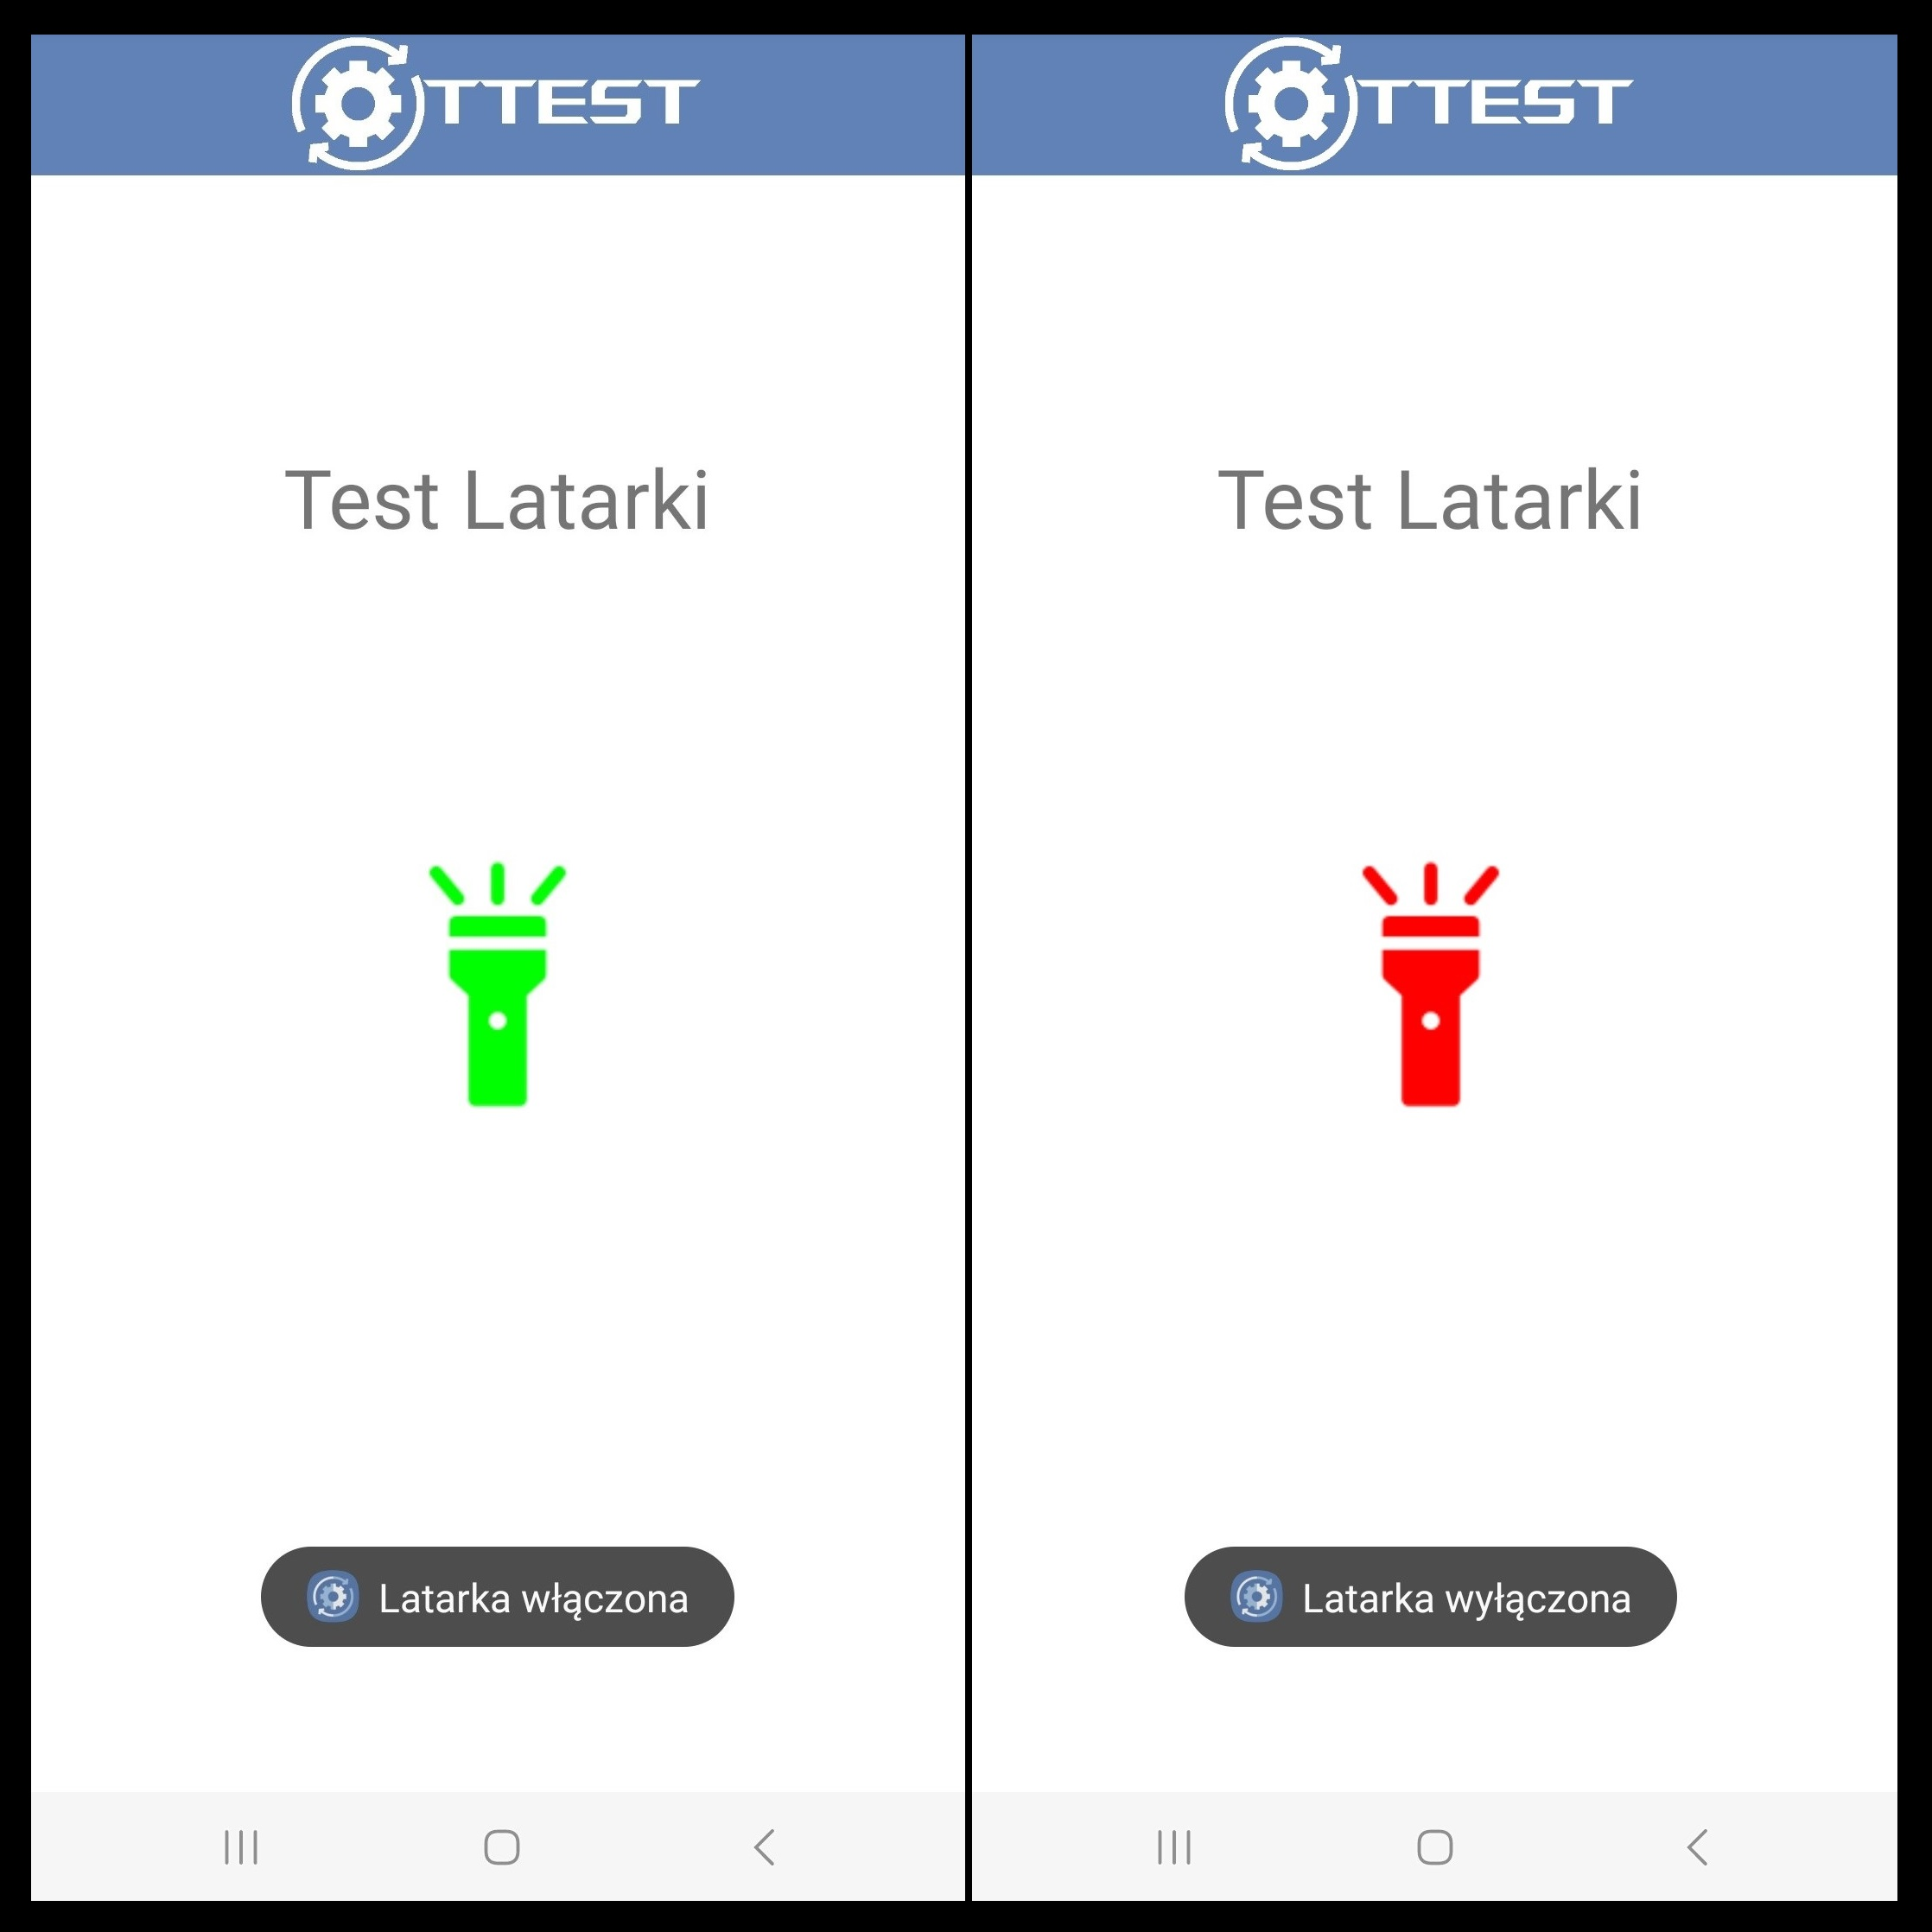
\includegraphics[angle=360, width=0.65\textwidth]{rys/punkt5/latarka.jpg}
		\caption{Przebieg testowania latarki}
		\label{rys:latarka}
	\end{center}
\end{figure}   

\newpage


\subsection{Testowanie trybu ciemnego}

Zadania jakie ma spełniać test trybu ciemnego przedstawione są w tabeli \ref{tab:tablica_ciemny}. Jako "X" w kolumnie "Tak" lub "Nie", oznaczamy pomyślny lub niepomyślny przebieg poszczególnych zadań. Całość testu podsumowana jest rzutami ekranu \ref{rys:ciemny} wykonanymi podczas testowania jako potwierdzenie wykonanego testu.

\begin{tabela}
	{Testowanie trybu ciemnego}	%opis w spisie tabel
	{Testowanie trybu ciemnego}	%opis przy tabeli
	{
		\begin{tabular}{|c|c|c|c|c|} \hline
			\textbf{lp} & \textbf{Zadania do przetestowania} & \textbf{Tak} & \textbf{Nie} \\ \hline
			1 & Tryb ciemny po naciśnięciu na guzik włączył się & X & ~ \\ \hline
			2 & Po włączeniu trybu ciemnego, guzik zmienia kolor na zielony & X & ~ \\ \hline
			3 & Wyświetlenie komunikatu o włączeniu trybu ciemnego & X & ~ \\ \hline
			4 & Tryb ciemny po naciśnięciu na guzik wyłączył się & X & ~ \\ \hline
			5 & Po wyłączeniu trybu ciemnego, guzik zmienia kolor na czerwony & X & ~ \\ \hline
			6 & Wyświetlenie komunikatu o wyłączeniu trybu ciemnego & X & ~ \\ \hline
	\end{tabular}	}
	\label{tab:tablica_ciemny}
\end{tabela}

Obrazek \ref{rys:ciemny} przedstawia zrzuty ekranu potwierdzające pomyślny przebieg testu.

\begin{figure}[!hbt]
	\begin{center}
		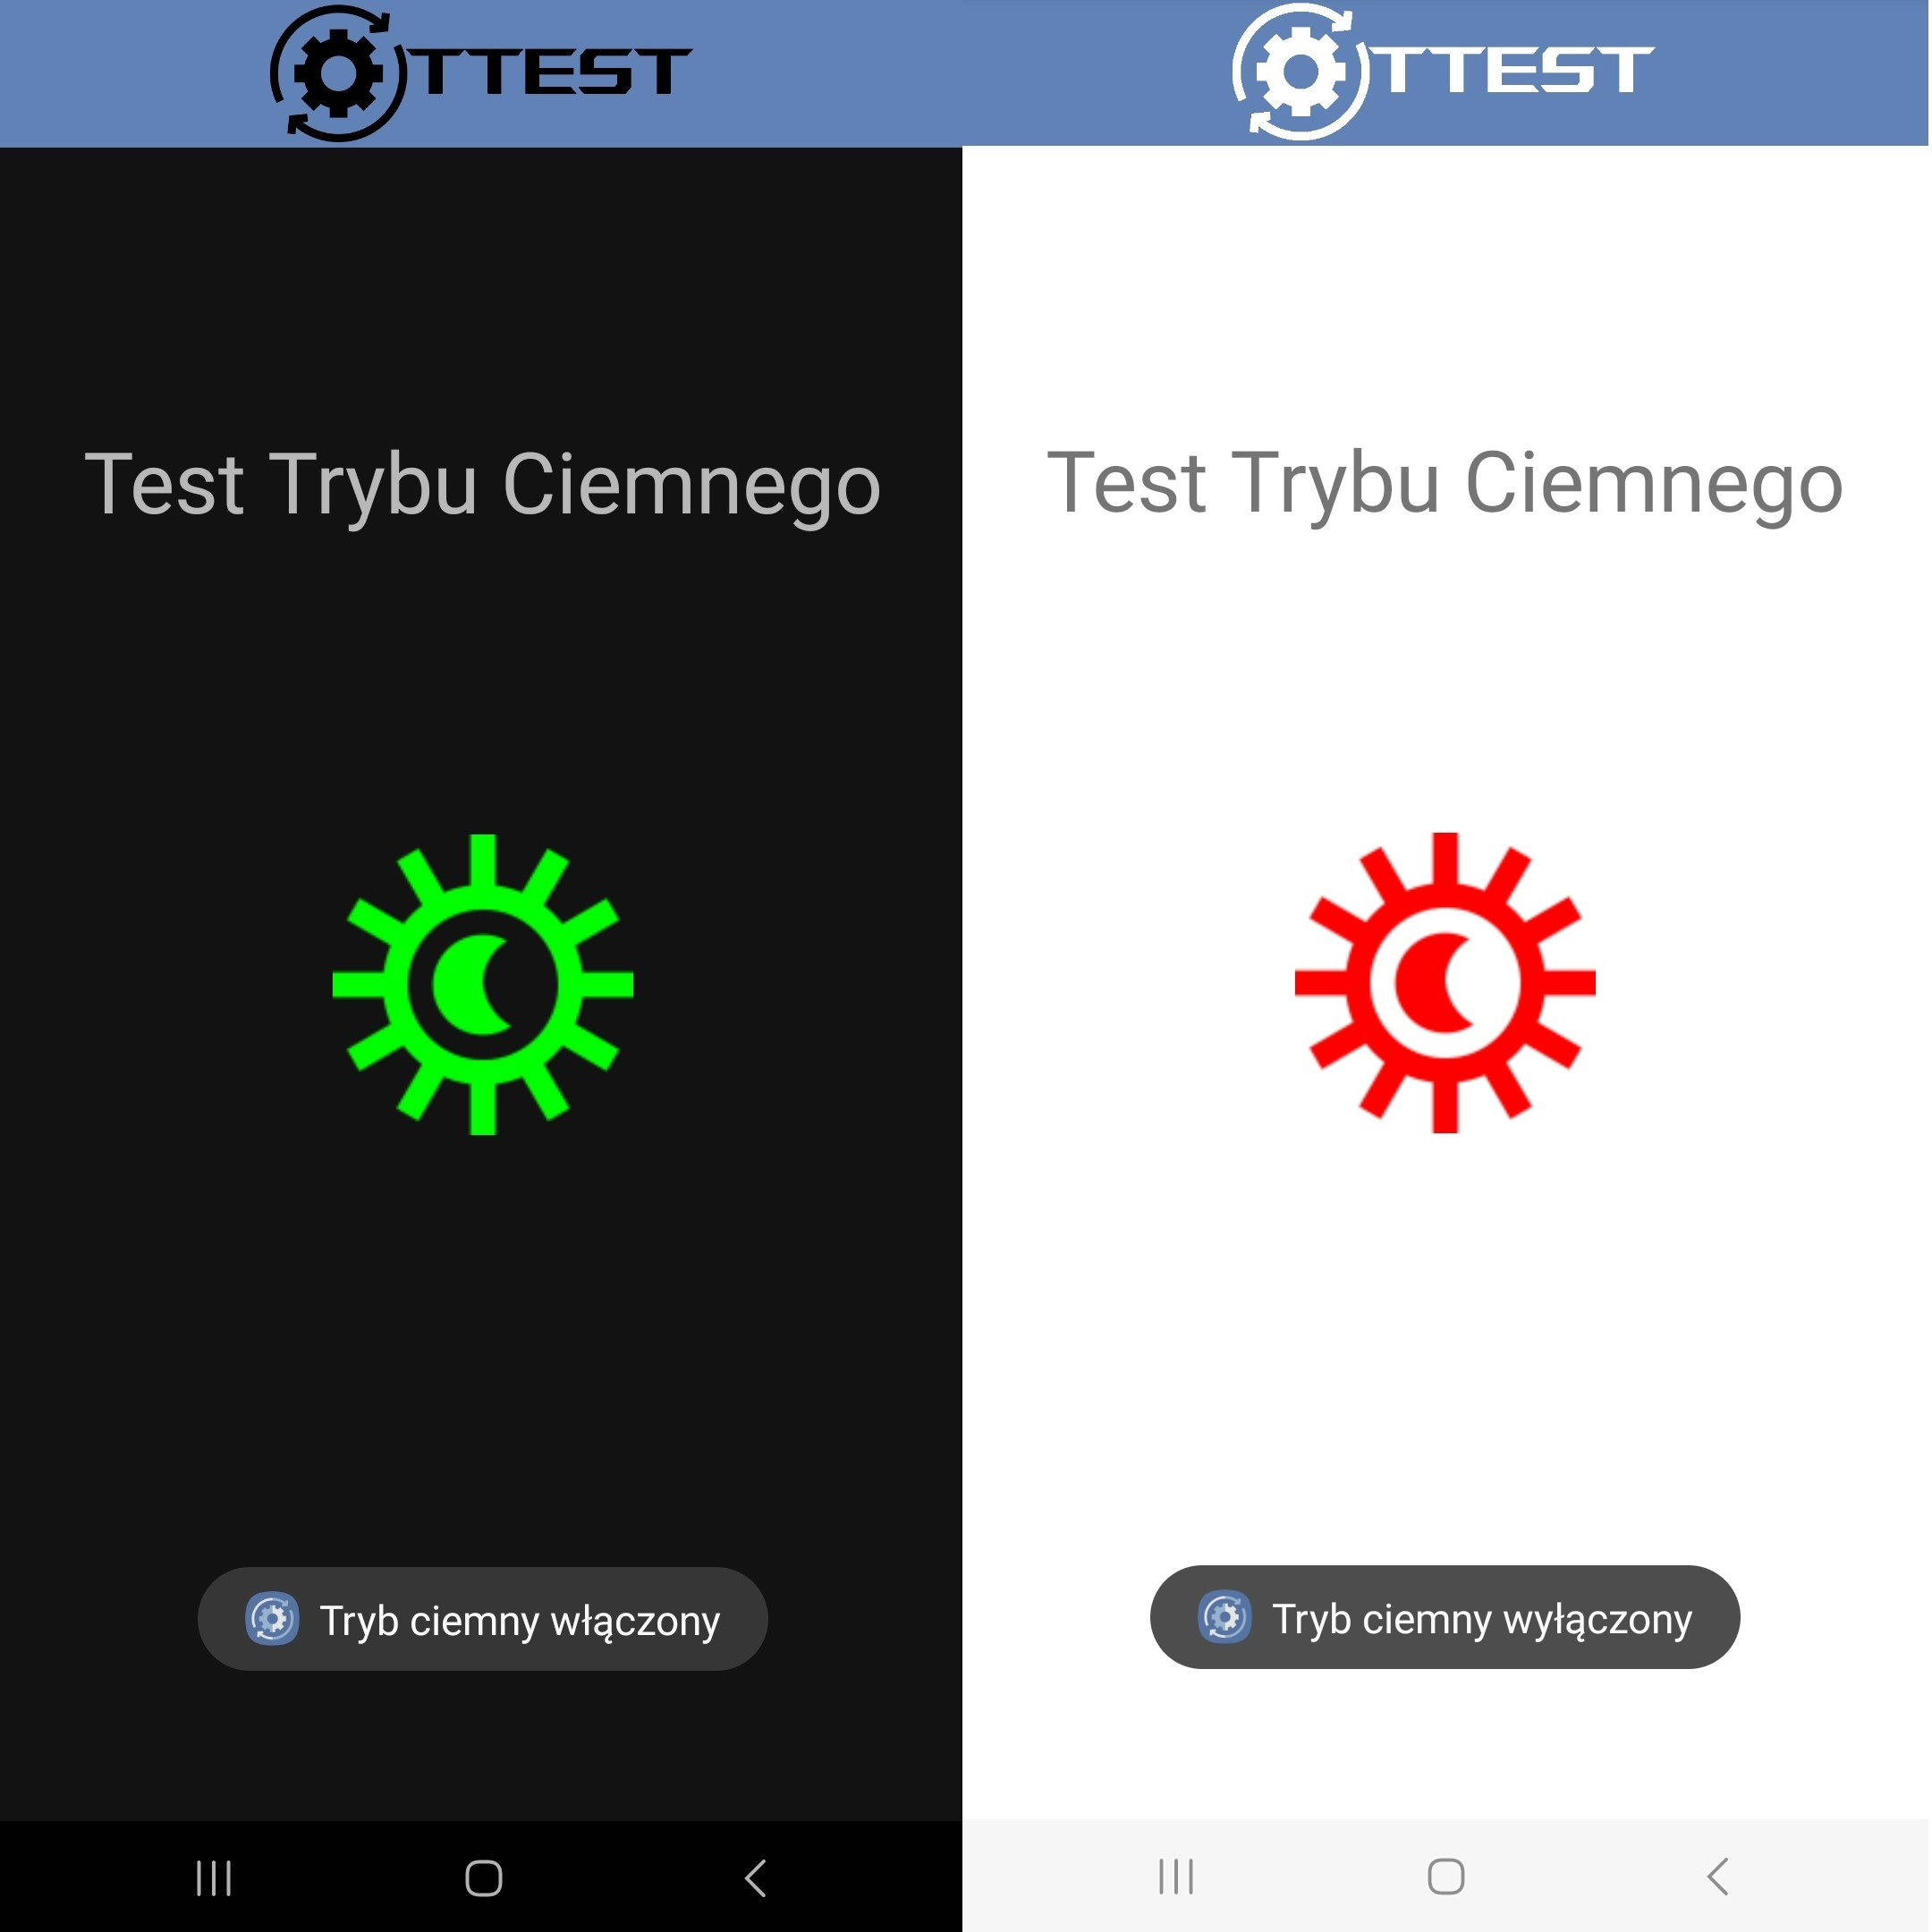
\includegraphics[angle=360, width=0.65\textwidth]{rys/punkt5/ciemny.jpg}
		\caption{Przebieg testowania trybu ciemnego}
		\label{rys:ciemny}
	\end{center}
\end{figure}   

\newpage


\subsection{Testowanie czujnika zbliżeniowego}

Zadania jakie ma spełniać test czujnika zbliżeniiowego przedstawione są w tabeli \ref{tab:tablica_zblizeniowy}. Jako "X" w kolumnie "Tak" lub "Nie", oznaczamy pomyślny lub niepomyślny przebieg poszczególnych zadań. Całość testu podsumowana jest rzutami ekranu \ref{rys:zblizeniowy} wykonanymi podczas testowania jako potwierdzenie wykonanego testu.

\begin{tabela}
	{Testowanie czujnika zbliżeniowego}	%opis w spisie tabel
	{Testowanie czujnika zbliżeniowego}	%opis przy tabeli
	{
		\begin{tabular}{|c|c|c|c|c|} \hline
			\textbf{lp} & \textbf{Zadania do przetestowania} & \textbf{Tak} & \textbf{Nie} \\ \hline
			1 & Po zbiżeniu obiektu do czujnik zmienia się tekst informacyjny  & X & ~ \\ \hline
			2 & Po oddaleniu obiektu od czujnika zmienia się tekst informacyjny & X & ~ \\ \hline
	\end{tabular}	}
	\label{tab:tablica_zblizeniowy}
\end{tabela}

Obrazek \ref{rys:zblizeniowy} przedstawia zrzuty ekranu potwierdzające pomyślny przebieg testu.

\begin{figure}[!hbt]
	\begin{center}
		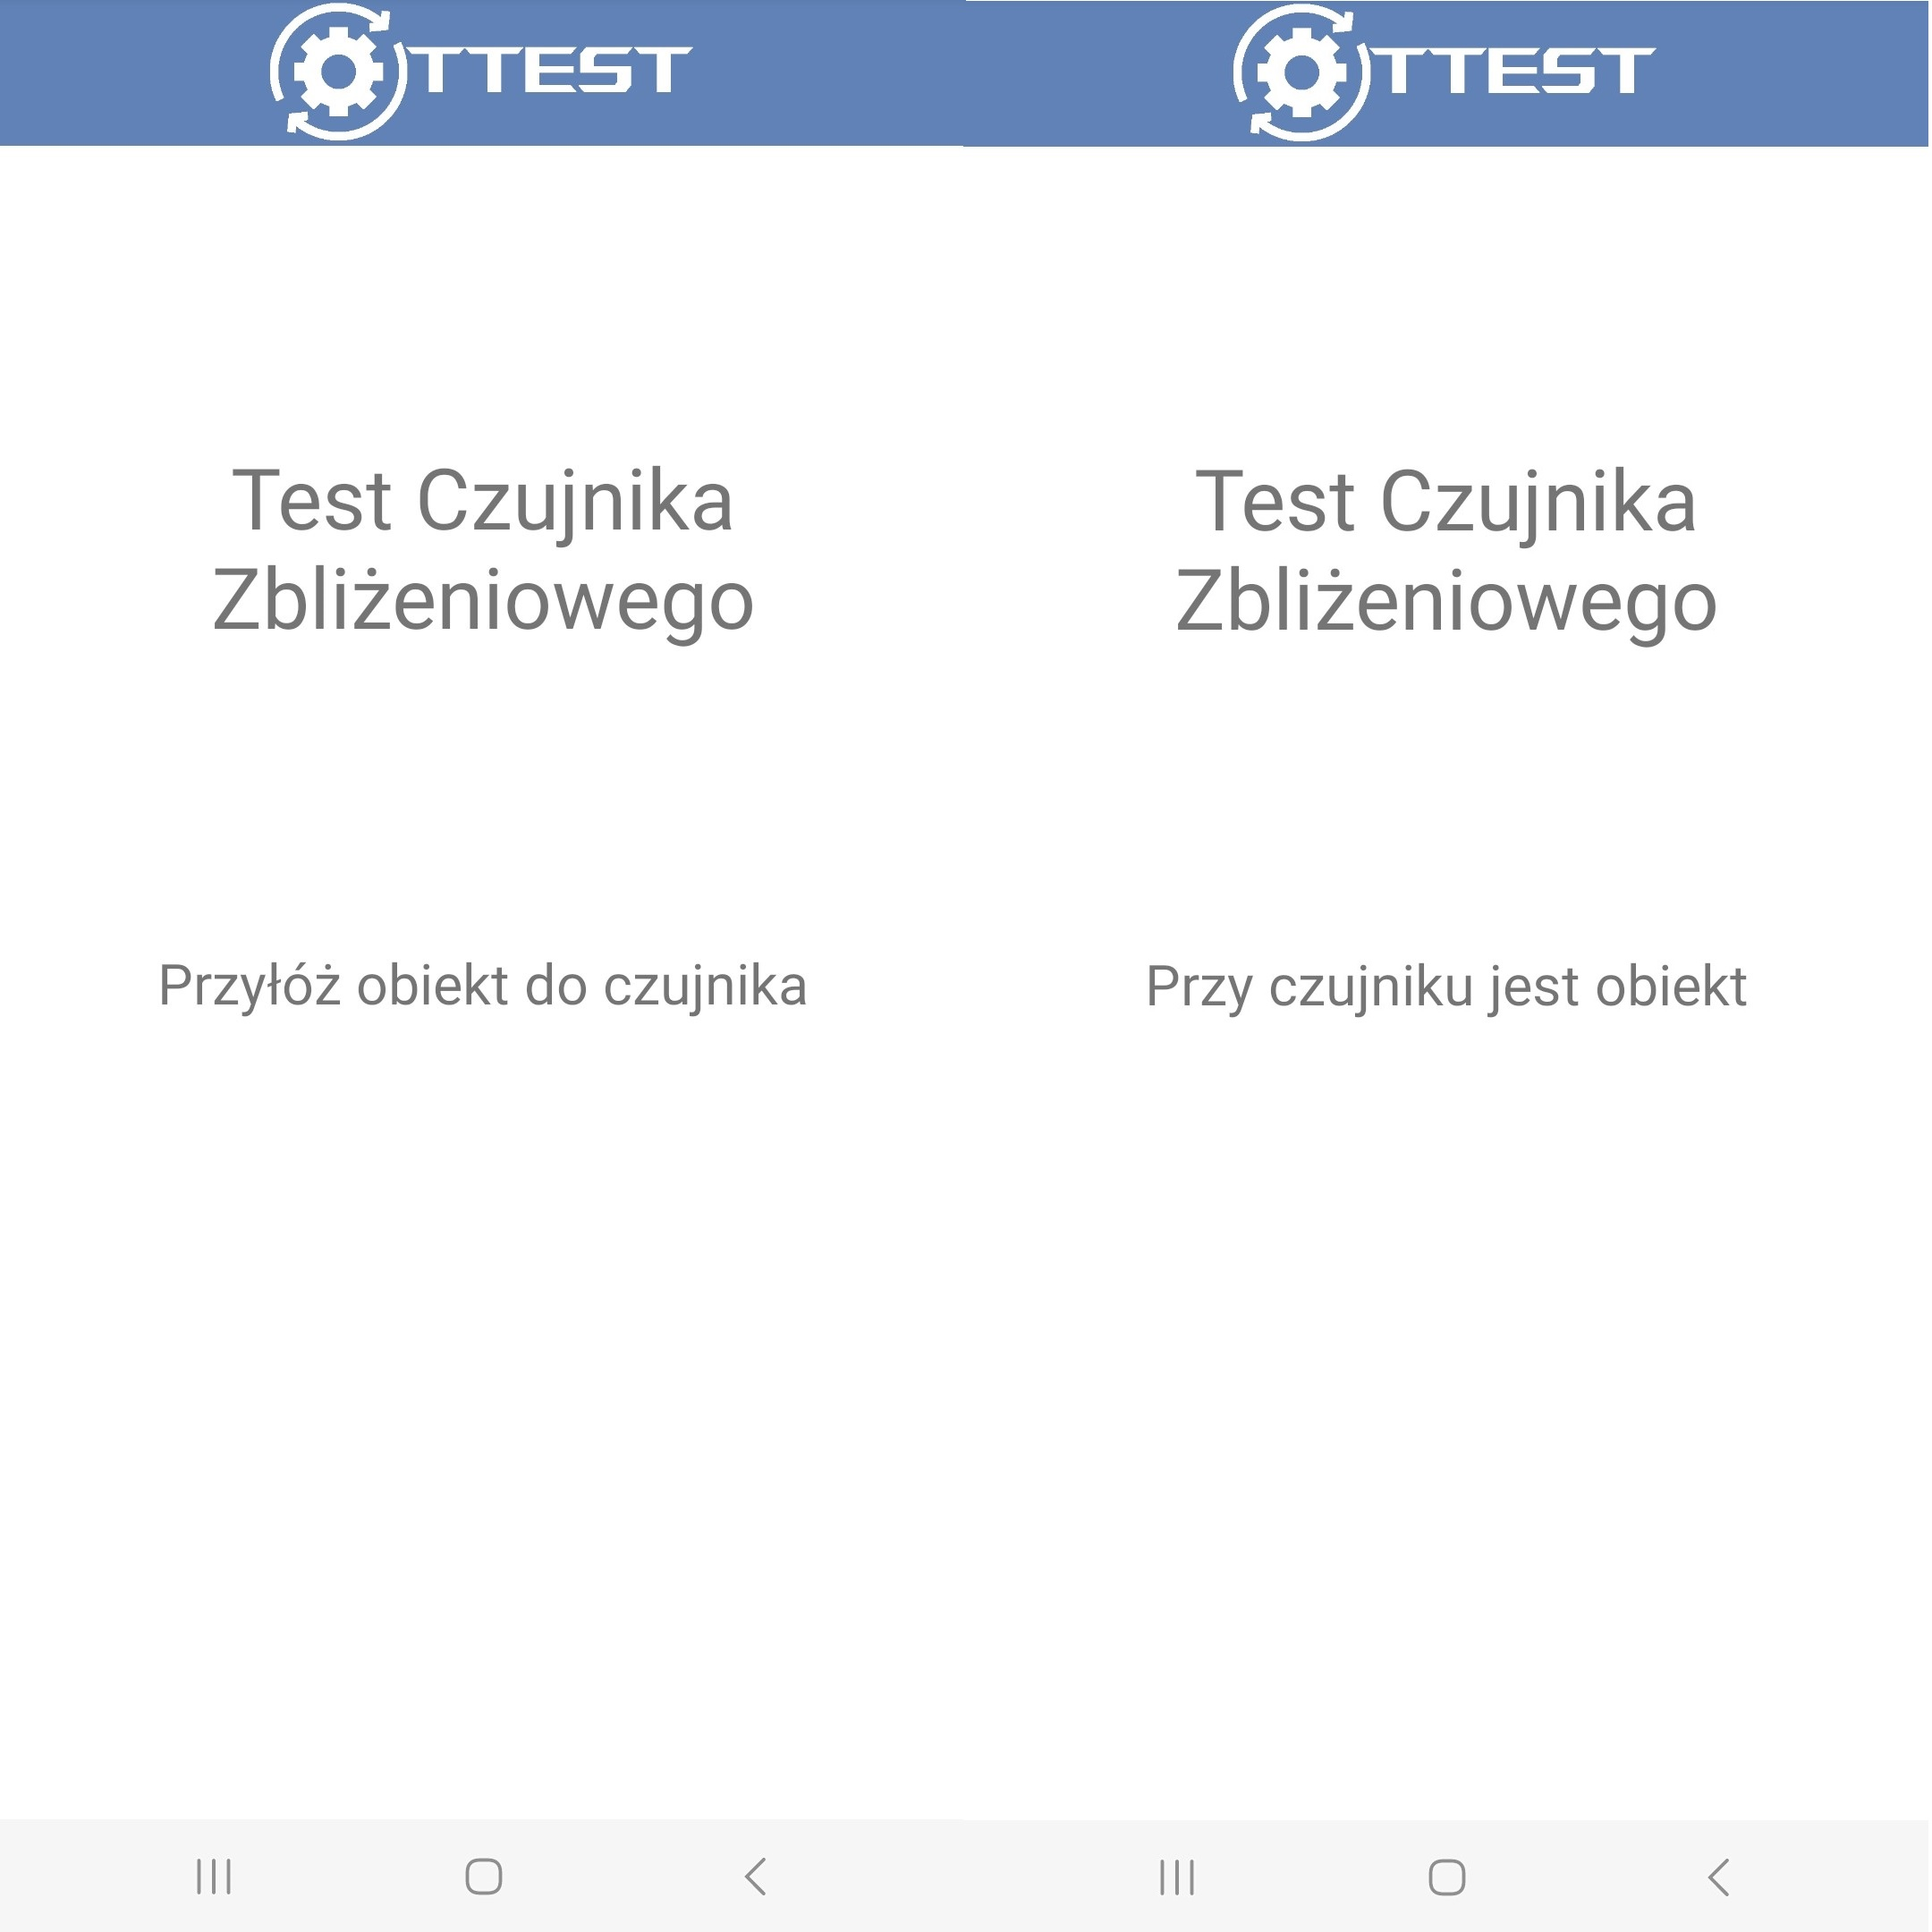
\includegraphics[angle=360, width=0.65\textwidth]{rys/punkt5/zblizeniowy.jpg}
		\caption{Przebieg testowania czujnika zbliżeniowego}
		\label{rys:zblizeniowy}
	\end{center}
\end{figure}   

\newpage


\subsection{Testowanie lokalizacji}

Zadania jakie ma spełniać test lokalizacji zbliżeniiowego przedstawione są w tabeli \ref{tab:tablica_gps}. Jako "X" w kolumnie "Tak" lub "Nie", oznaczamy pomyślny lub niepomyślny przebieg poszczególnych zadań. Całość testu podsumowana jest rzutami ekranu \ref{rys:gps} wykonanymi podczas testowania jako potwierdzenie wykonanego testu.

\begin{tabela}
	{Testowanie lokalizacji}	%opis w spisie tabel
	{Testowanie lokalizacji}	%opis przy tabeli
	{
		\begin{tabular}{|c|c|c|c|c|} \hline
			\textbf{lp} & \textbf{Zadania do przetestowania} & \textbf{Tak} & \textbf{Nie} \\ \hline
			1 & Po naciśnieciu na guzik wyświatla się adres obecnej lokalizacji  & X & ~ \\ \hline
			2 & Po naciśnieciu na guzik wyświatla się komunikat z współrzędnymi & X & ~ \\ \hline
	\end{tabular}	}
	\label{tab:tablica_gps}
\end{tabela}

Obrazek \ref{rys:gps} przedstawia zrzuty ekranu potwierdzające pomyślny przebieg testu.

\begin{figure}[!hbt]
	\begin{center}
		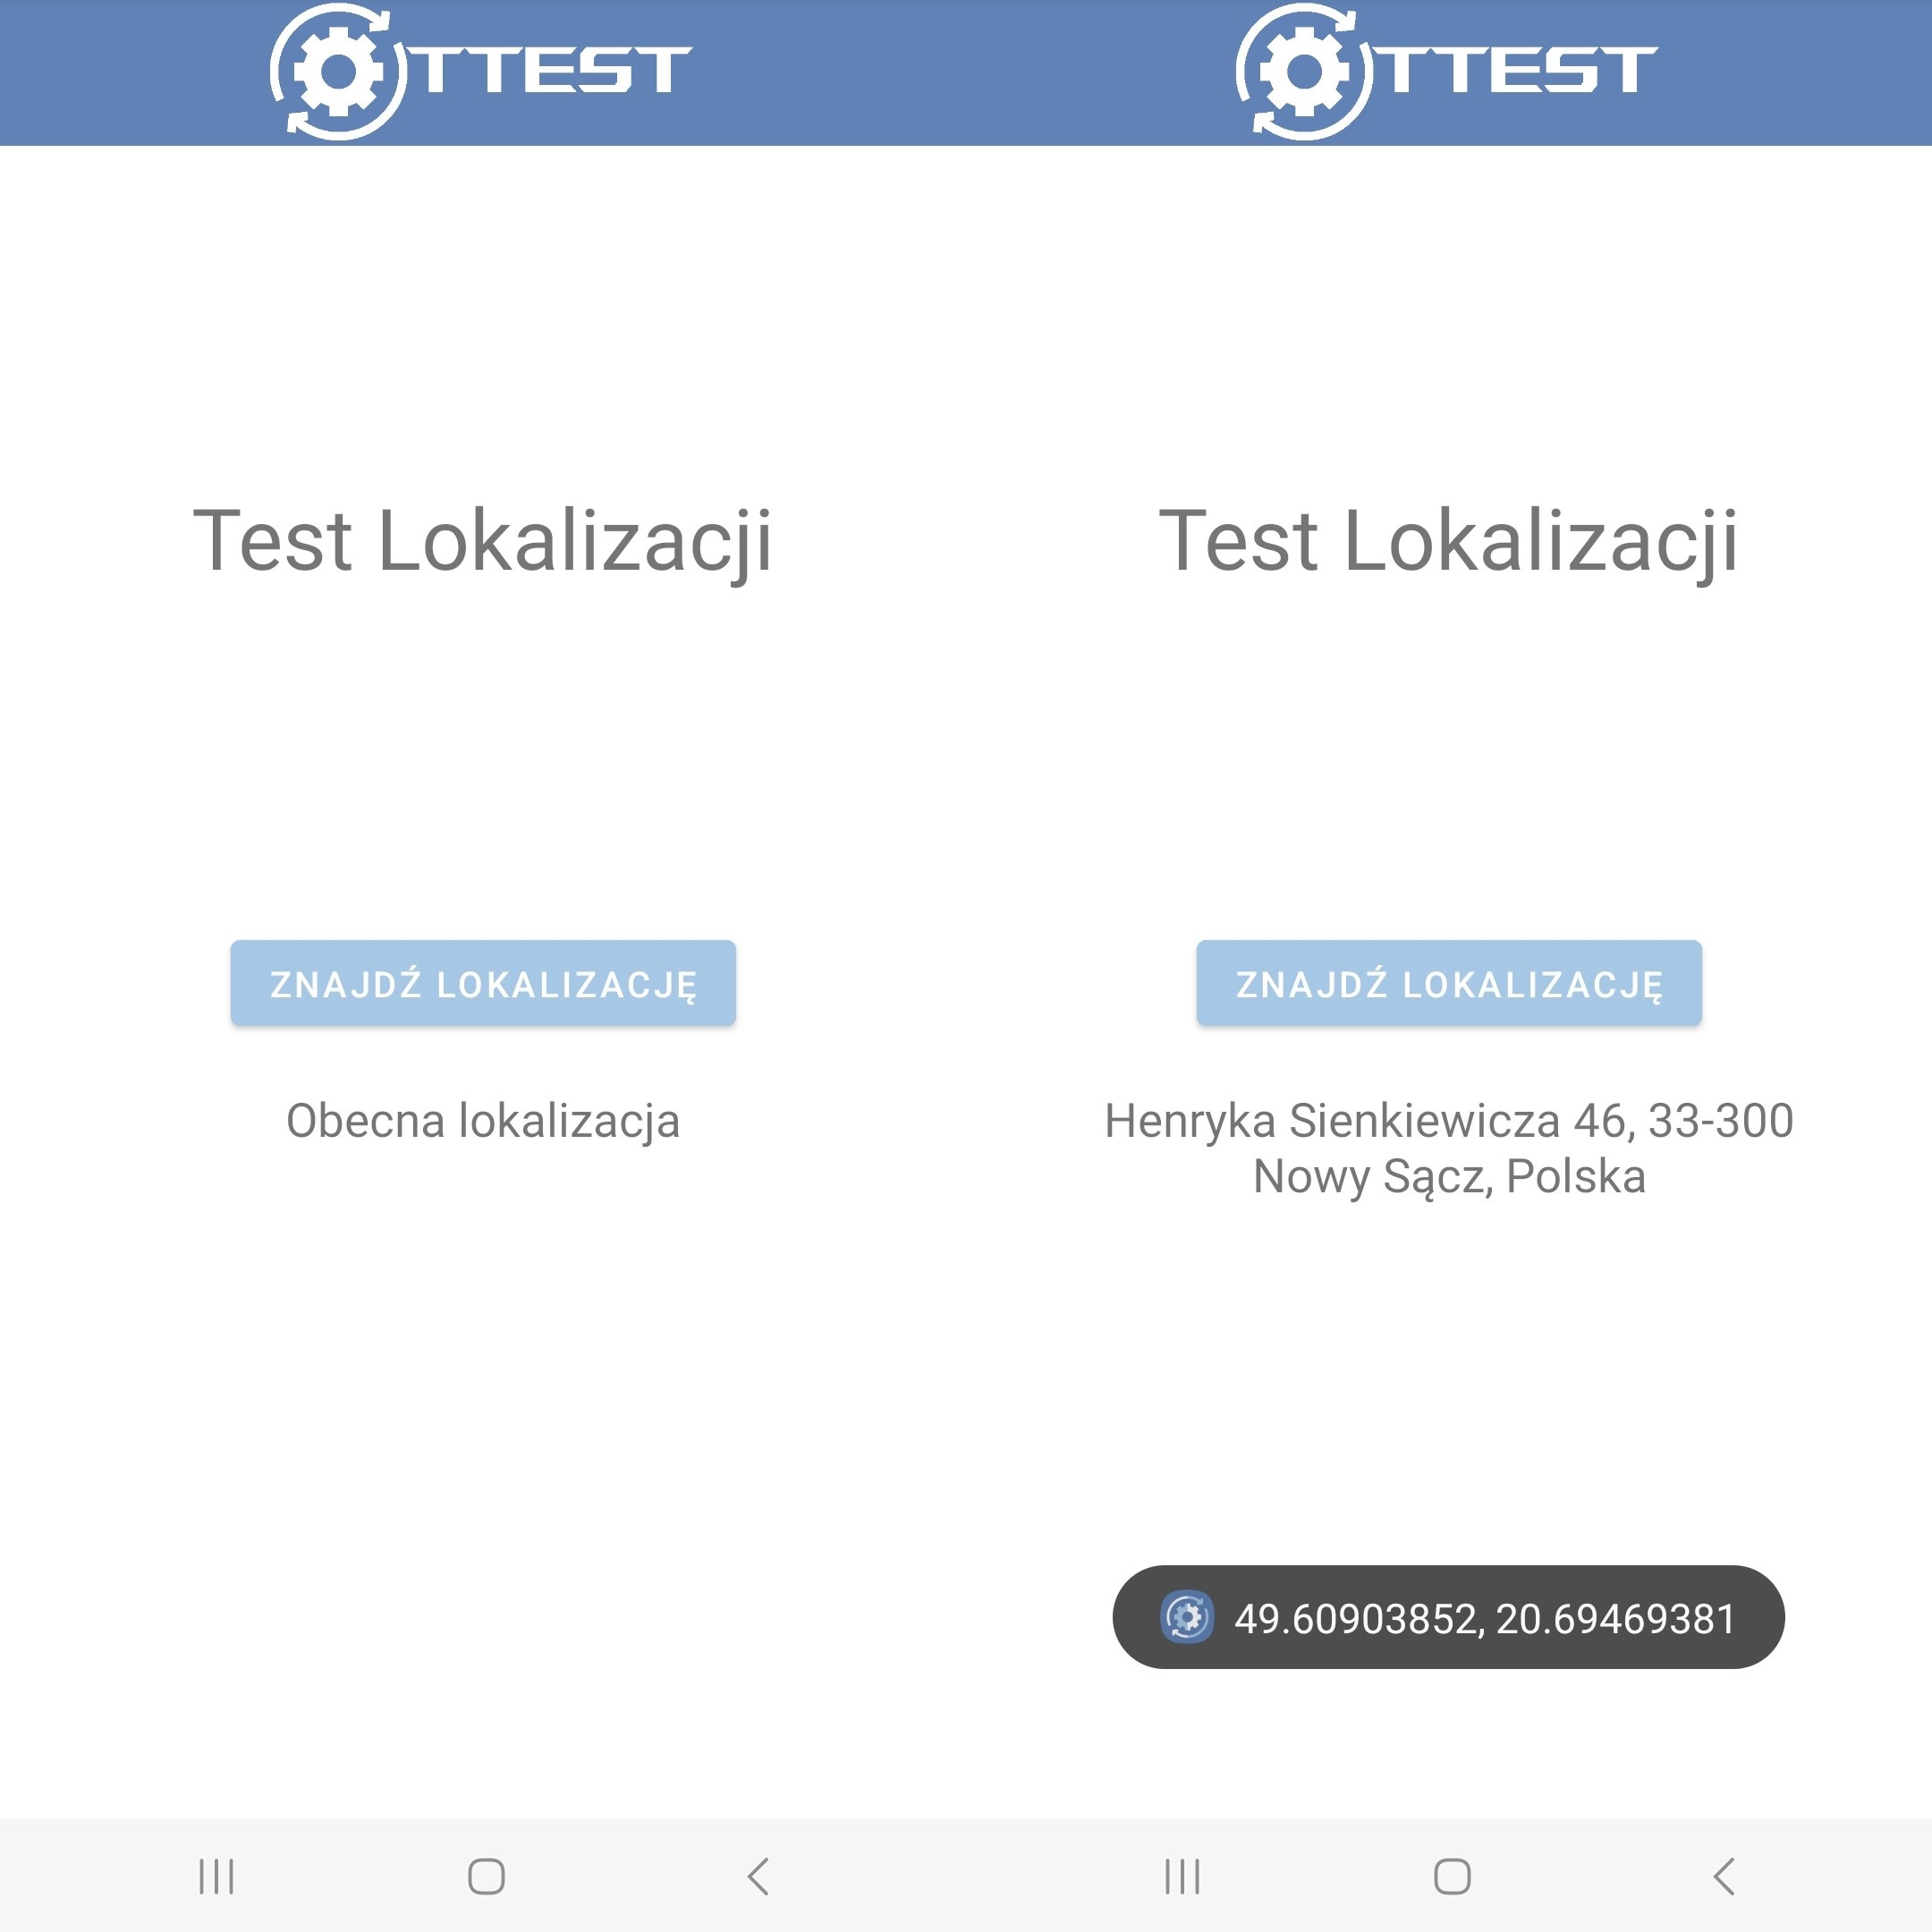
\includegraphics[angle=360, width=0.65\textwidth]{rys/punkt5/gps.jpg}
		\caption{Przebieg testowania lokalizacji}
		\label{rys:gps}
	\end{center}
\end{figure} 

\newpage


\subsection{Testowanie wifi}  

Zadania jakie ma spełniać test wifi przedstawione są w tabeli \ref{tab:tablica_wifi}. Jako "X" \\ w kolumnie "Tak" lub "Nie", oznaczamy pomyślny lub niepomyślny przebieg poszczególnych zadań. Całość testu podsumowana jest rzutami ekranu \ref{rys:wifi} wykonanymi podczas testowania jako potwierdzenie wykonanego testu.

\begin{tabela}
	{Testowanie wifi}	%opis w spisie tabel
	{Testowanie wifi}	%opis przy tabeli
	{
		\begin{tabular}{|c|c|c|c|c|} \hline
			\textbf{lp} & \textbf{Zadania do przetestowania} & \textbf{Tak} & \textbf{Nie} \\ \hline
			1 & Pojawia się informacja o statusie wifi & X & ~ \\ \hline
			2 & Po naciśnieciu na guzik pojawia się adres IP telefonu & X & ~ \\ \hline
			3 & Po naciśnieciu na guzik pojawia się adres MAC routera & X & ~ \\ \hline
			4 & Po naciśnieciu na guzik pojawia się SSID sieci & X & ~ \\ \hline
			5 & Po naciśnieciu na guzik pojawia się wzkaźnik mocy & X & ~ \\ \hline
	\end{tabular}	}
	\label{tab:tablica_wifi}
\end{tabela}

Obrazek \ref{rys:wifi} przedstawia zrzuty ekranu potwierdzające pomyślny przebieg testu.

\begin{figure}[!hbt]
	\begin{center}
		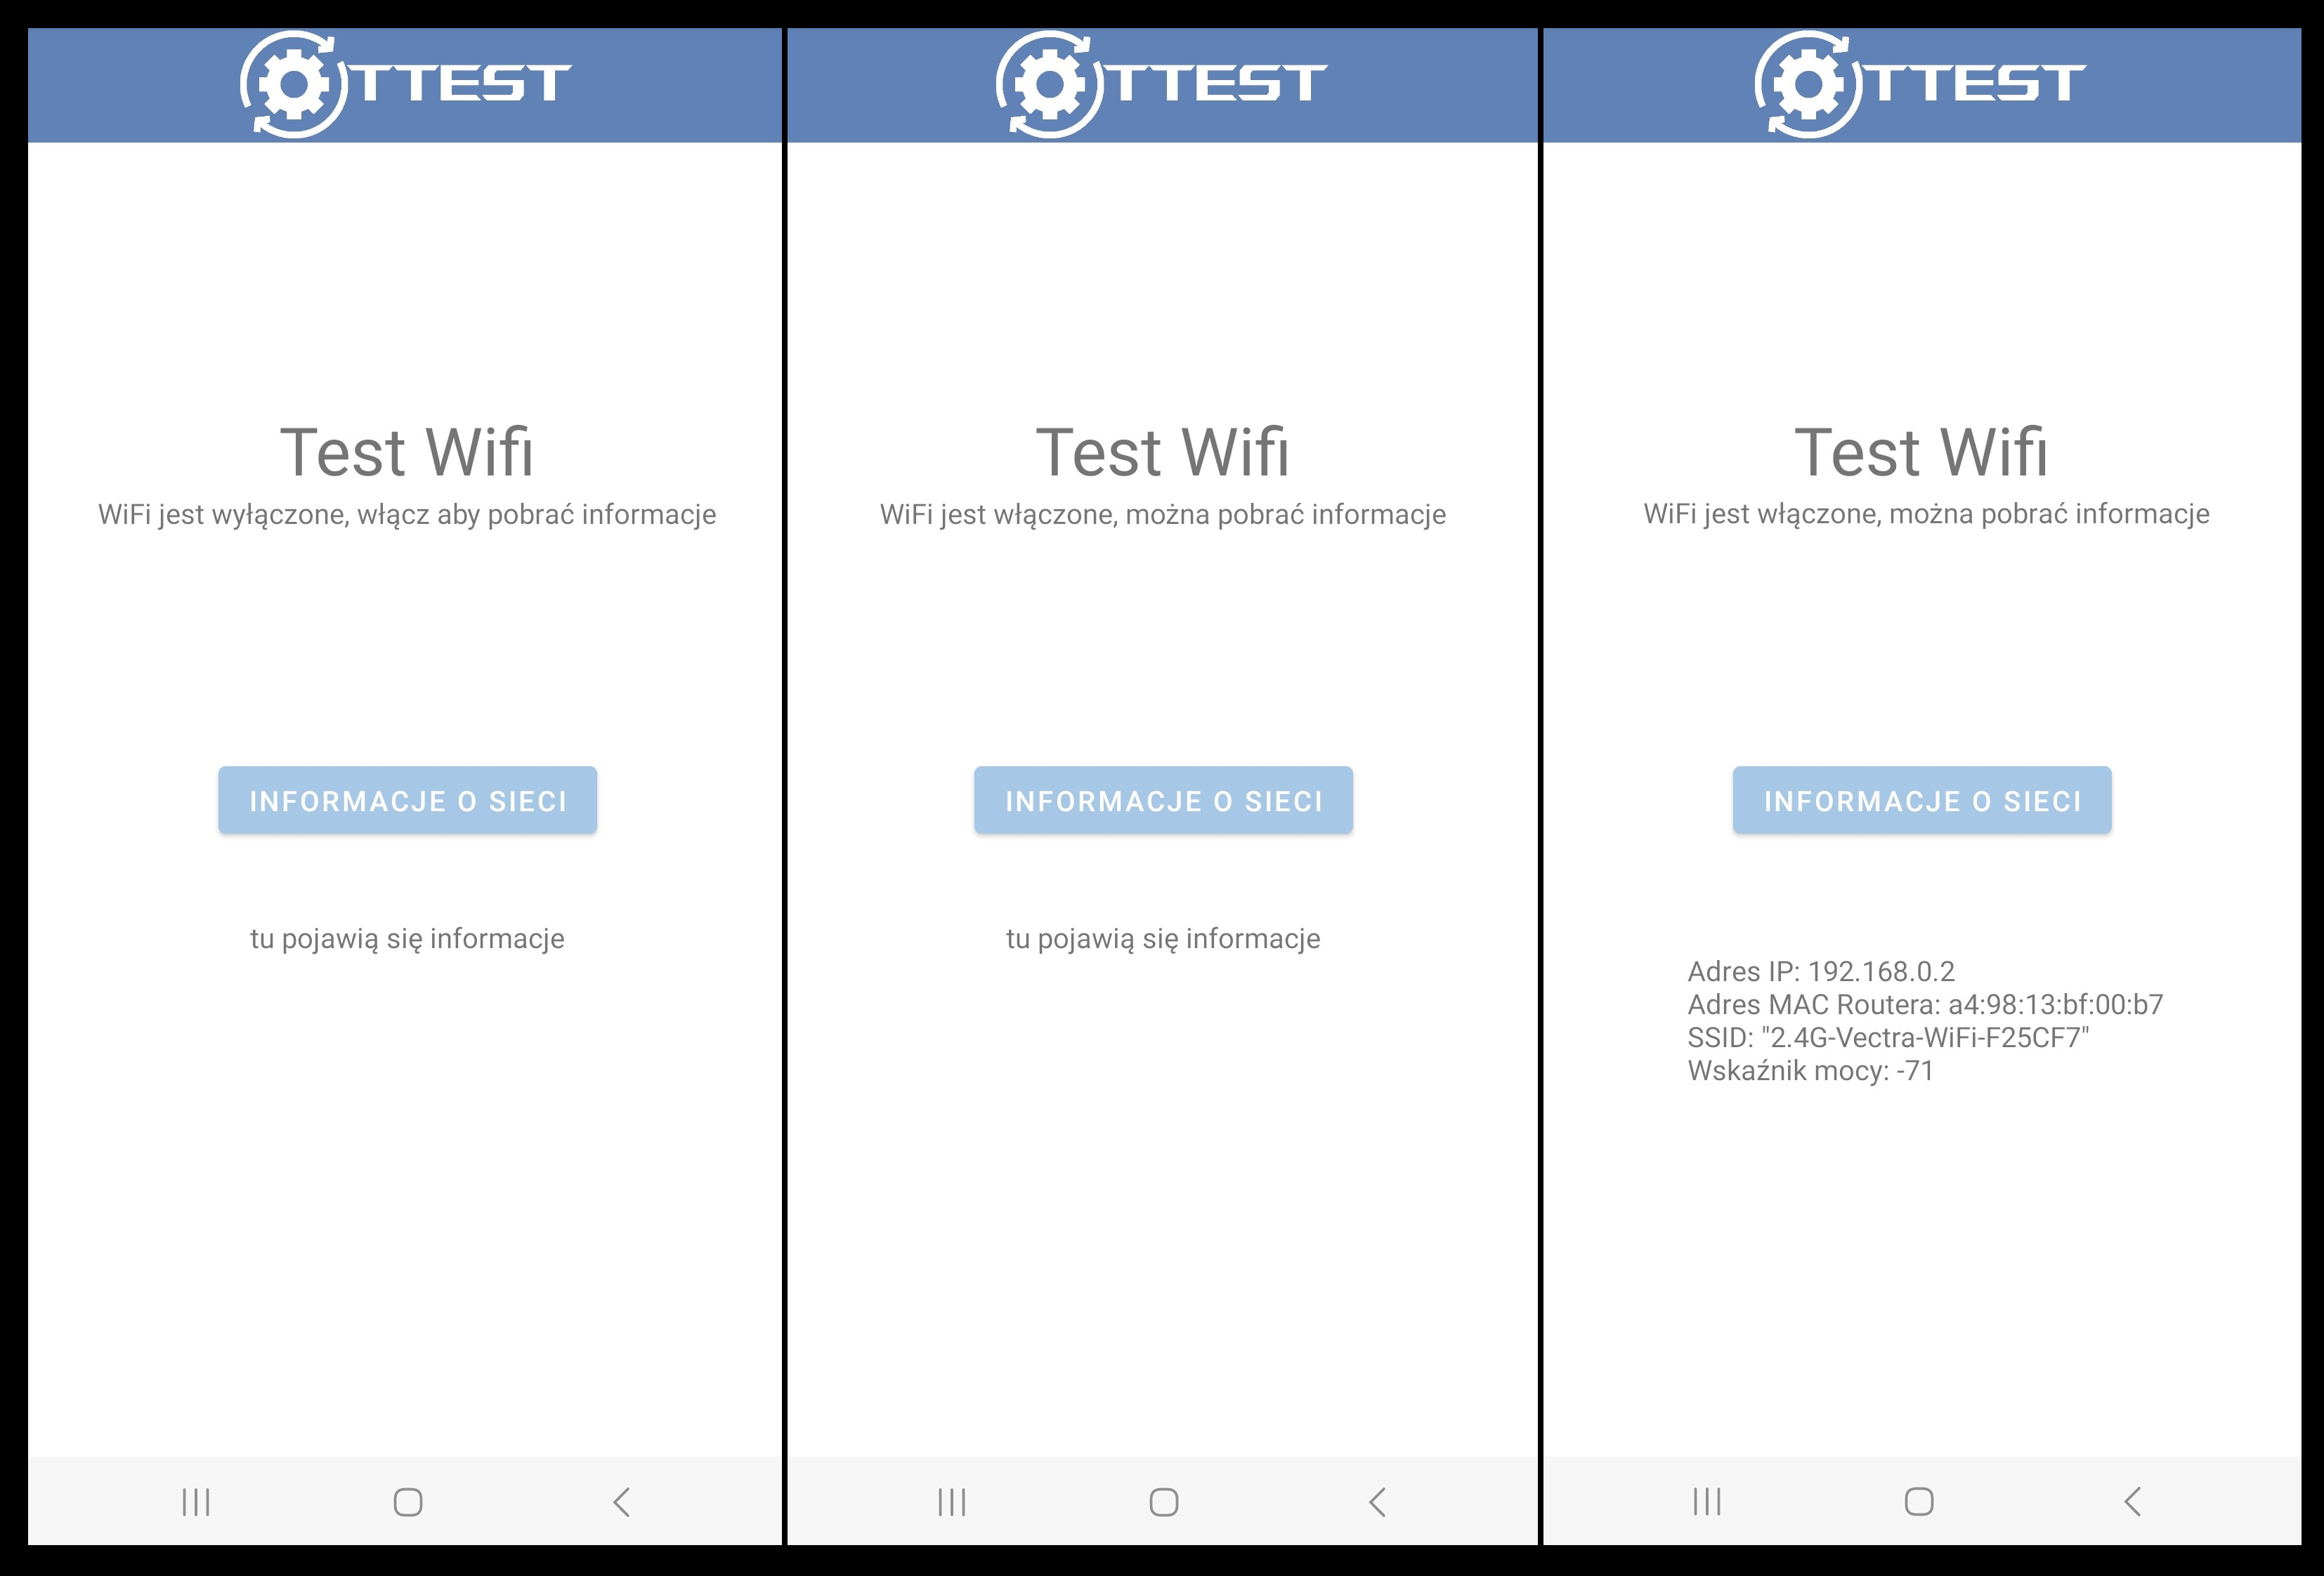
\includegraphics[angle=360, width=0.90\textwidth]{rys/punkt5/wifi.png}
		\caption{Przebieg testowania wifi}
		\label{rys:wifi}
	\end{center}
\end{figure} 

\newpage


\subsection{Testowanie dźwięku}

Zadania jakie ma spełniać test dźwięku przedstawione są w tabeli \ref{tab:tablica_dzwiek}. Jako "X" \\ w kolumnie "Tak" lub "Nie", oznaczamy pomyślny lub niepomyślny przebieg poszczególnych zadań. Całość testu podsumowana jest rzutami ekranu \ref{rys:dzwiek} wykonanymi podczas testowania jako potwierdzenie wykonanego testu.

\begin{tabela}
	{Testowanie dźwięku}	%opis w spisie tabel
	{Testowanie dźwięku}	%opis przy tabeli
	{
		\begin{tabular}{|c|c|c|c|c|} \hline
			\textbf{lp} & \textbf{Zadania do przetestowania} & \textbf{Tak} & \textbf{Nie} \\ \hline
			1 & Po naciśnięciu na guzik z głośników słychać śpiew ptaków & X & ~ \\ \hline
			2 & Wyświetlenie komunikatu o rozpoczęciu odtwarzania nagrania & X & ~ \\ \hline
	\end{tabular}	}
	\label{tab:tablica_dzwiek}
\end{tabela}

Obrazek \ref{rys:dzwiek} przedstawia zrzuty ekranu potwierdzające pomyślny przebieg testu.

\begin{figure}[!hbt]
	\begin{center}
		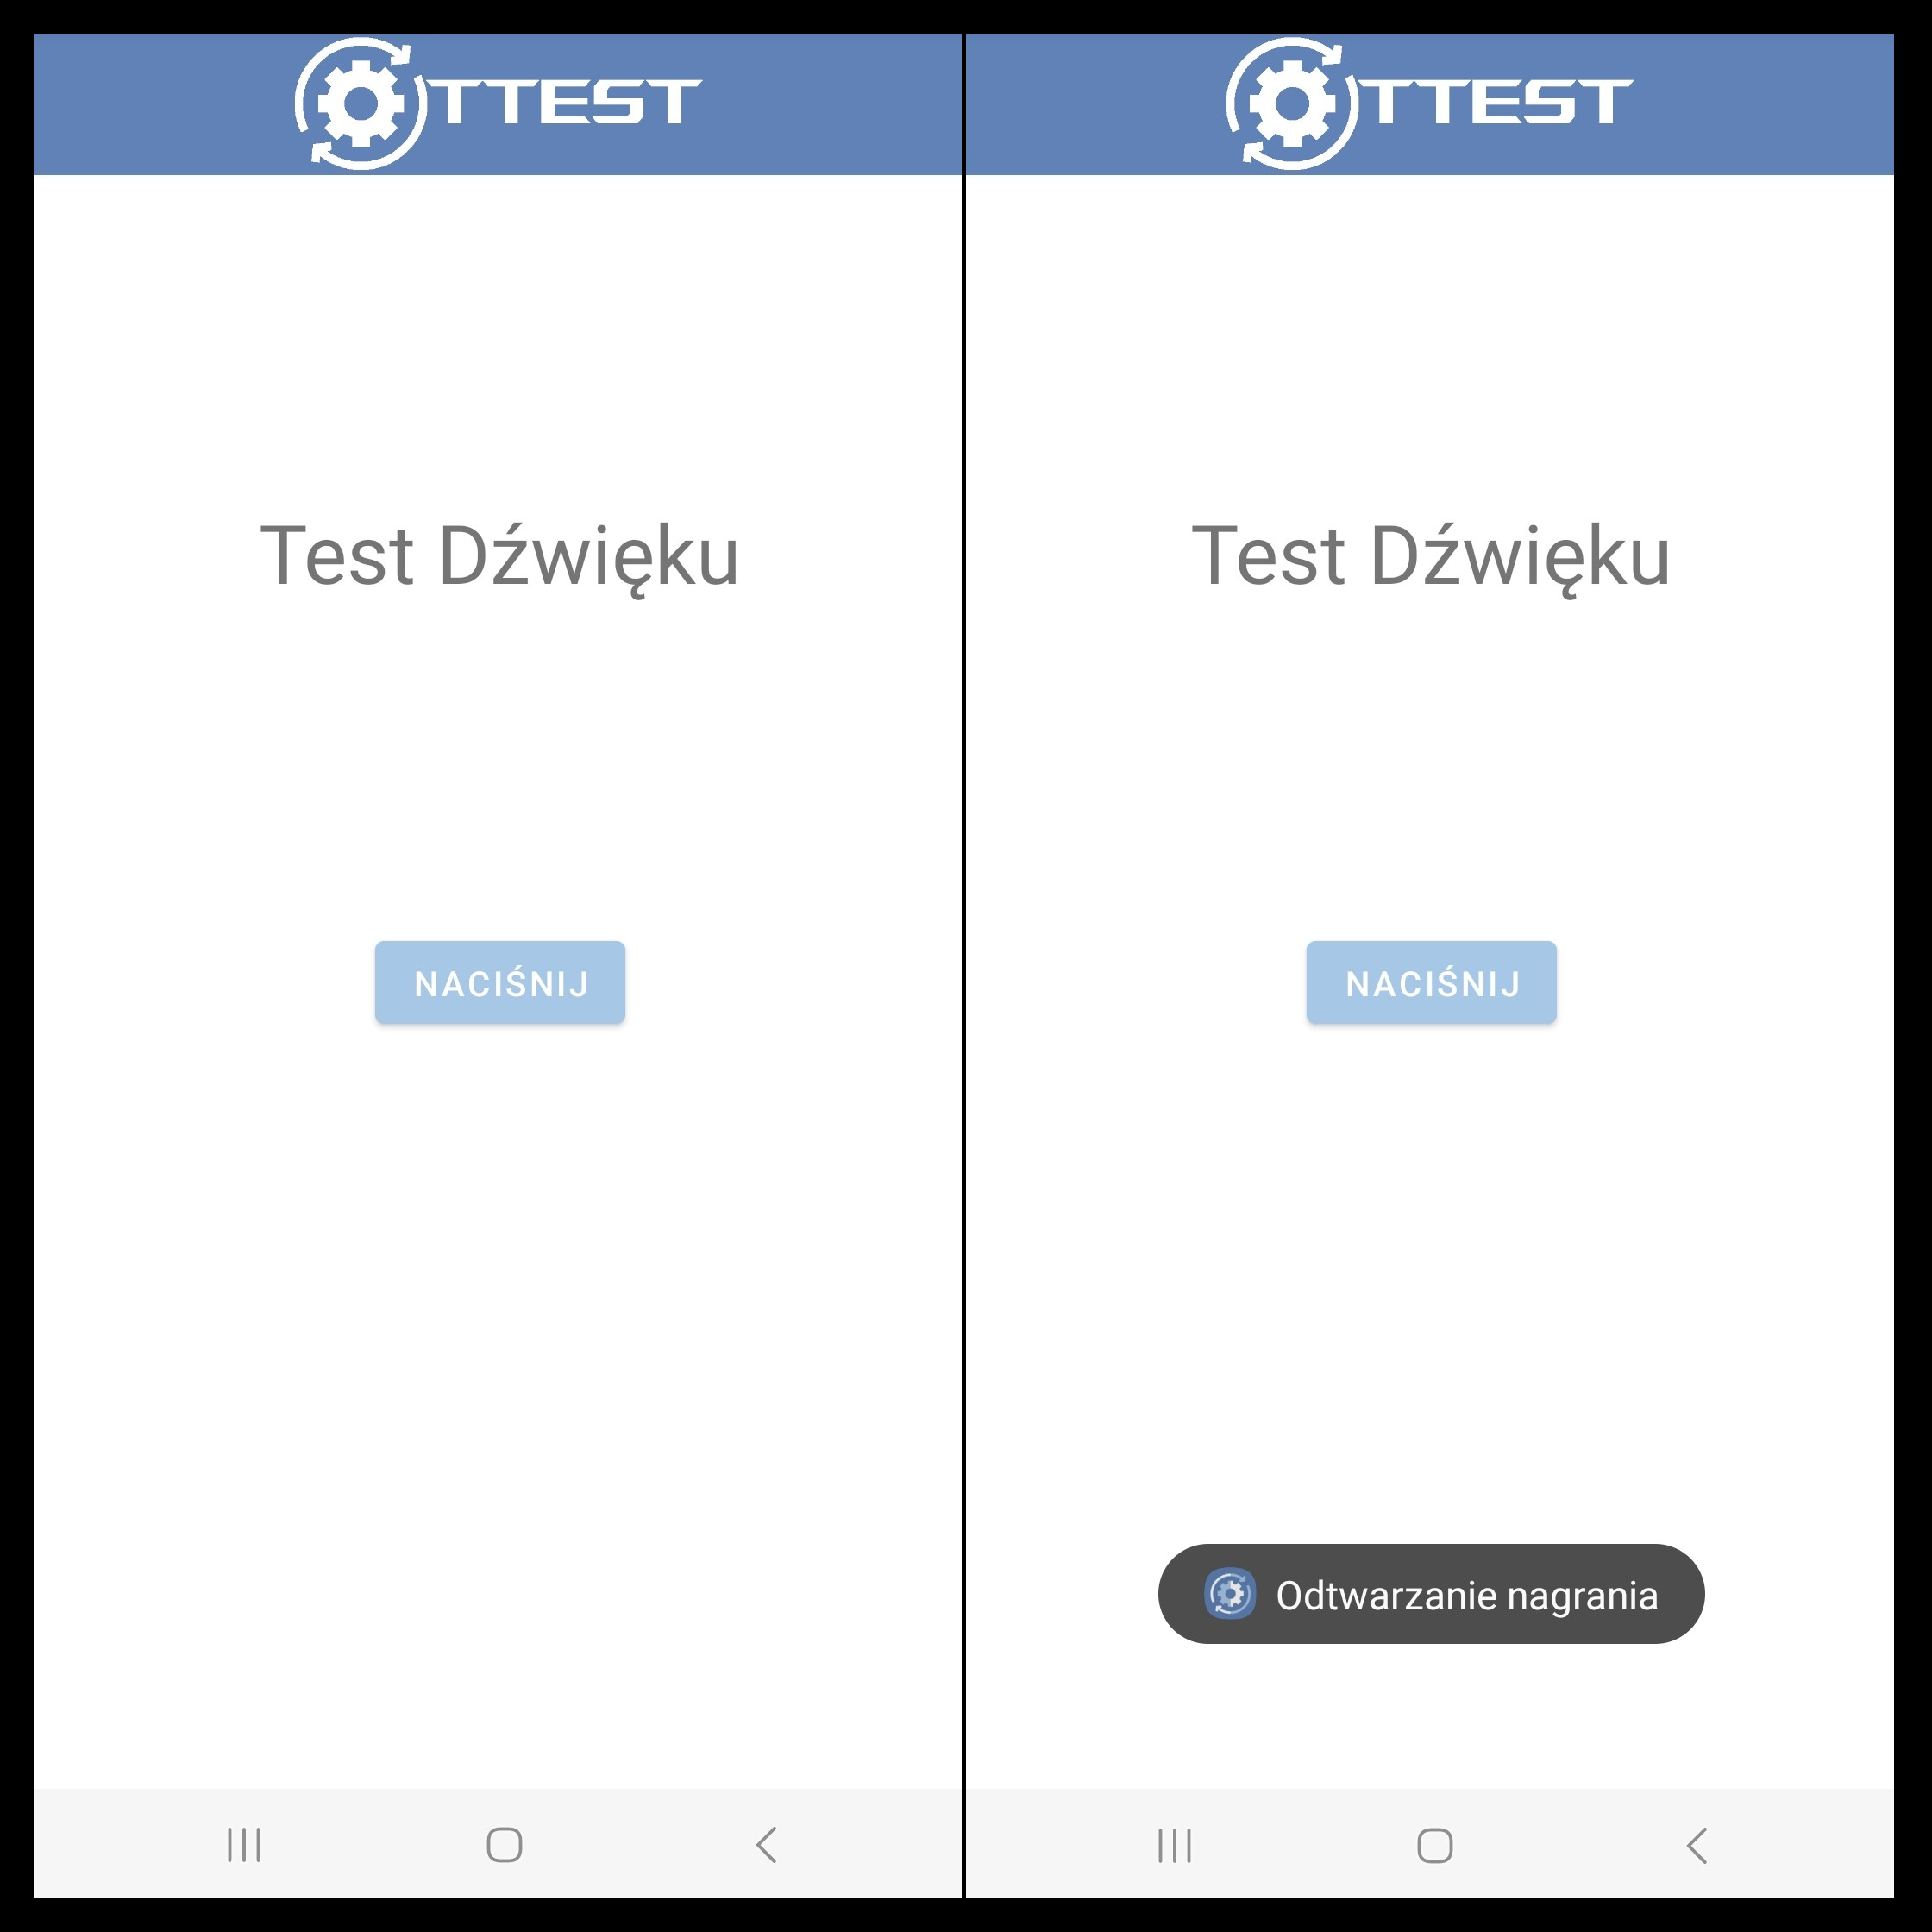
\includegraphics[angle=360, width=0.65\textwidth]{rys/punkt5/dzwiek.png}
		\caption{Przebieg testowania dźwięku}
		\label{rys:dzwiek}
	\end{center}
\end{figure} 

\newpage


\subsection{Testowanie mikrofonu}

Zadania jakie ma spełniać test mikrofonu przedstawione są w tabeli \ref{tab:tablica_mikrofon}. Jako "X" \\ w kolumnie "Tak" lub "Nie", oznaczamy pomyślny lub niepomyślny przebieg poszczególnych zadań. Całość testu podsumowana jest rzutami ekranu \ref{rys:mikrofon} wykonanymi podczas testowania jako potwierdzenie wykonanego testu.

\begin{tabela}
	{Testowanie mikrofonu}	%opis w spisie tabel
	{Testowanie mikrofonu}	%opis przy tabeli
	{
		\begin{tabular}{|c|c|c|c|c|} \hline
			\textbf{lp} & \textbf{Zadania do przetestowania} & \textbf{Tak} & \textbf{Nie} \\ \hline
			1 & Naciśnięcie na guzik "START" zaczyna nagrywanie & X & ~ \\ \hline
			2 & Po naciśnięciu na guzik "START" wyświetla się adekwatny komunikat & X & ~ \\ \hline
			3 & Naciśnięcie na guzik "STOP" kończy nagrywanie & X & ~ \\ \hline
			4 & Po naciśnięciu na guzik "STOP" wyświetla się adekwatny komunikat & X & ~ \\ \hline
			5 & Naciśnięcie na guzik "PLAY" oddtwarza nagranie & X & ~ \\ \hline
			6 &  Po naciśnięciu na guzik "PLAY" wyświetla się adekwatny komunikat & X & ~ \\ \hline
	\end{tabular}	}
	\label{tab:tablica_mikrofon}
\end{tabela}

Obrazek \ref{rys:mikrofon} przedstawia zrzuty ekranu potwierdzające pomyślny przebieg testu.

\begin{figure}[!hbt]
	\begin{center}
		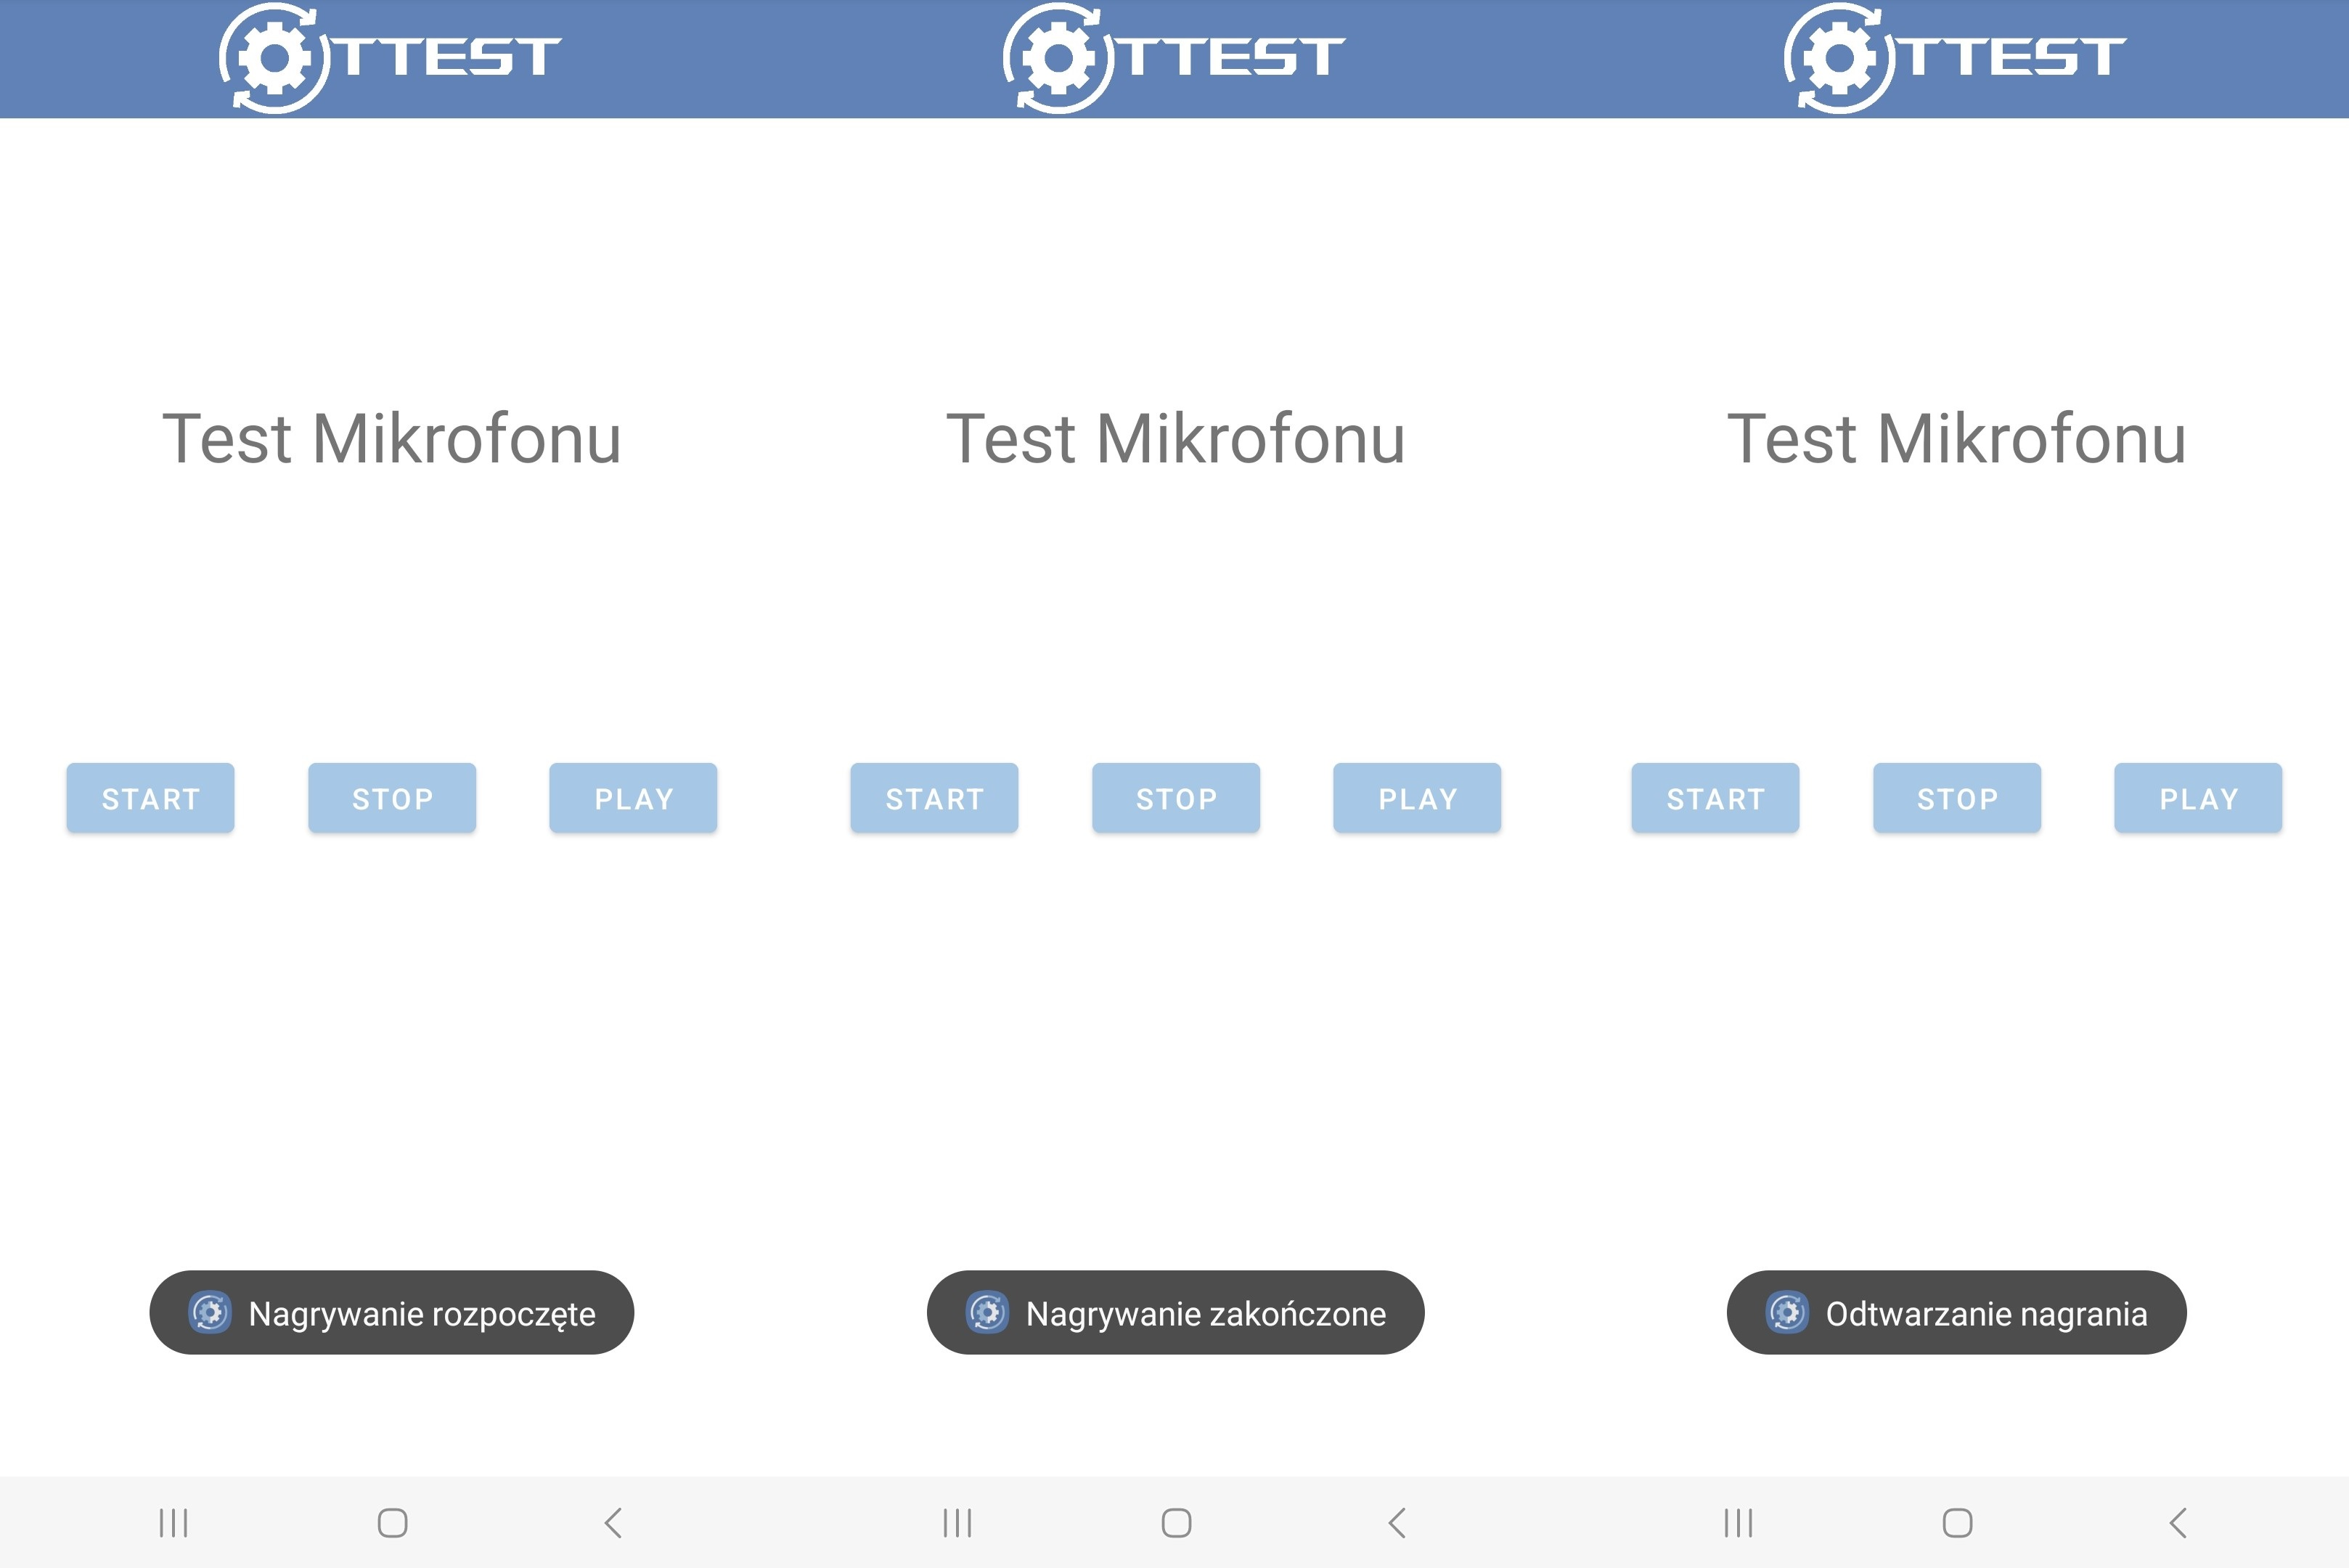
\includegraphics[angle=360, width=0.90\textwidth]{rys/punkt5/mikrofon.jpg}
		\caption{Przebieg testowania mikrofonu}
		\label{rys:mikrofon}
	\end{center}
\end{figure} 

\newpage


\subsection{Testowanie aparatu}

Zadania jakie ma spełniać test mikrofonu przedstawione są w tabeli \ref{tab:tablica_aparat}. Jako "X" \\ w kolumnie "Tak" lub "Nie", oznaczamy pomyślny lub niepomyślny przebieg poszczególnych zadań. Całość testu podsumowana jest rzutami ekranu \ref{rys:aparat} wykonanymi podczas testowania jako potwierdzenie wykonanego testu.

\begin{tabela}
	{Testowanie aparatu}	%opis w spisie tabel
	{Testowanie aparatu}	%opis przy tabeli
	{
		\begin{tabular}{|c|c|c|c|c|} \hline
			\textbf{lp} & \textbf{Zadania do przetestowania} & \textbf{Tak} & \textbf{Nie} \\ \hline
			1 & Po naciśnięciu na guzik "zrób zdjęcie" włącza się aplikacja aparatu & X & ~ \\ \hline
			2 & Można wykonać zdjęcię poprzez naciśnięcie białego guzika & X & ~ \\ \hline
			3 & Jako potwierdzenie wykonania zdjęcia, wyświetla się ono & X & ~ \\ \hline
	\end{tabular}	}
	\label{tab:tablica_aparat}
\end{tabela}

Obrazek \ref{rys:aparat} przedstawia zrzuty ekranu potwierdzające pomyślny przebieg testu.

\begin{figure}[!hbt]
	\begin{center}
		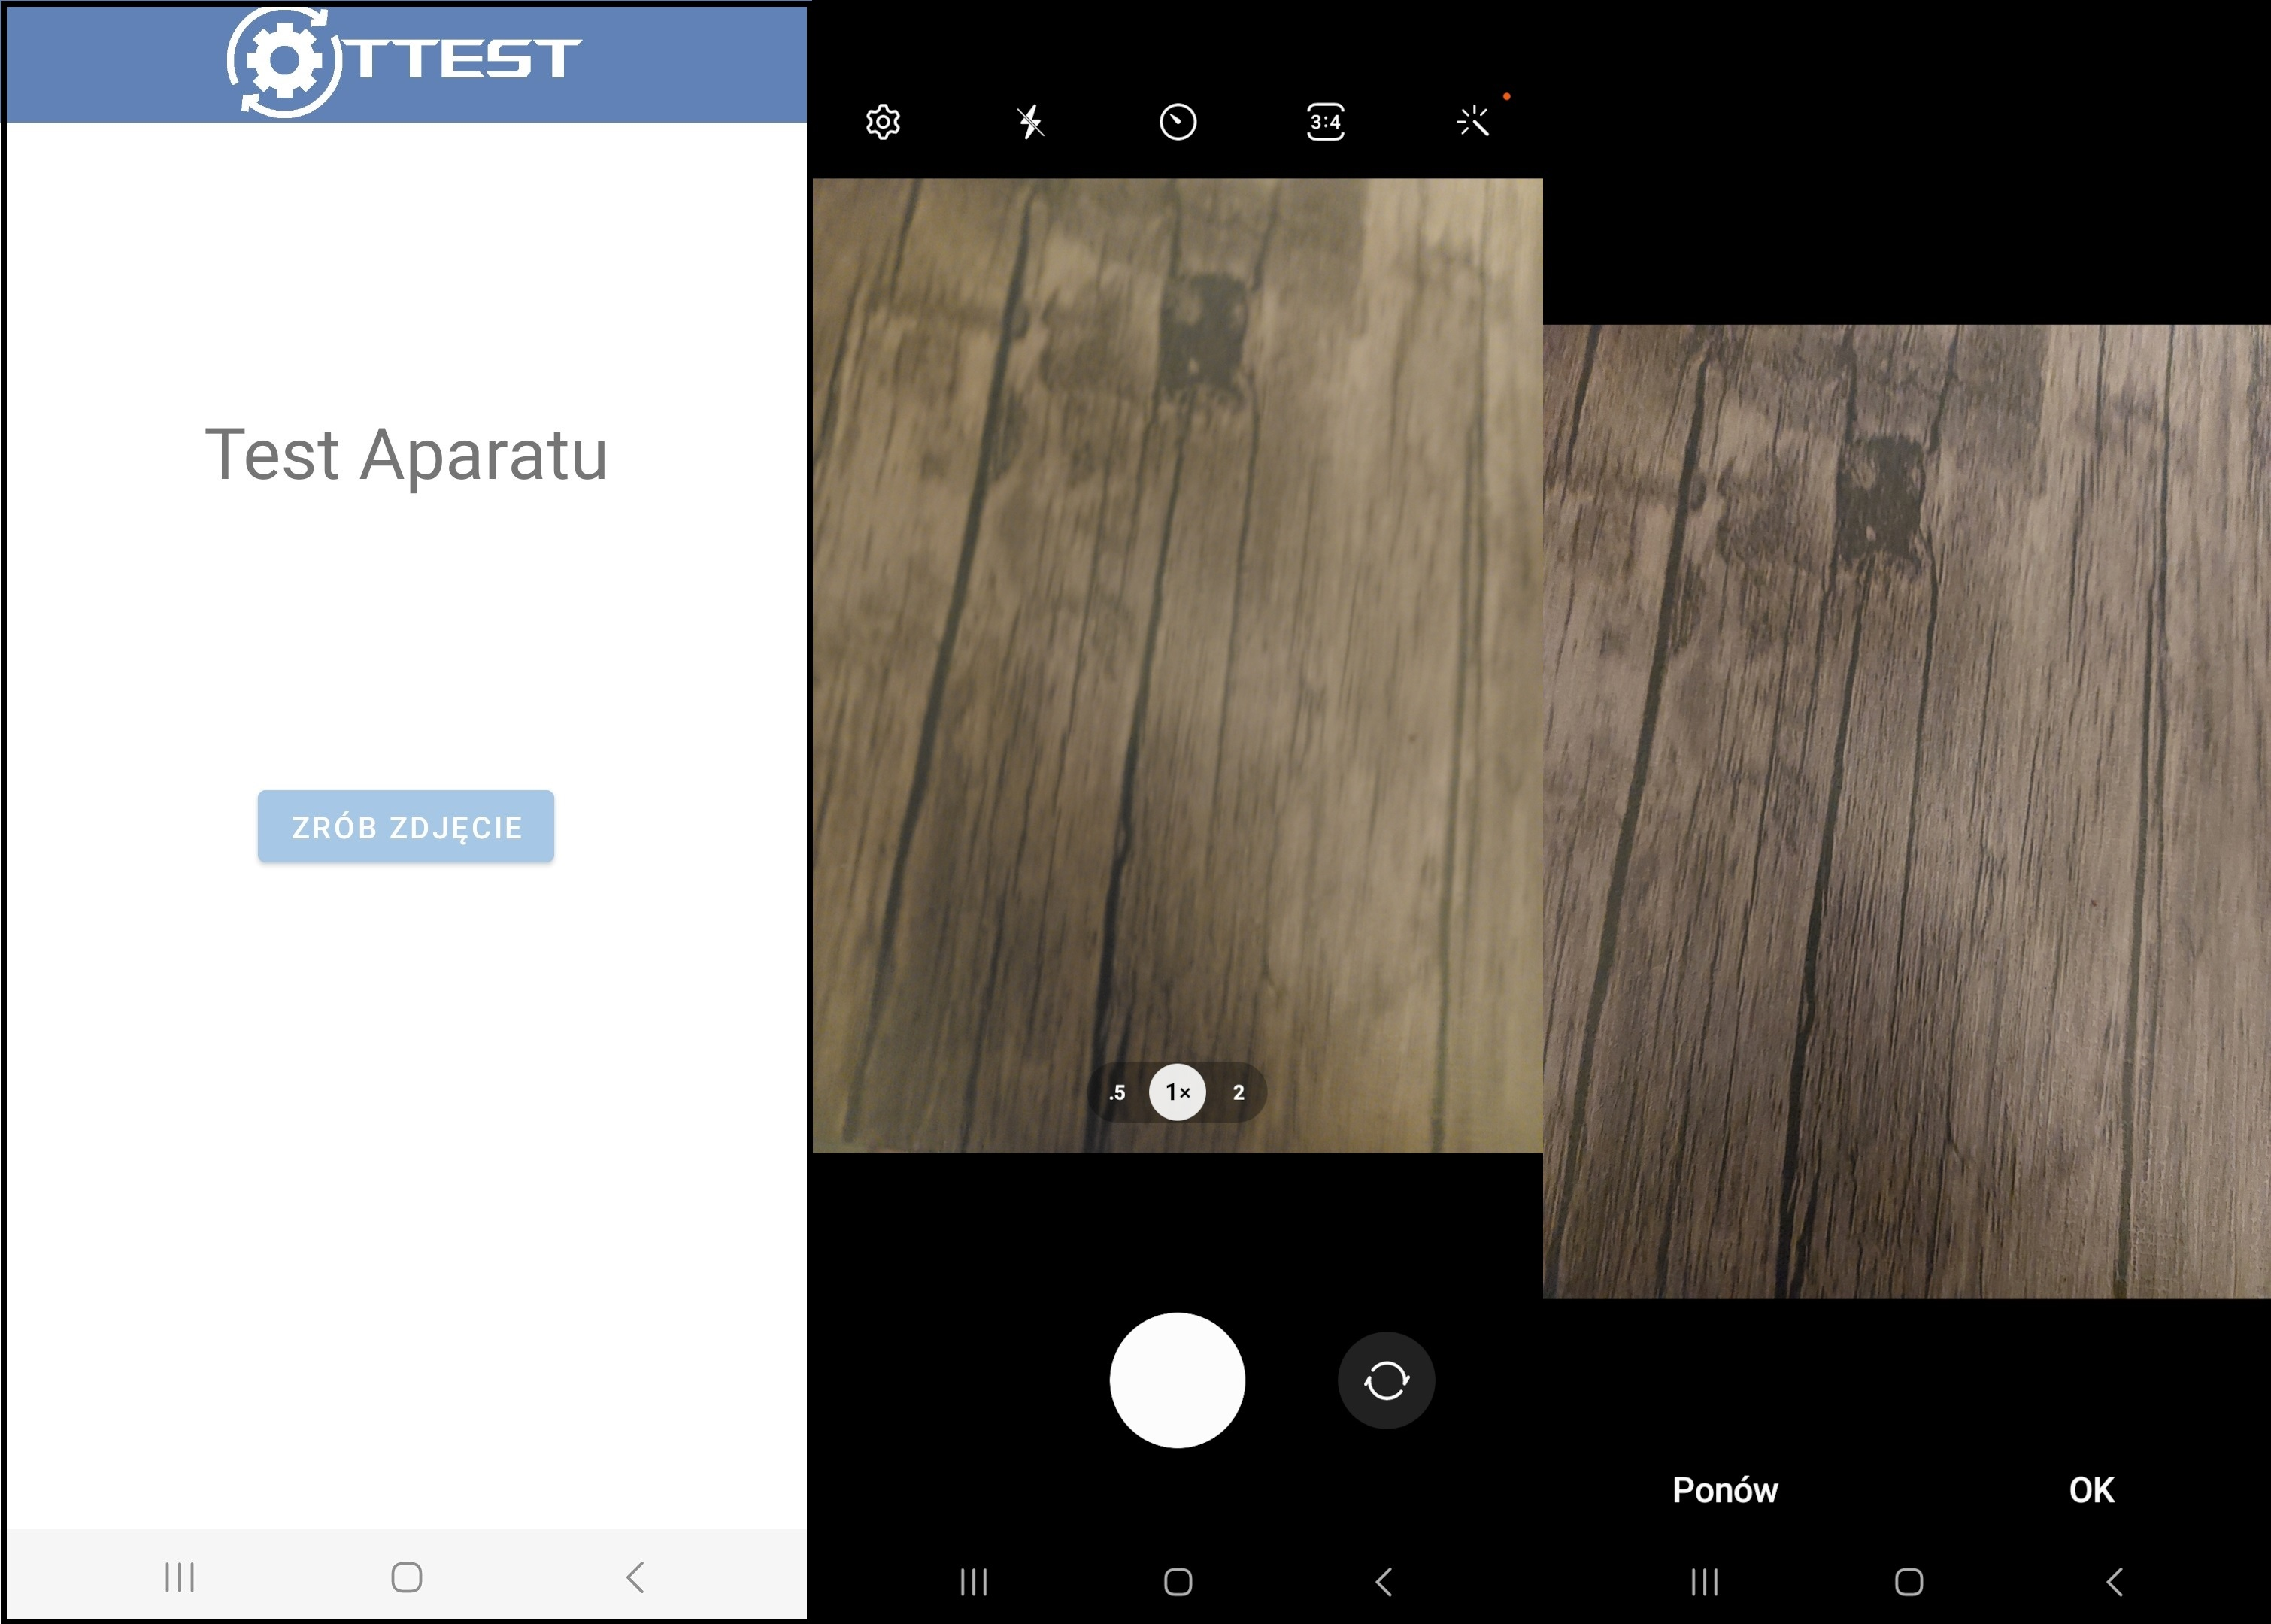
\includegraphics[angle=360, width=0.90\textwidth]{rys/punkt5/aparat.jpg}
		\caption{Przebieg testowania aparatu}
		\label{rys:aparat}
	\end{center}
\end{figure} 

\newpage


\subsection{Testowanie menu}

Zadania jakie ma spełniać menu przedstawione są w tabeli \ref{tab:tablica_menu}. Jako "X" w kolumnie "Tak" lub "Nie", oznaczamy pomyślny lub niepomyślny przebieg poszczególnych zadań. Całość testu podsumowana jest rzutami ekranu \ref{rys:menu} wykonanymi podczas testowania jako potwierdzenie wykonanego testu.

\begin{tabela}
	{Testowanie menu}	%opis w spisie tabel
	{Testowanie menu}	%opis przy tabeli
	{
		\begin{tabular}{|c|c|c|c|} \hline
			\textbf{lp} & \textbf{Zadania do przetestowania} & \textbf{Tak} & \textbf{Nie} \\ \hline
			1 & Guzik "Latarka" przekierwuje do testu latarki & X & ~ \\ \hline
			2 & Guzik "Tryb ciemny" przekierwuje do testu trybu ciemnego & X & ~ \\ \hline
			3 & Guzik "Zbliżeniowy" przekierwuje do testu czujnika zbliżeniowego & X & ~ \\ \hline
			4 & Guzik "GPS" przekierwuje do testu lokalizacji & X & ~ \\ \hline
			5 & Guzik "Wifi" przekierwuje do testu wifi & X & ~ \\ \hline
			6 & Guzik "Dźwięk" przekierwuje do testu dźwięku & X & ~ \\ \hline
			7 & Guzik "Mikrofon" przekierwuje do testu mikrofonu & X & ~ \\ \hline
			8 & Guzik "Aparat" przekierwuje do testu aparatu & X & ~ \\ \hline
			9 & Guzik "Wyniki" przekierwuje do podsumowania testów & X & ~ \\ \hline
	\end{tabular}	}
	\label{tab:tablica_menu}
\end{tabela}

Obrazek \ref{rys:menu} przedstawia zrzuty ekranu potwierdzające pomyślny przebieg testu.

\begin{figure}[!hbt]
	\begin{center}
		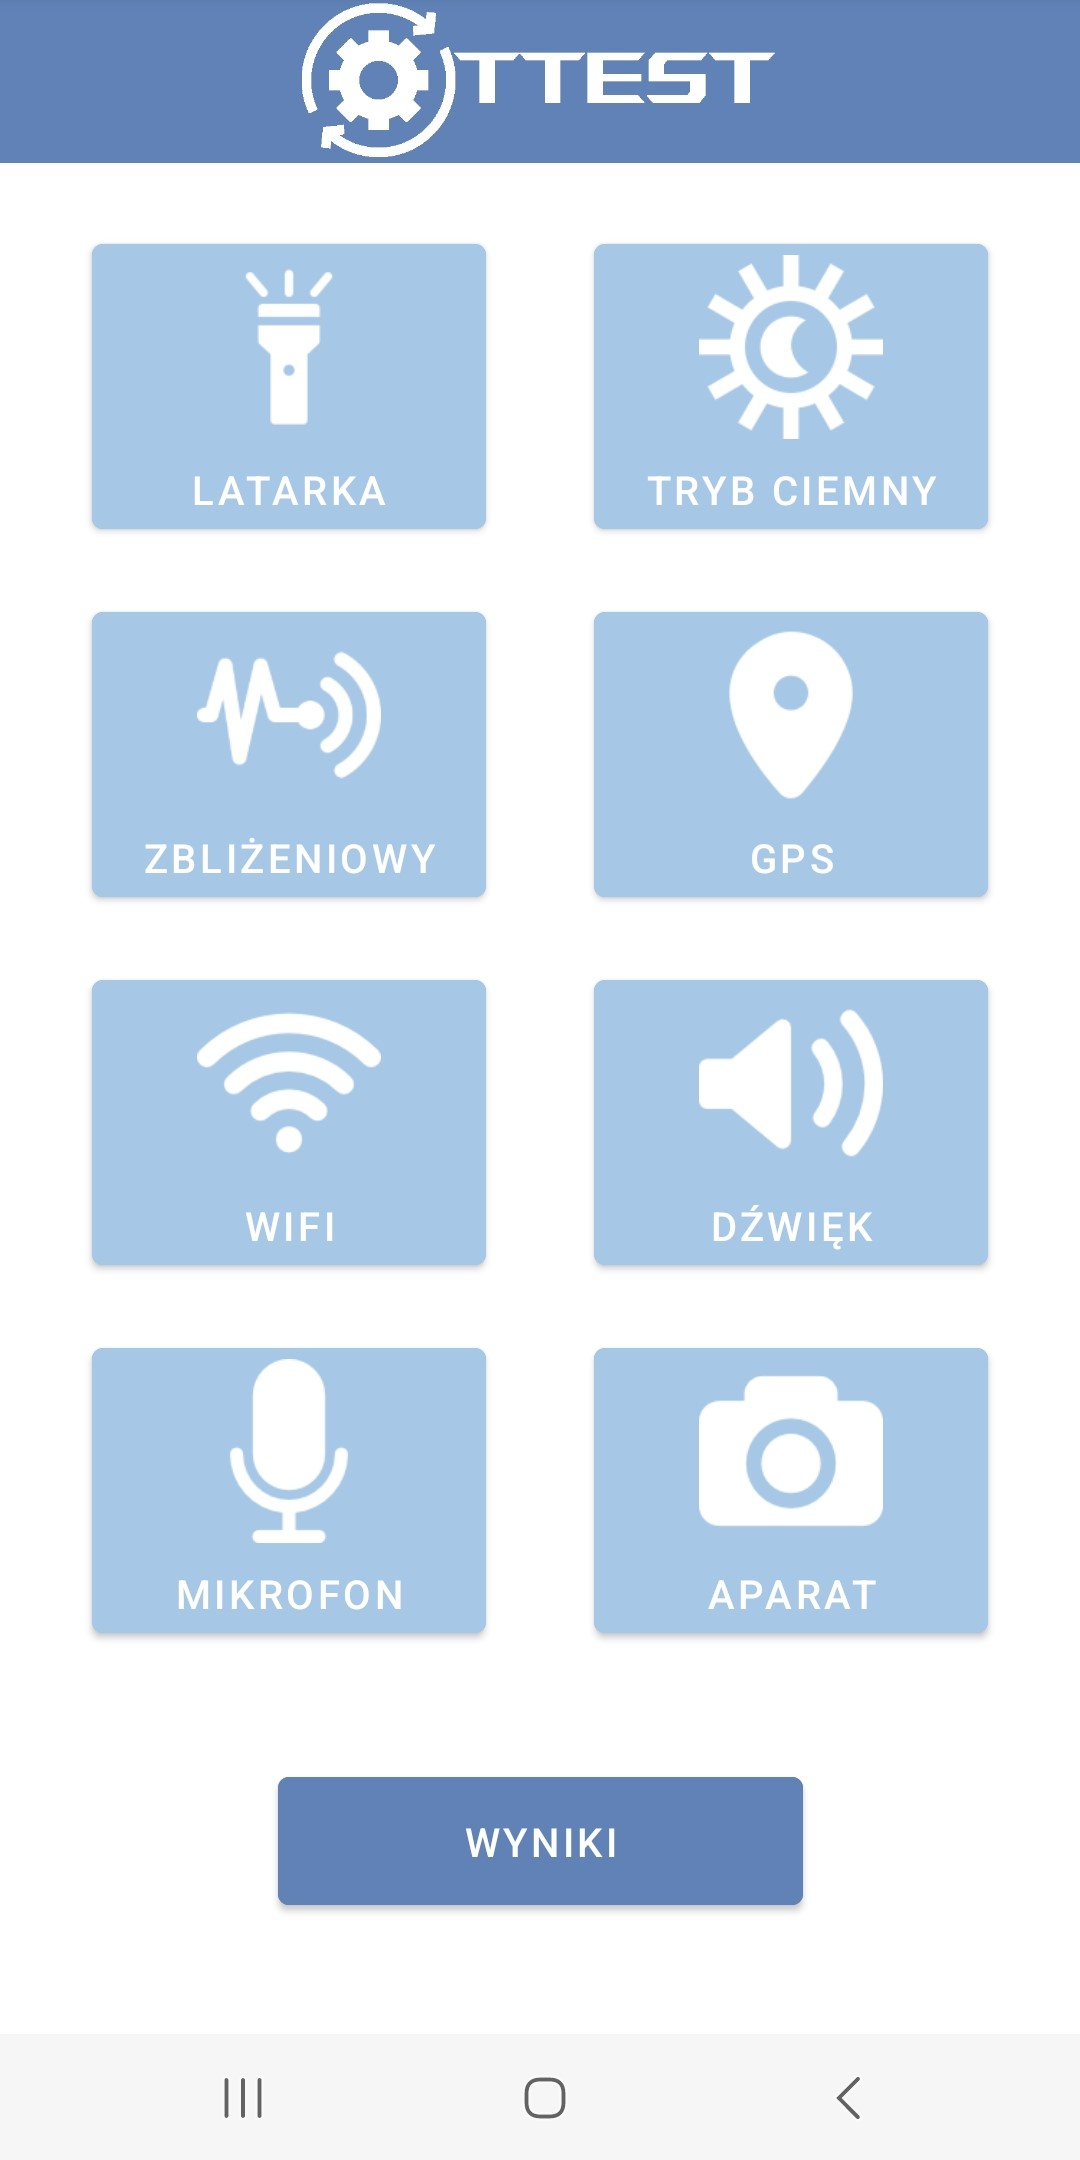
\includegraphics[angle=360, width=0.30\textwidth]{rys/punkt5/menu.jpg}
		\caption{Przebieg testowania menu}
		\label{rys:menu}
	\end{center}
\end{figure}   

\newpage


\subsection{Testowanie podsumowania}

Zadania jakie ma spełniać podsumowanie przedstawione są w tabeli \ref{tab:tablica_wyniki}. Jako "X" w kolumnie "Tak" lub "Nie", oznaczamy pomyślny lub niepomyślny przebieg poszczególnych zadań. Całość testu podsumowana jest rzutami ekranu \ref{rys:wyniki} wykonanymi podczas testowania jako potwierdzenie wykonanego testu.

\begin{tabela}
	{Testowanie podsumowania}	%opis w spisie tabel
	{Testowanie podsumowania}	%opis przy tabeli
	{
		\begin{tabular}{|c|c|c|c|} \hline
			\textbf{lp} & \textbf{Zadania do przetestowania} & \textbf{Tak} & \textbf{Nie} \\ \hline
			1 & Wyświetla się informacja o marce i modelu telefonu & X & ~ \\ \hline
			2 & W każdej grupie można wybrać tylko jeden przycisk typu radio & X & ~ \\ \hline
			3 & Po naciśnięciu na guzik pojawia się podsumowanie zaznaczaonych opcji & X & ~ \\ \hline
			4 & Pozytywne wyniki testów są wyswietlane na zielono & X & ~ \\ \hline
			5 & Negatywne wyniki testów są wyswietlane na czerwono & X & ~ \\ \hline
	\end{tabular}	}
	\label{tab:tablica_wyniki}
\end{tabela}

Obrazek \ref{rys:wyniki} przedstawia zrzuty ekranu potwierdzające pomyślny przebieg testu.

\begin{figure}[!hbt]
	\begin{center}
		
\includegraphics[angle=360, width=0.90\textwidth]{rys/punkt5/wyniki.png}
		\caption{Przebieg testowania podsumowania}
		\label{rys:wyniki}
	\end{center}
\end{figure}   

\newpage


   	\newpage
\section{Podręcznik użytkownika}  %6
%Opis jak używać programu. Mogą być z zrzut ekranu razem z opisem. 


\subsection{Wyszukiwanie i uruchomienie aplikacji Ttest} 

\hspace{0.60cm}Pierwszym krokiem jaki musimy podjąć, aby uruchomić aplikację, jest włączenie telefonu a następnie wyszukujemy po nazwie aplikację: Ttest. Powinno nam wyskoczyć okienko z nazwą i ikonką. Rysunek \ref{rys:ikona_6} przedstawia efekt po wyszukaniu aplikacji Ttest.

\begin{figure}[!hbt]
	\begin{center}
		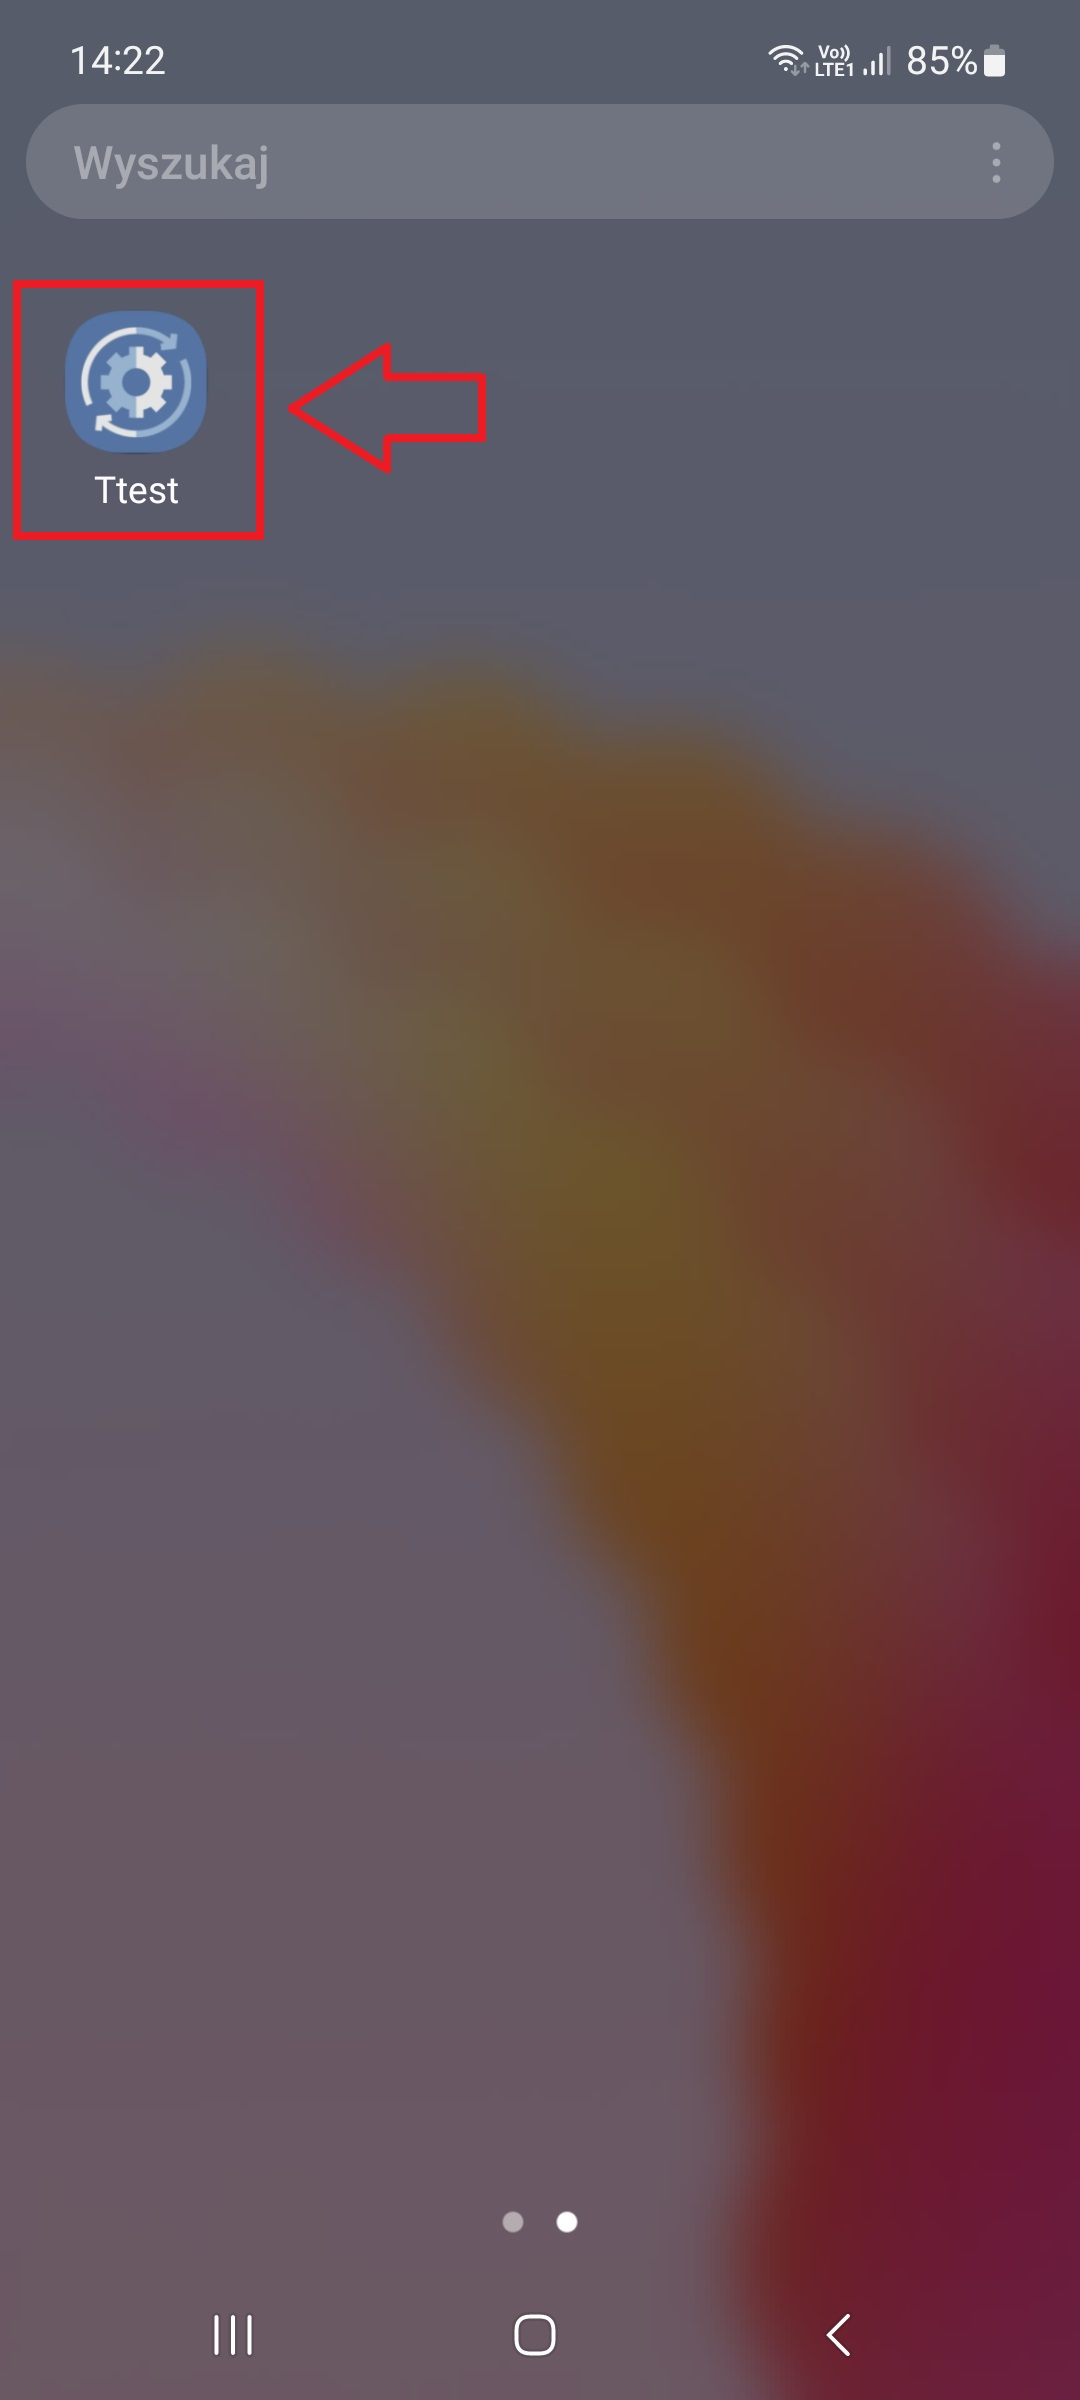
\includegraphics[angle=360, width=0.45\textwidth]{rys/punkt6/ikona.jpg}
		\caption{Wyszukiwanie aplikacji}
		\label{rys:ikona_6}
	\end{center}
\end{figure}

Gdy już odnaleźliśmy aplikację Ttest, klikamy w nią a program automatycznie przekierowuję nas do menu głównego aplikacji. 

\newpage


Menu składa się z ośmiu różnych testów. Są to testy: latarki, trybu ciemnego, czujnika zbliżeniowego, lokalizacji, wifi, dźwięku, mikrofonu oraz aparatu. Każdy jeden z testów kryję się pod przyciskiem, który został ówcześnie oznaczony odpowiednią grafiką odpowiadającą danemu testowi oraz podpisem znajdującym się u dołu obrazka. Na samym dole pod testami znajduję się przycisk z napisem "Wyniki", jest to swego rodzaju podsumowanie działalności wszystkich testów znajdujących się w aplikacji. Rysunek \ref{rys:menu1} prezentuje widok menu głównego.

\begin{figure}[!hbt]
	\begin{center}
		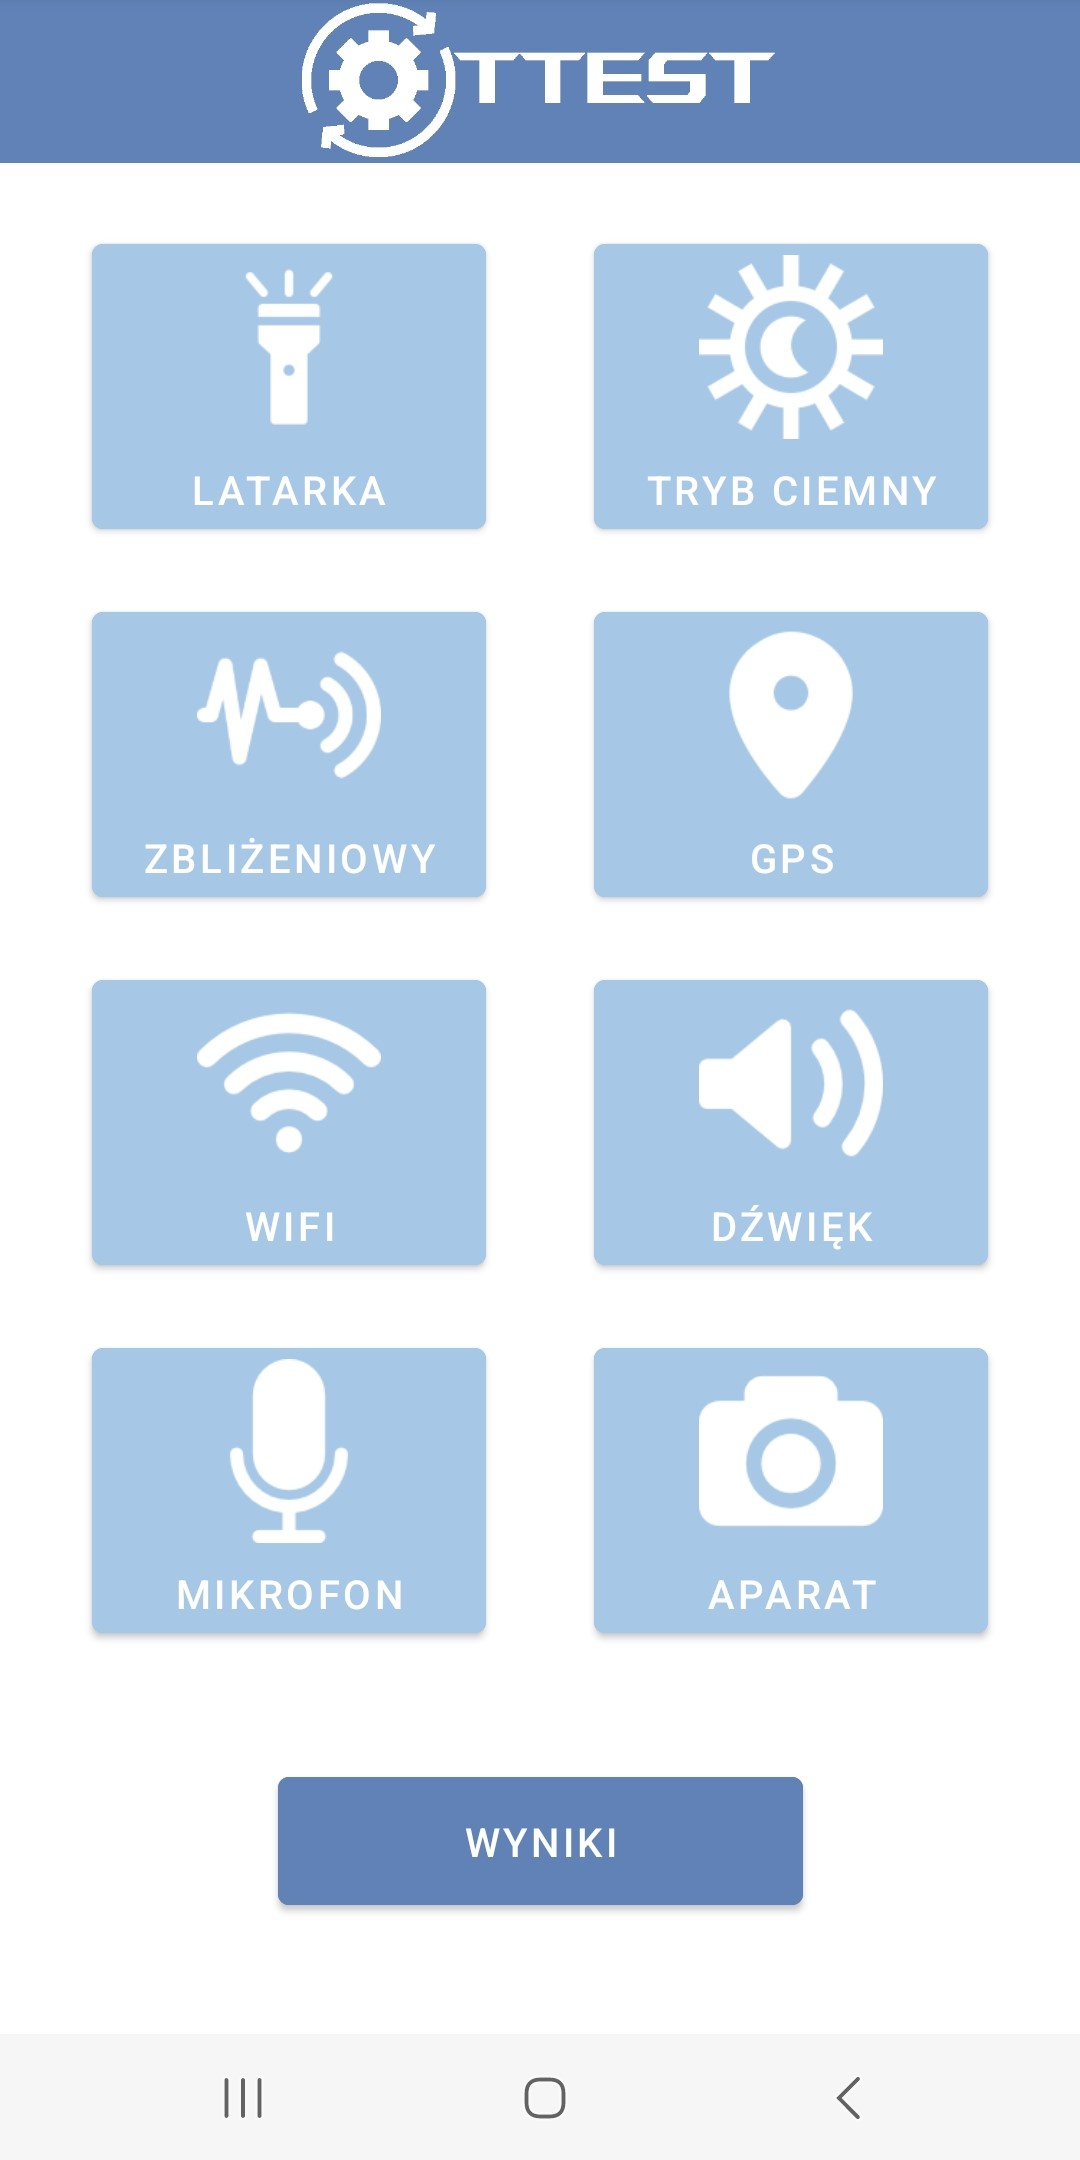
\includegraphics[angle=360, width=0.45\textwidth]{rys/punkt6/menu1.jpg}
		\caption{Menu główne}
		\label{rys:menu1}
	\end{center}
\end{figure}

\newpage


\subsection{Test latarki} 

\hspace{0.60cm}Aby uruchomić latarkę w menu głównego wybieramy i klikamy na ikonkę latarki, która znajduję się na samej górze po lewej stronie. Rysunek \ref{rys:latarka1} ukazuję miejsce które należy wybrać. 

\begin{figure}[!hbt]
	\begin{center}
		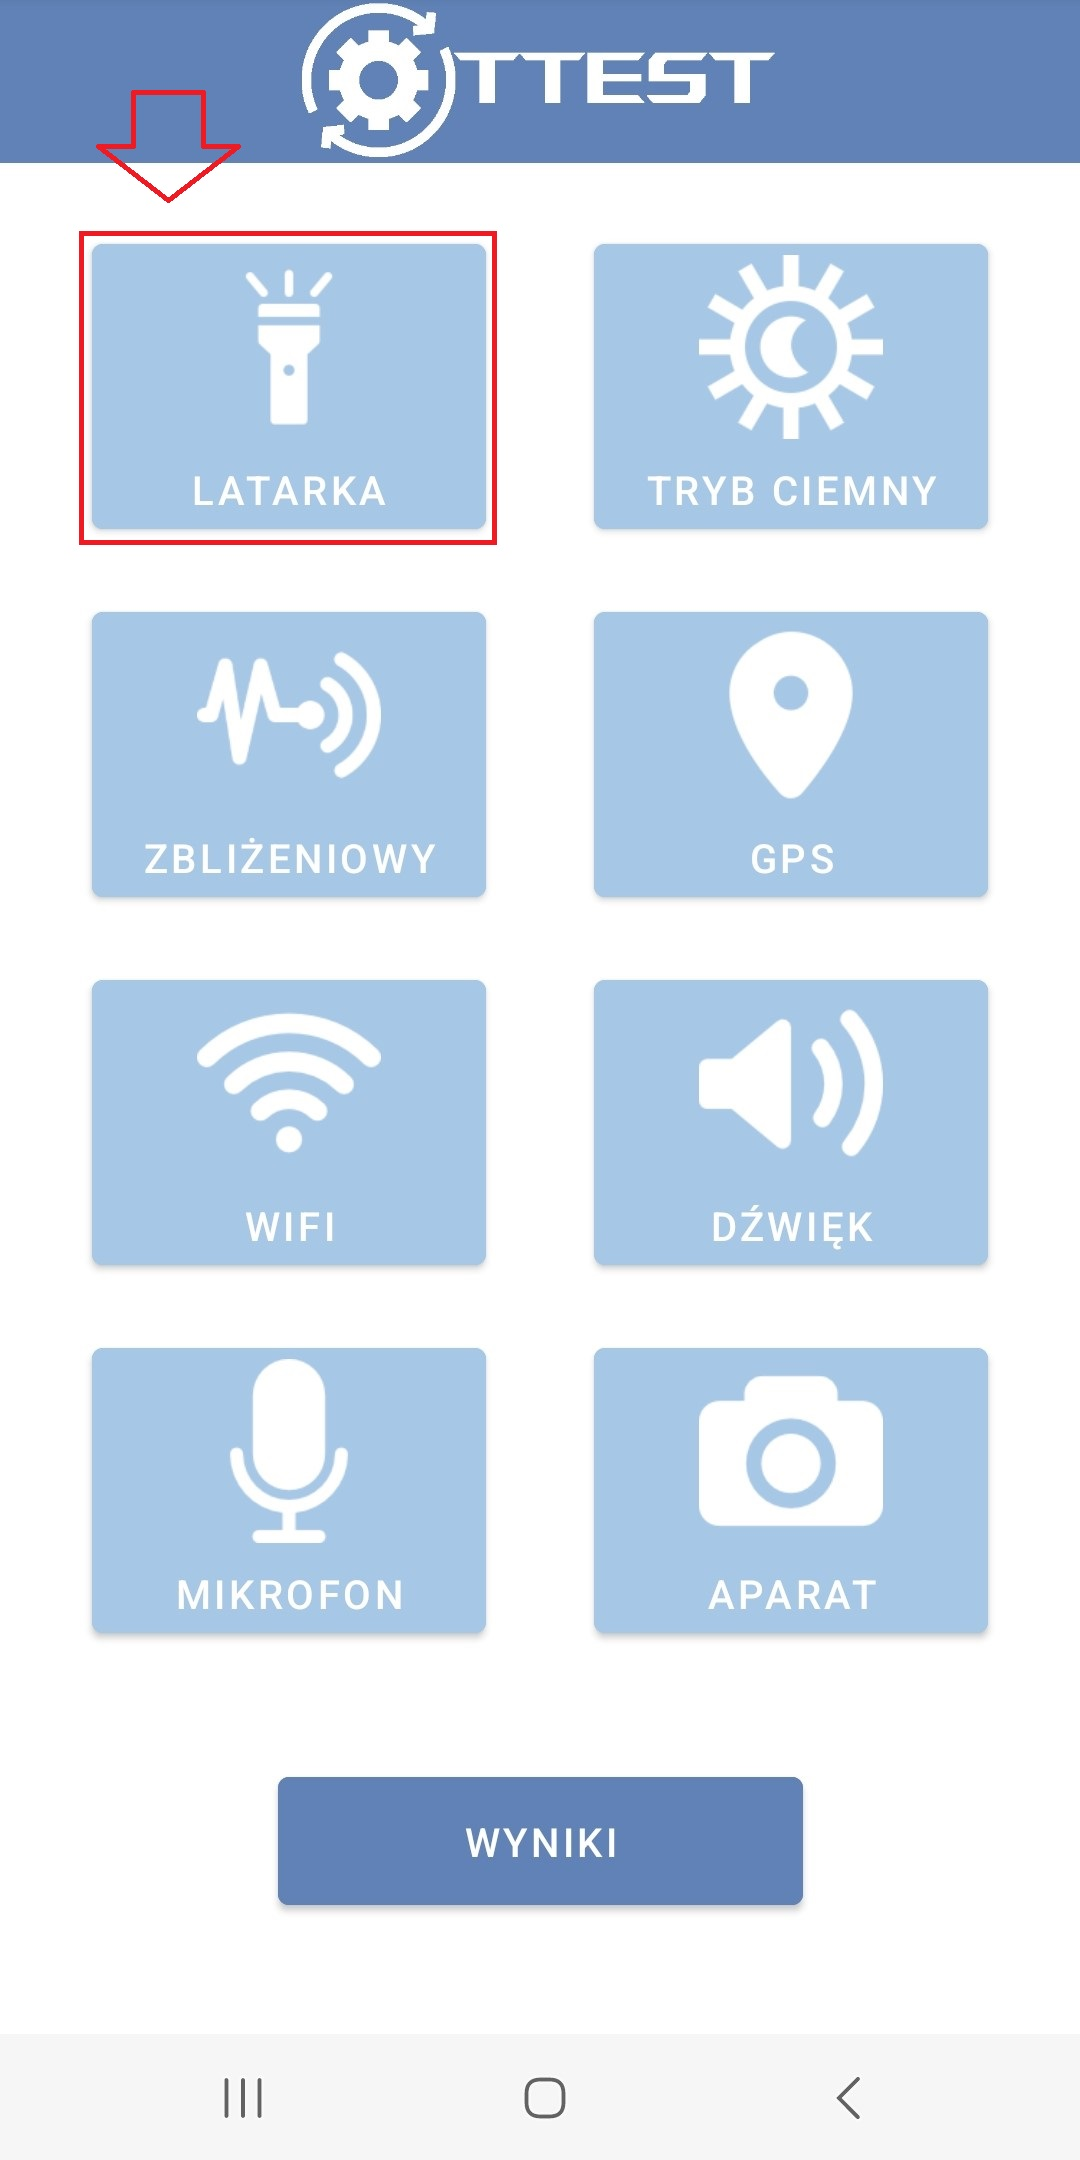
\includegraphics[angle=360, width=0.45\textwidth]{rys/punkt6/latarka1.jpg}
		\caption{Wybór latarki}
		\label{rys:latarka1}
	\end{center}
\end{figure}

Następnie aplikacja przekierowuje nas do testu latarki. Pojawia się okienko a na środku znajduję się grafika przedstawiająca latarkę.
Gdy naciśniemy na latarkę jej kolor zmieni się z szarego na zielony, oznacza to że test przeszedł pomyślnie i latarka włączyła się. Oprócz zielonego koloru pod latarką wyświetla się komunikat informujący nas o tym że latarka została włączona. Rysunek \ref{rys:latarka2} przedstawia zrzuty ekranu potwierdzające pomyślny przebieg testu.
\newpage


\begin{figure}[!hbt]
	\begin{center}
		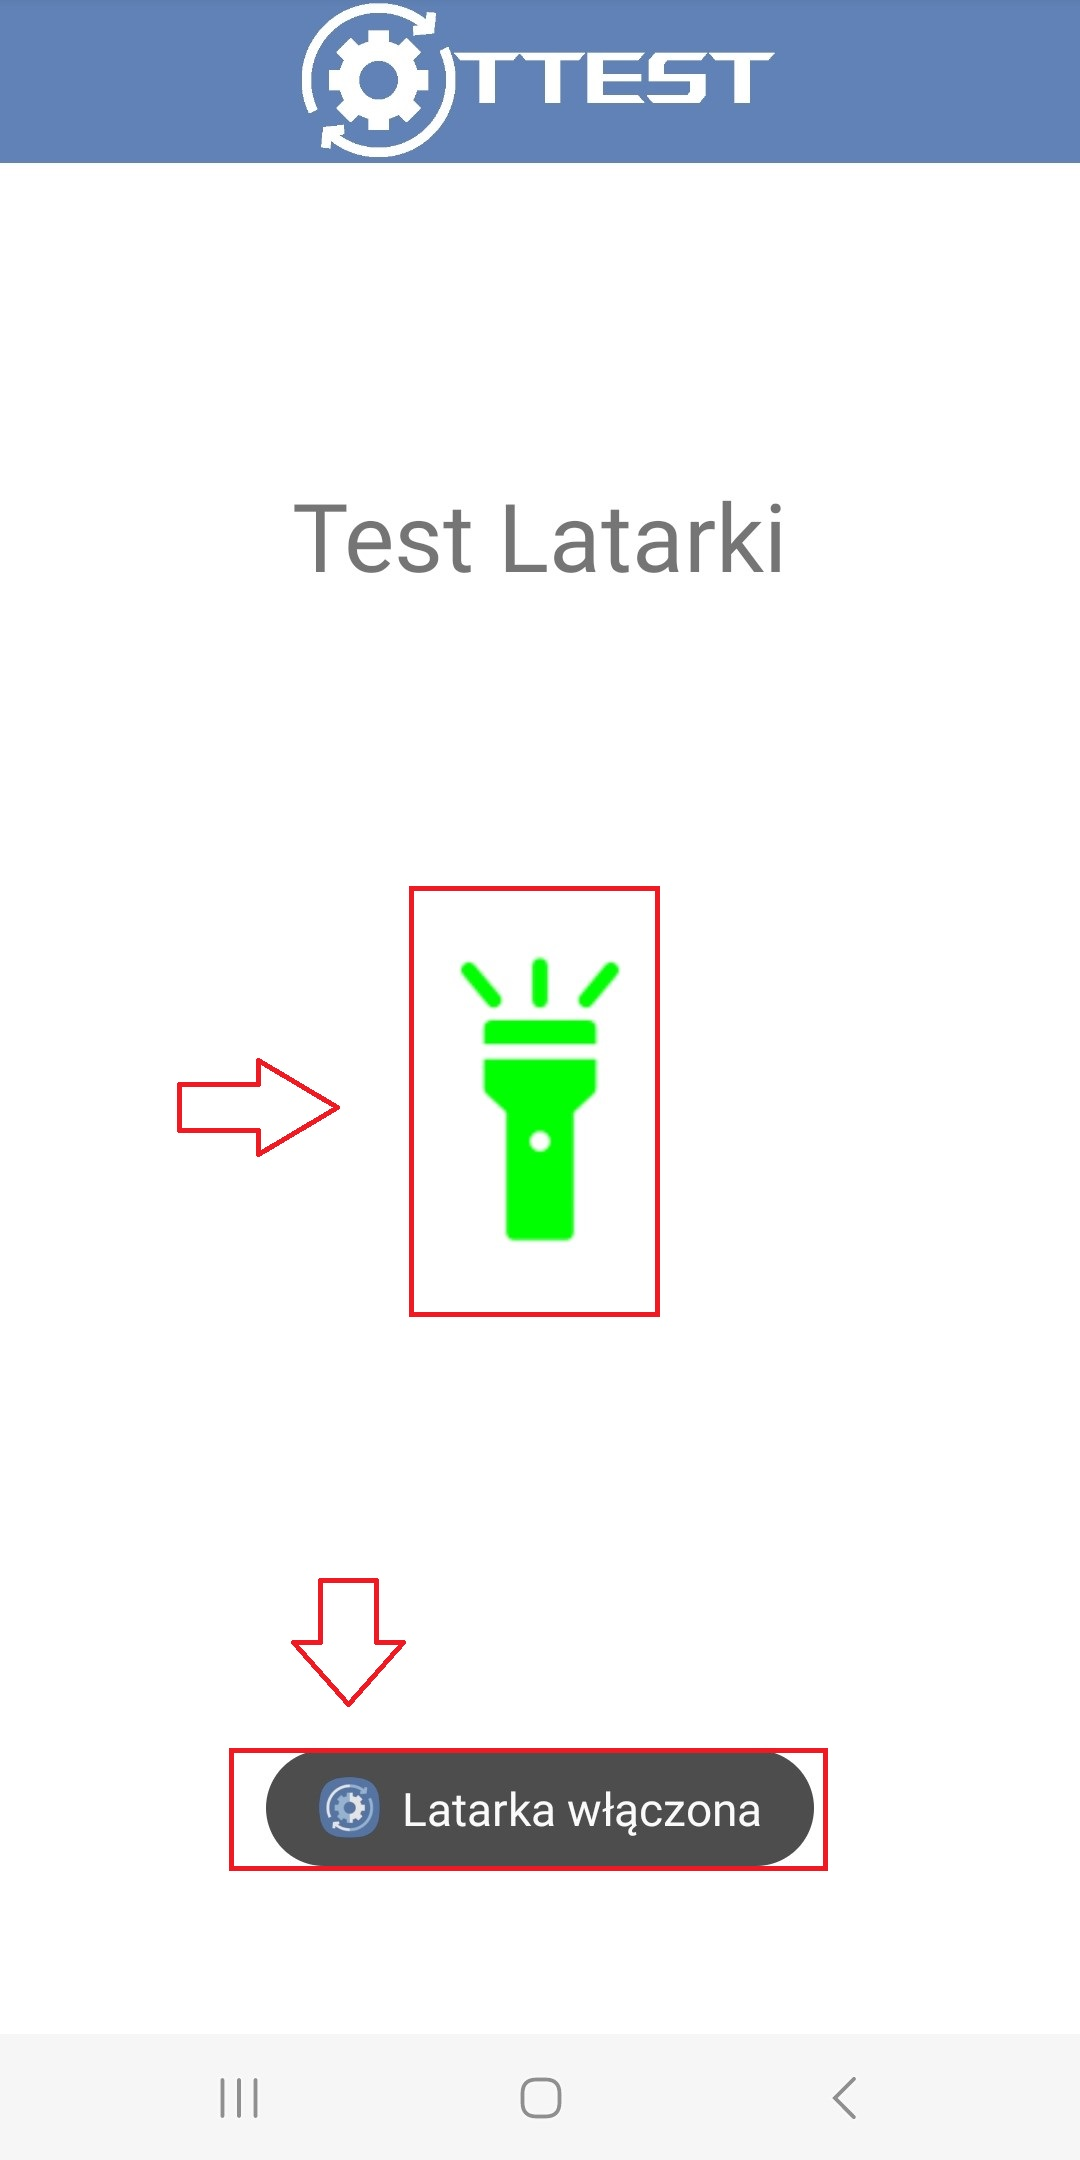
\includegraphics[angle=360, width=0.31\textwidth]{rys/punkt6/latarka2.jpg}
		\caption{Działanie latarki}
		\label{rys:latarka2}
	\end{center}
\end{figure}

Analogicznie jak w przypadku włączenia gdy naciśniemy na latarkę kolejny raz, test zostanie przerwany, latarka wyłączy się i zmieni kolor z zielonego na czerwony. Rysunek \ref{rys:latarka3} przedstawia wyłączoną latarkę.

\begin{figure}[!hbt]
	\begin{center}
		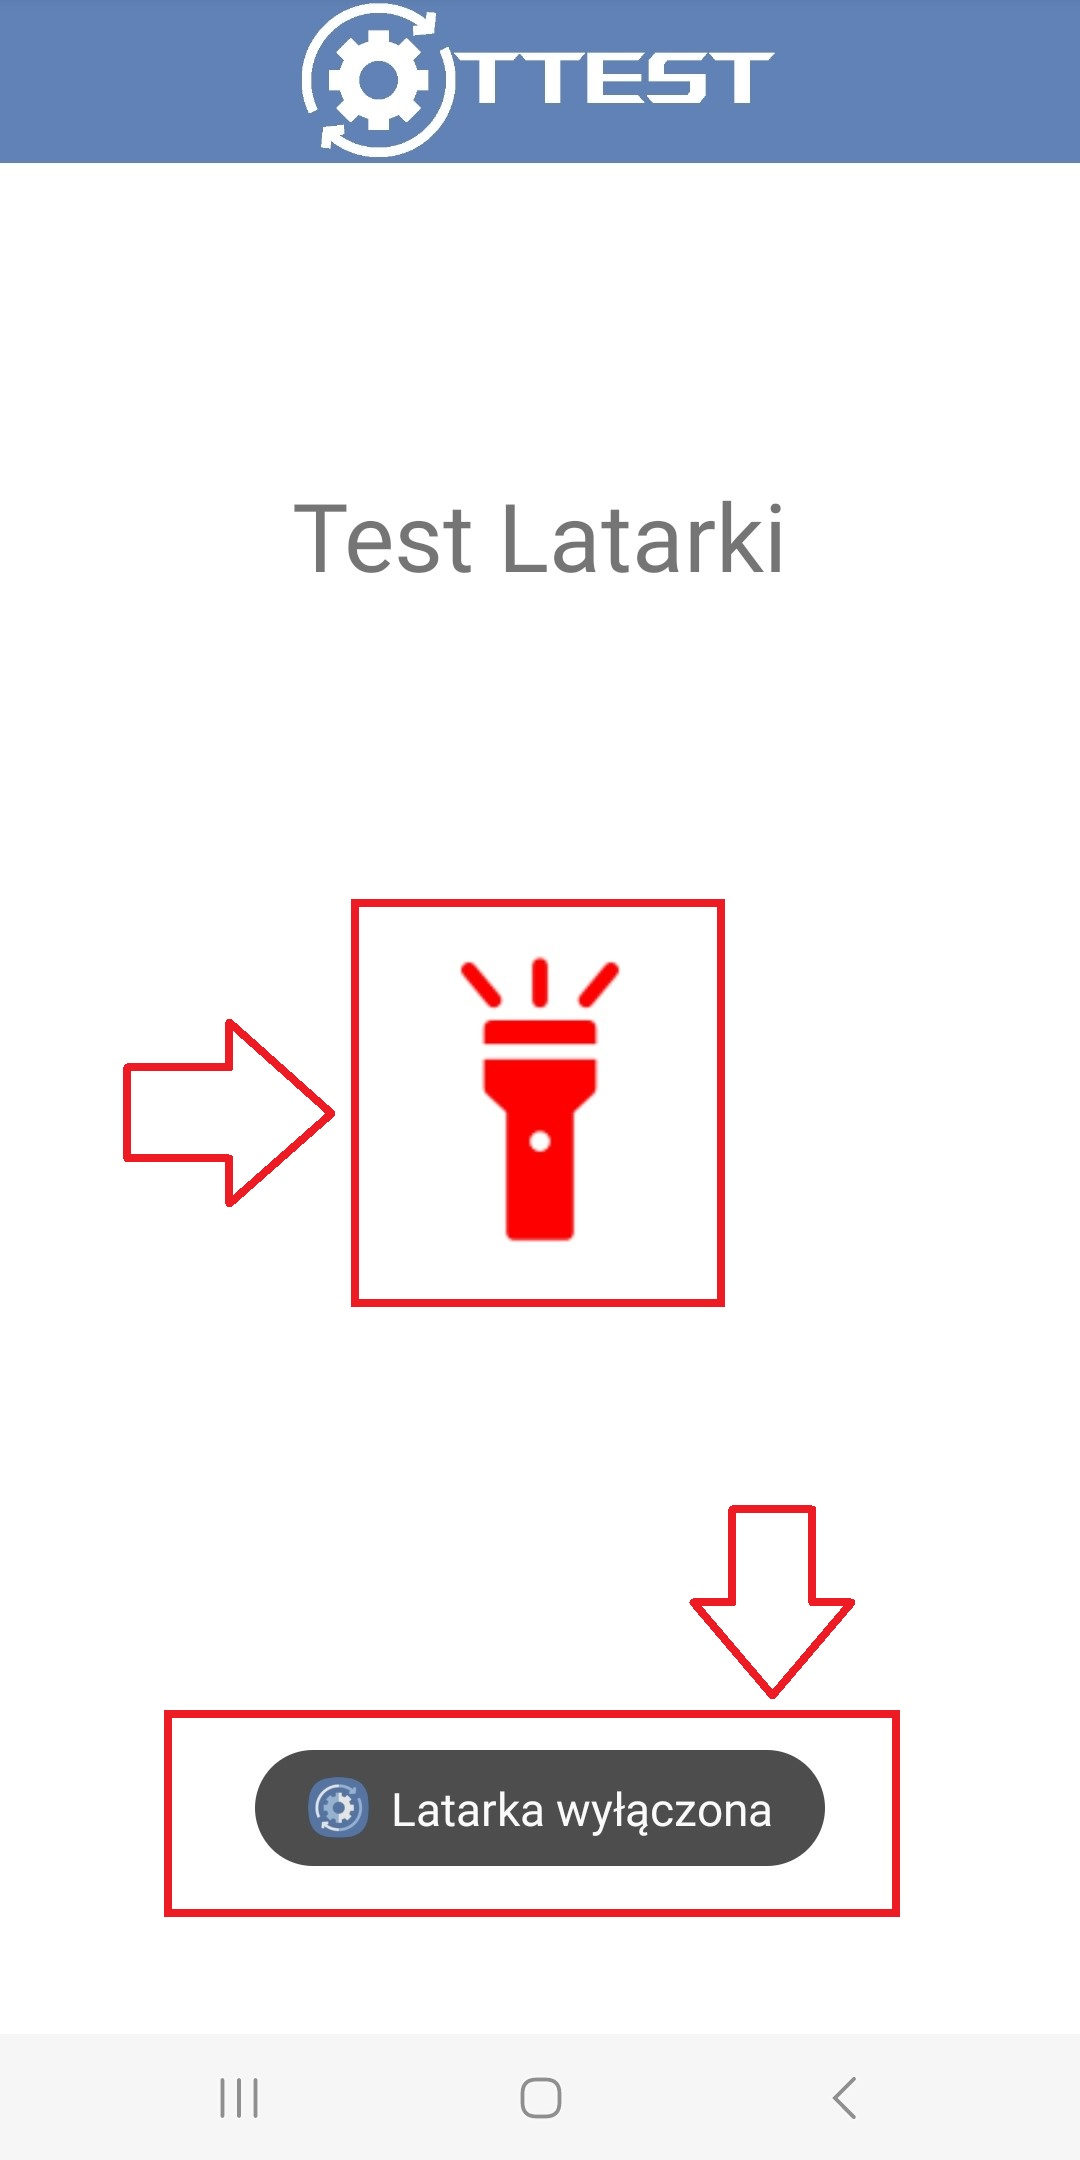
\includegraphics[angle=360, width=0.31\textwidth]{rys/punkt6/latarka3.jpg}
		\caption{Latarka wyłączona}
		\label{rys:latarka3}
	\end{center}
\end{figure}

\newpage


\subsection{Test trybu ciemnego}

\hspace{0.60cm}Aby uruchomić tryb ciemny musimy na panelu głównym wybrać i kliknąć w ikonkę który znajduję się na samej górze po prawej stronie. Rysunek \ref{rys:menu2} obrazuje miejsce które musimy wybrać i kliknąć aby przejść do testu.

\begin{figure}[!hbt]
	\begin{center}
		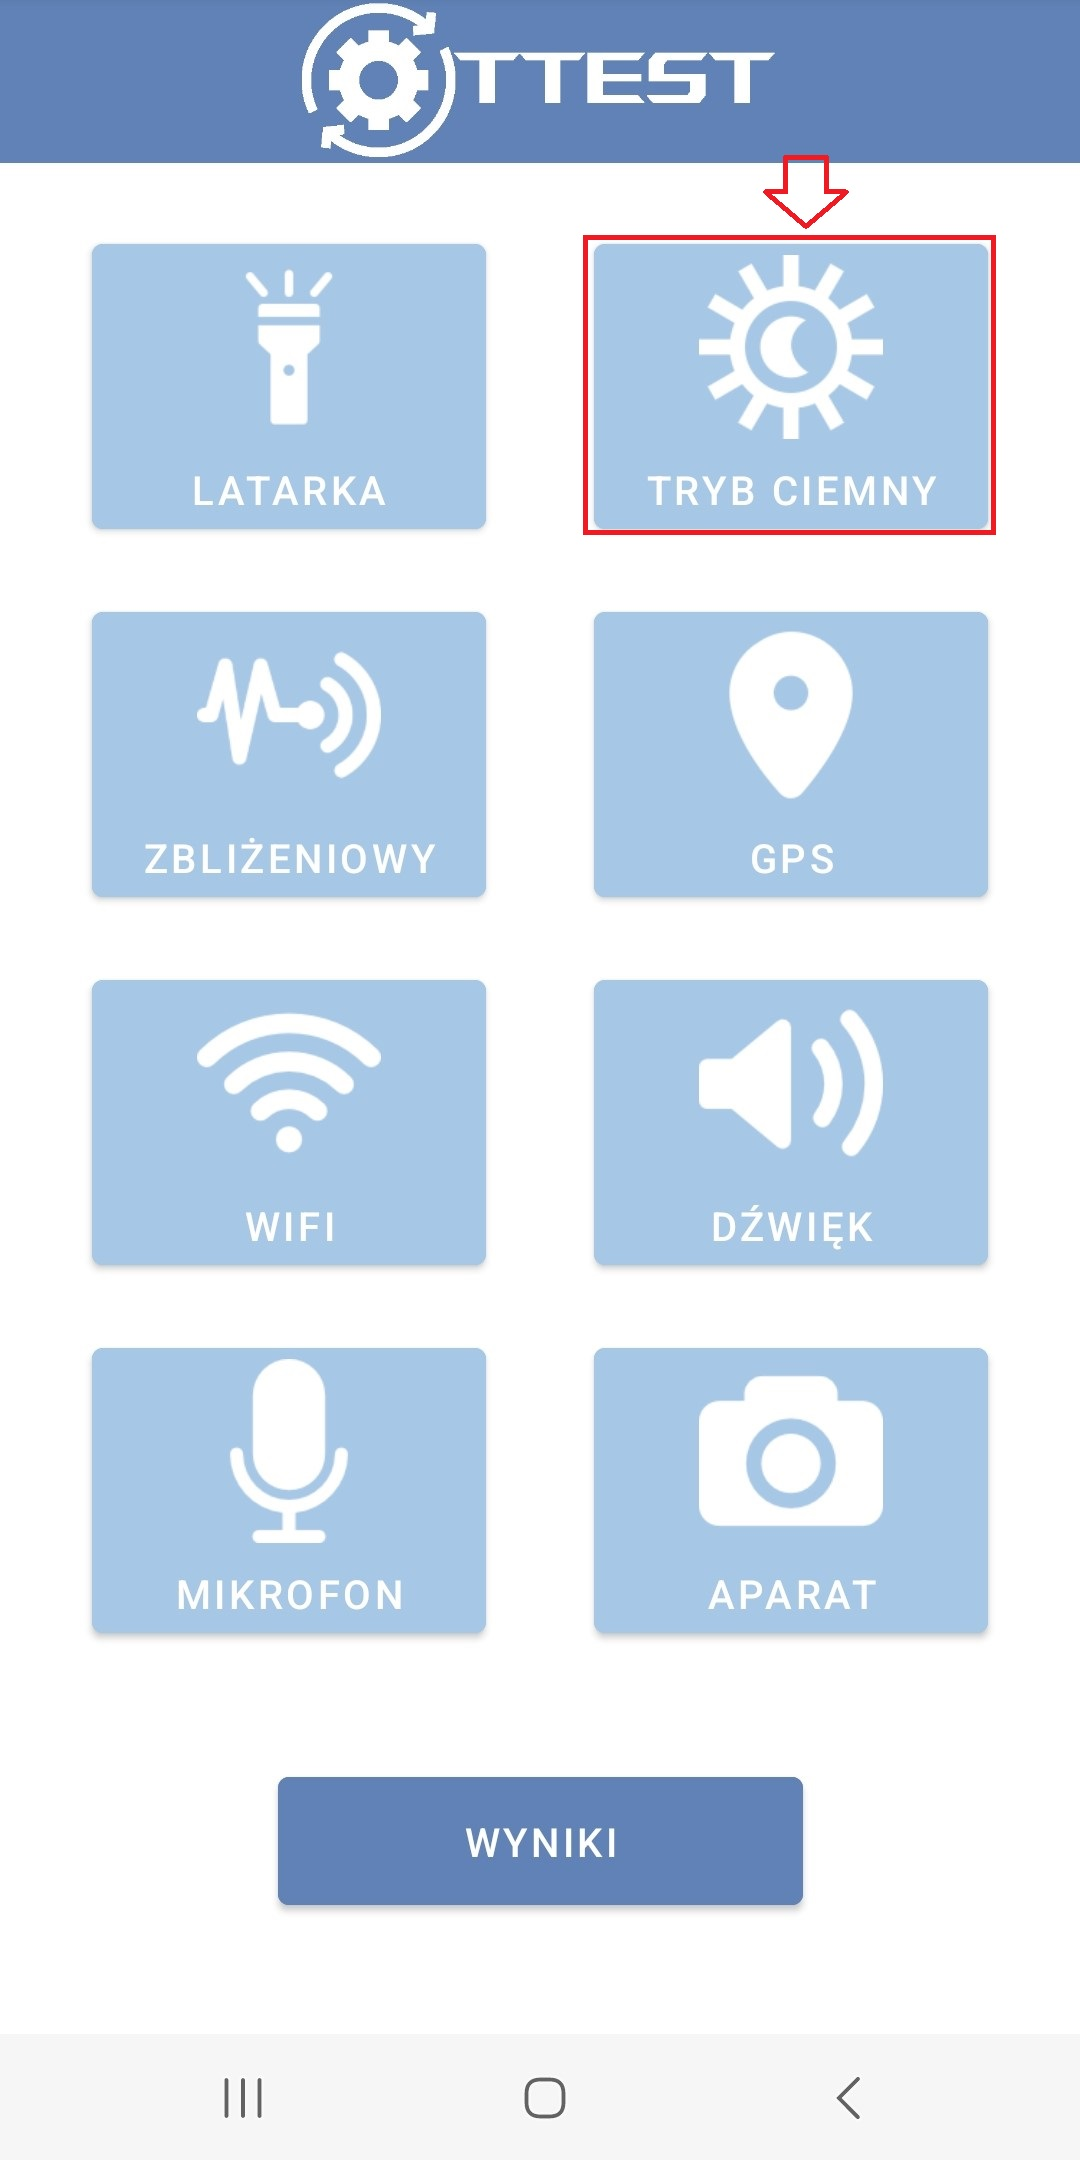
\includegraphics[angle=360, width=0.45\textwidth]{rys/punkt6/menu2.jpg}
		\caption{Wybór trybu ciemnego}
		\label{rys:menu2}
	\end{center}
\end{figure}

Następnie aplikacja przekierowuje nas do okienka testowego. Na środku znajduję się grafika, która podobnie jak w przypadku latarki zmienia kolory z zieloneg na czerwony, lub odwrotnie w zależności czy tryb zostanie włączony lub wyłączony. Jeżeli klikniemy na ikonkę a jej kolor zmieni się na zielony oznacza to że test przeszedł pomyślnie, co więcej ekran zmieni kolor z białego na czarny a pod grafiką dodatkowo pojawia się informacja o tym że tryb ciemny został uruchomiony. Rysunek \ref{rys:tryb ciemny} przedstawia uruchomienie trybu ciemnego.

\newpage


\begin{figure}[!hbt]
	\begin{center}
		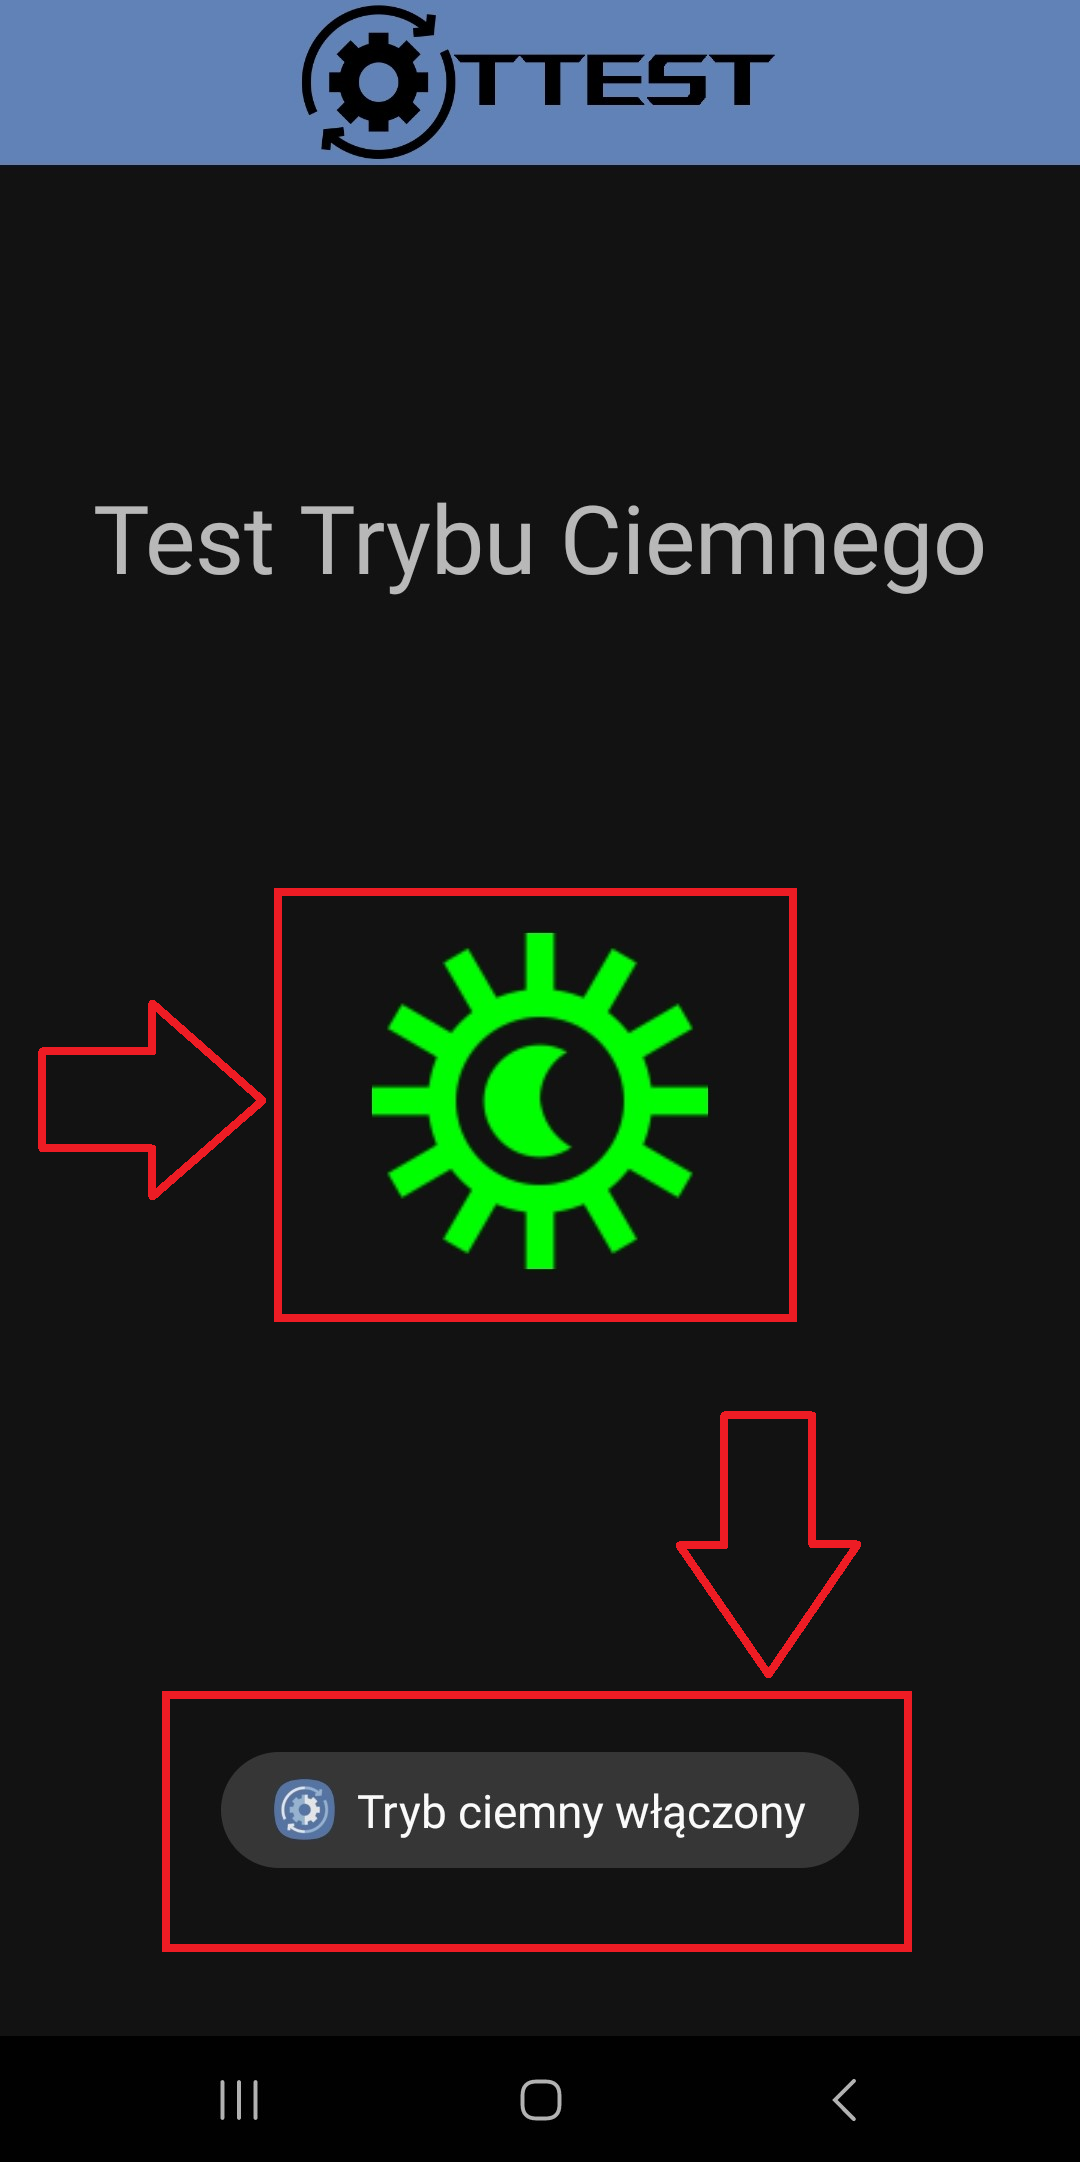
\includegraphics[angle=360, width=0.31\textwidth]{rys/punkt6/tryb ciemny.png}
		\caption{Działanie trybu ciemnego}
		\label{rys:tryb ciemny}
	\end{center}
\end{figure}

Po kliknięciu ponownie na środkowy przycisk tryb ciemny zostaje wyłączony, kolor ikonki zmienia się na czerwony, a komunikat u dołu informuje nas o wyłączeniu trybu ciemnego. Rysunek \ref{rys:tryb ciemny1} przedstawia wyłączenie trybu ciemnego. 

\begin{figure}[!hbt]
	\begin{center}
		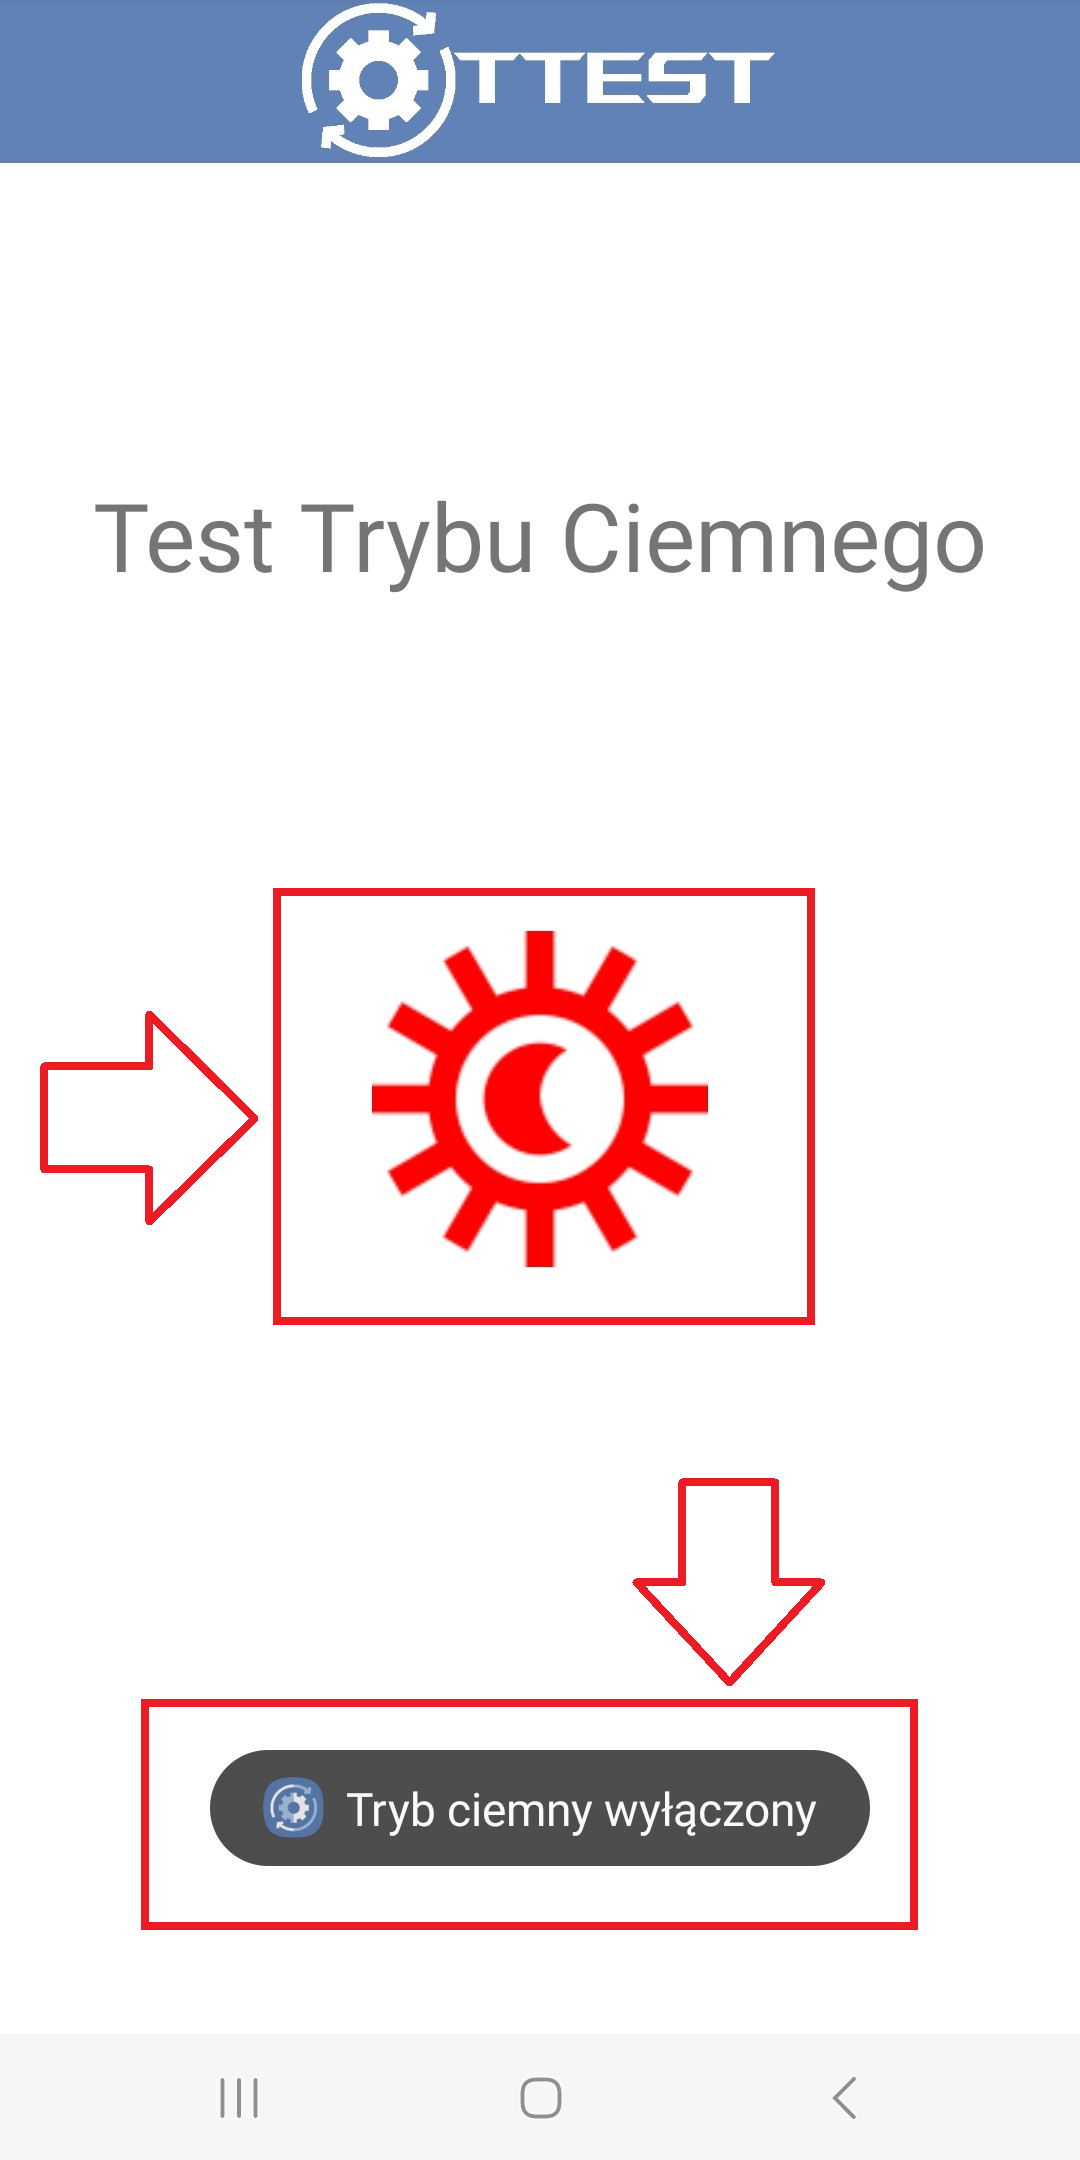
\includegraphics[angle=360, width=0.31\textwidth]{rys/punkt6/tryb ciemny1.png}
		\caption{Wyłączenie trybu ciemnego}
		\label{rys:tryb ciemny1}
	\end{center}
\end{figure}

\newpage


\subsection{Test czujnika zbliżeniowego}

\hspace{0.60cm}Aby uruchomić czujnik zbliżeniowy musimy w menu wybrać i kliknąć w ikonkę który znajduję się na pod ikonką latarki. Rysunek \ref{rys:menu3} obrazuje miejsce, które musimy wybrać i kliknąć aby przejść do testu.

\begin{figure}[!hbt]
	\begin{center}
		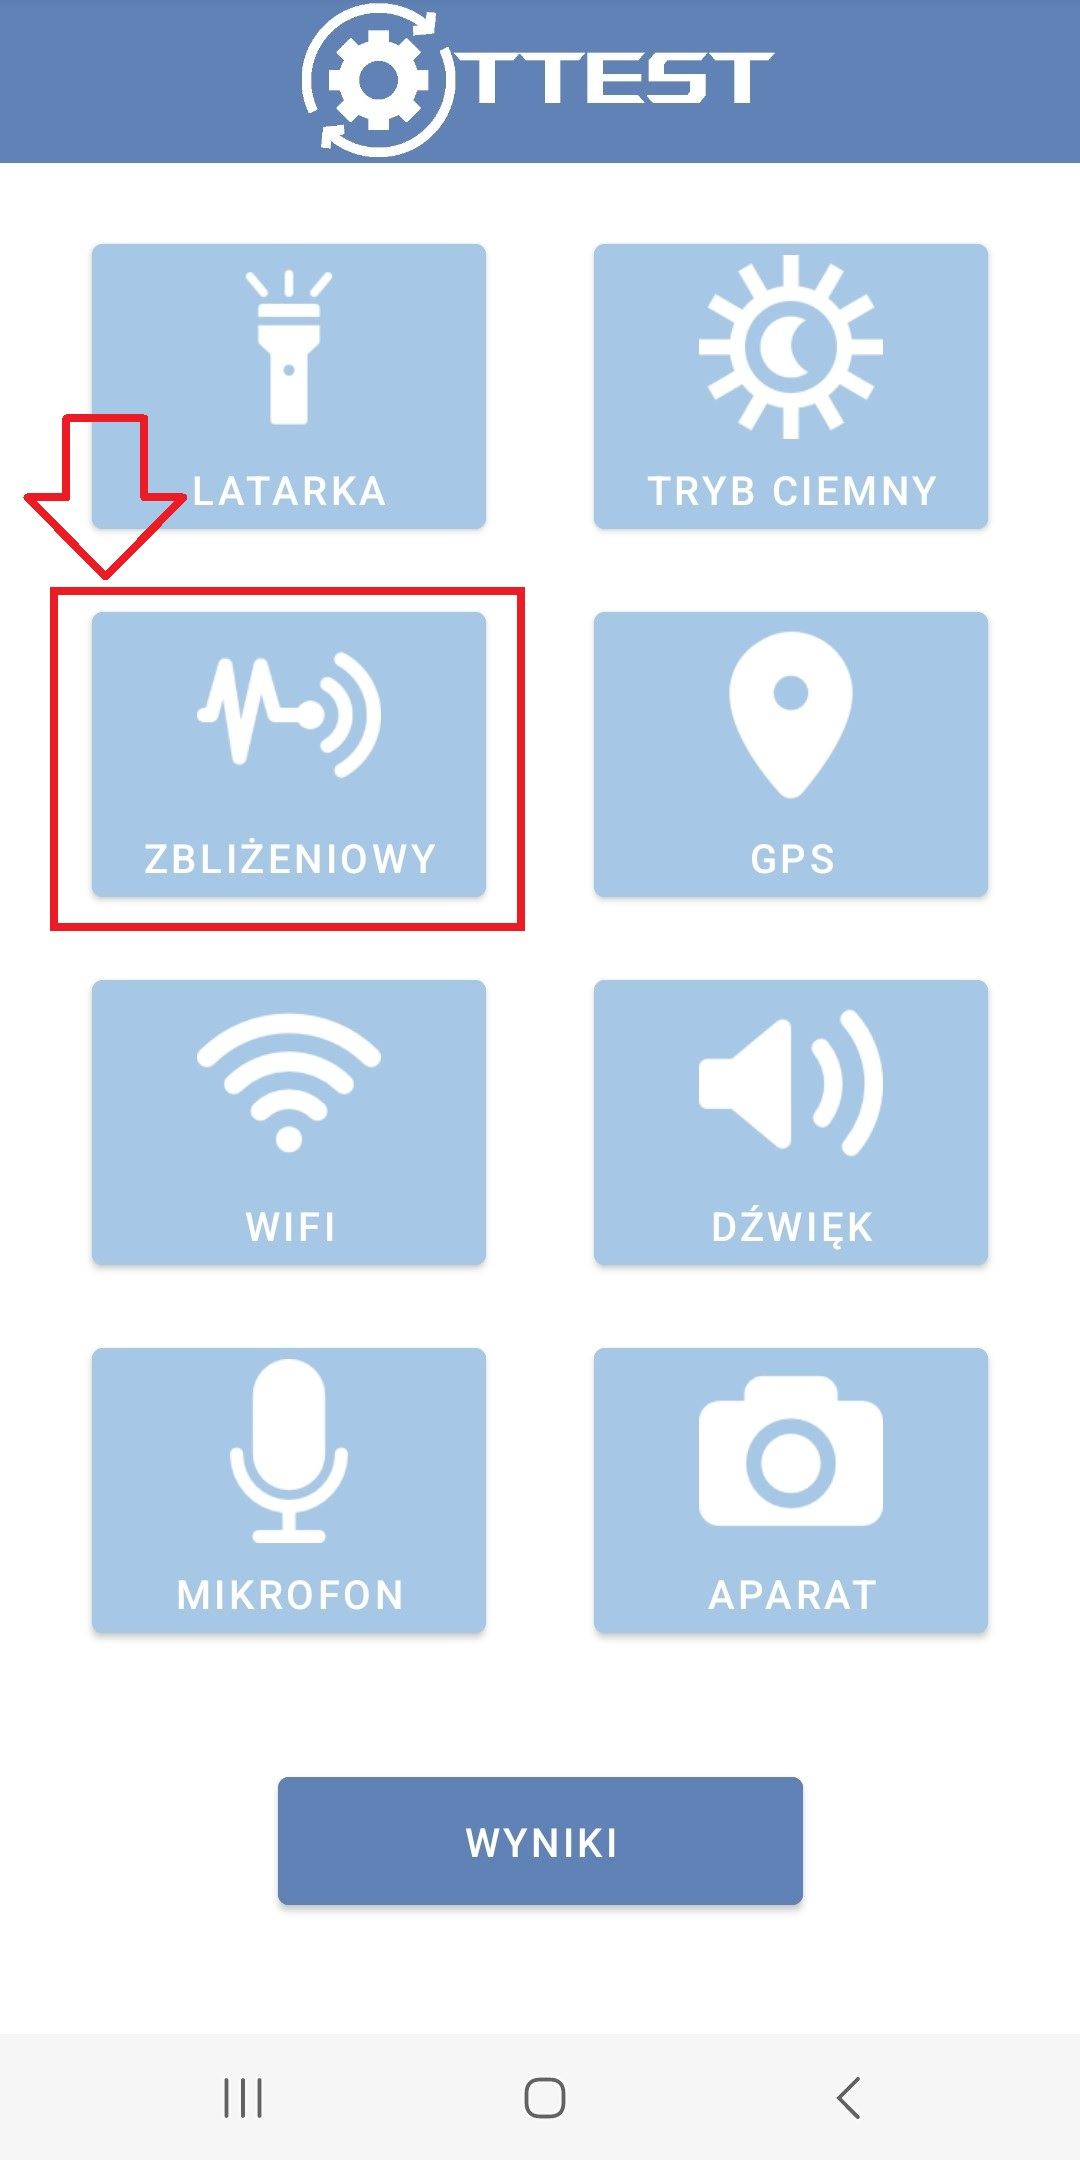
\includegraphics[angle=360, width=0.45\textwidth]{rys/punkt6/menu3.jpg}
		\caption{Lokalizacja czujnika zbliżeniowego}
		\label{rys:menu3}
	\end{center}
\end{figure}

Po przejściu do strony z testem wyświetla nam się informacja aby przyłożyć obiekt do czujnika. Rysunek \ref{rys:czujnik zbliżeniowy} prezentuje stronę z testem czujnika. \\

Czujnik znajduję się przy przedniej kamerce telefonu wystarczy przyłożyć palec a informacja zmienia się i zaczyna wyświetlać komunikat o treści : Przy czujniku jest obiekt. Jeżeli odsuniemy palec od czujnika informacja ponownie zacznie wyświetlać komunikat o treści: Przyłóż obiekt do czujnika.

\newpage


\begin{figure}[!hbt]
	\begin{center}
		\includegraphics[angle=360, width=0.32\textwidth]{rys/punkt6/czujnik zbliżeniowy}
		\caption{Strona testowa czujnika zbliżeniowego}
		\label{rys:czujnik zbliżeniowy}
	\end{center}
\end{figure}

Rysunek \ref{rys:czujnik zbliżeniowy1} przedstawia zrzut ekranu potwierdzający pomyślny przebieg testu.

\begin{figure}[!hbt]
	\begin{center}
		\includegraphics[angle=360, width=0.32\textwidth]{rys/punkt6/czujnik zbliżeniowy1}
		\caption{Działanie czujnika zbliżeniowego}
		\label{rys:czujnik zbliżeniowy1}
	\end{center}
\end{figure}

\newpage


\subsection{Test GPS}

\hspace{0.60cm}Aby uruchomić test GPS'a musimy w menu wybrać i kliknąć w przycisk który znajduję się na pod ikonką trybu ciemnego. Rysunek \ref{rys:menu4} obrazuje miejsce, które musimy wybrać i kliknąć aby przejść do testu.

\begin{figure}[!hbt]
	\begin{center}
		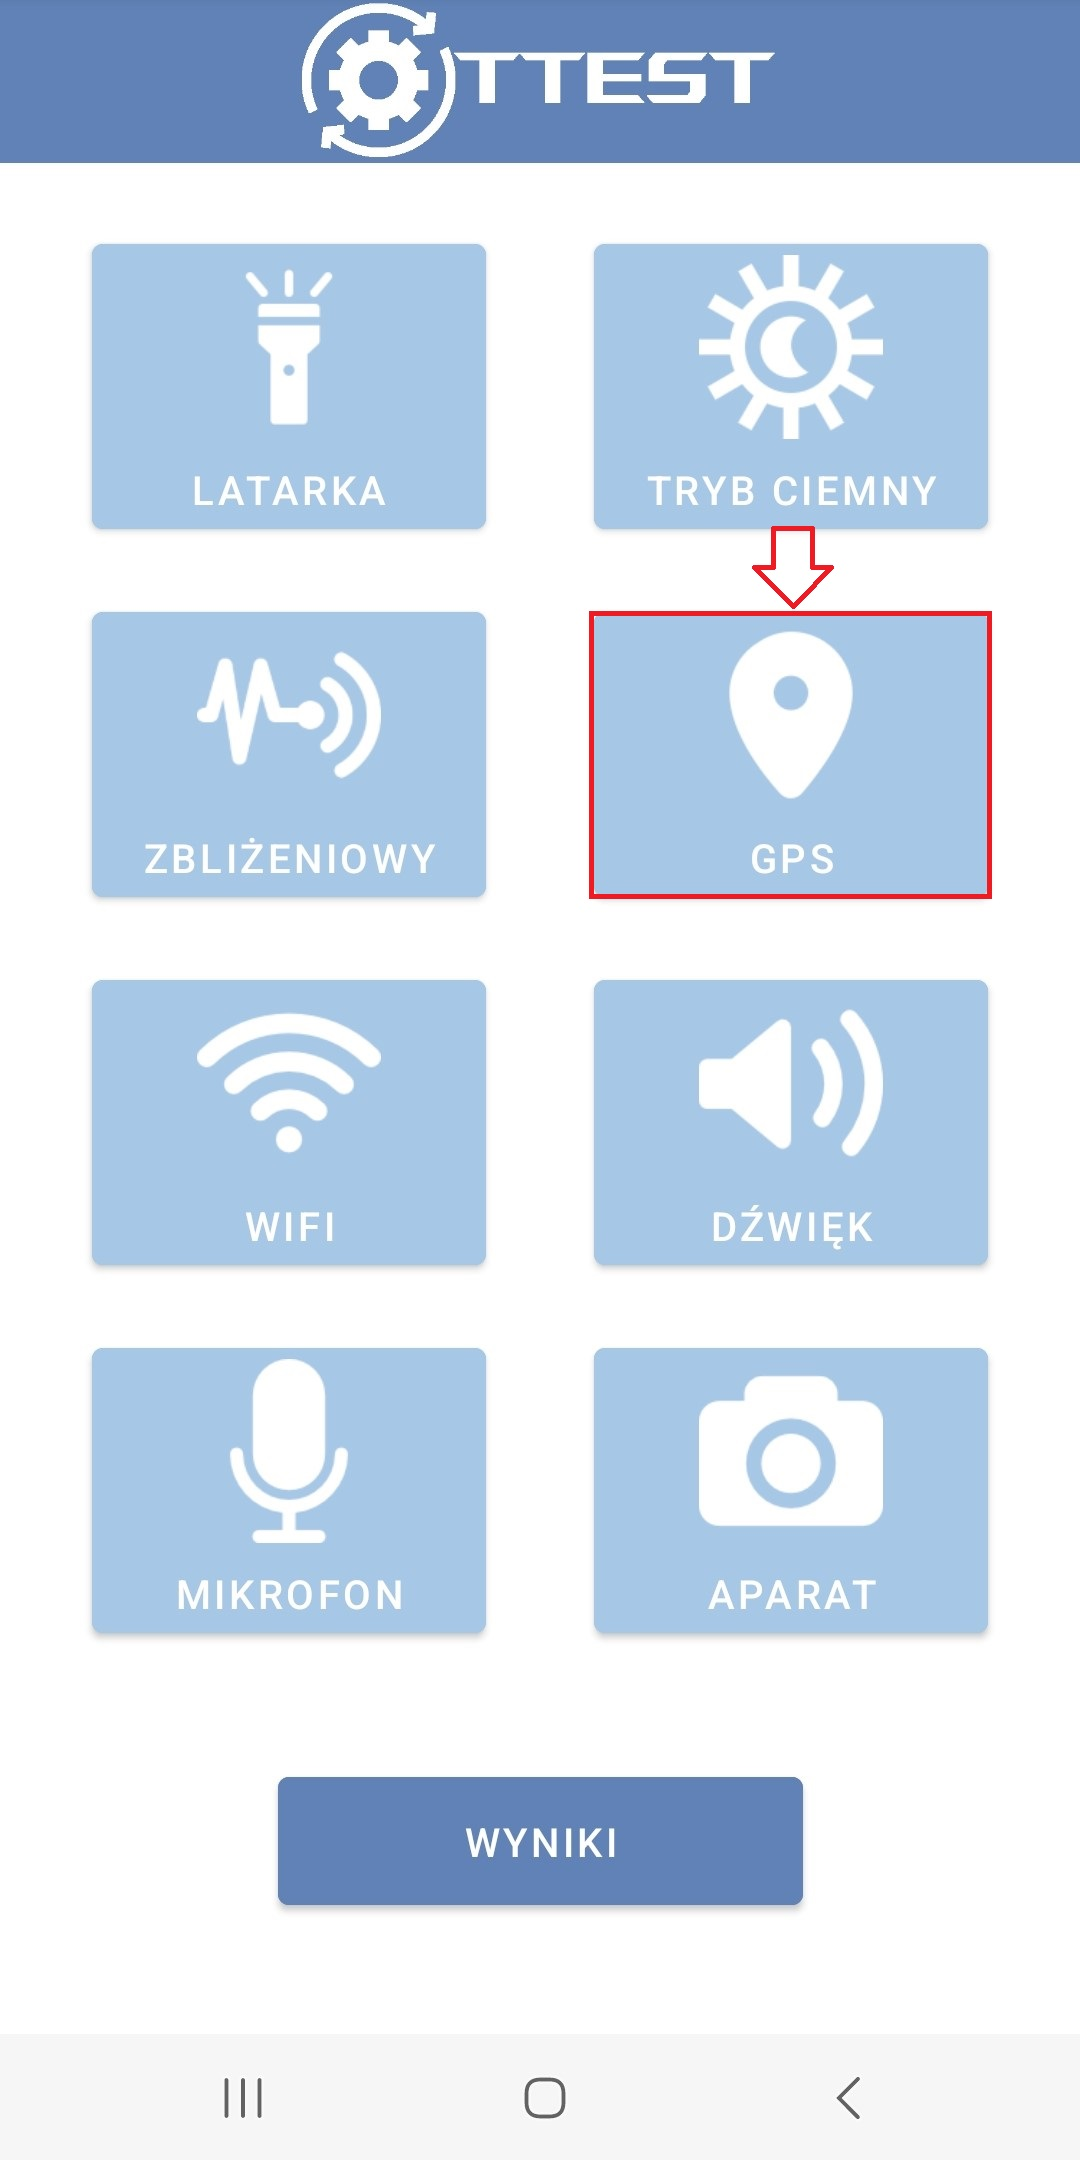
\includegraphics[angle=360, width=0.45\textwidth]{rys/punkt6/menu4}
		\caption{Wybór GPS'a}
		\label{rys:menu4}
	\end{center}
\end{figure}

Po przejściu do strony z testem na środku ekranu  wyświetla nam się przycisk, którego celem jest wyszukanie naszej aktualnej lokalizacji. Rysunek \ref{rys:gps} prezentuje stronę z testem lokalizacji. \\

Gdy klikniemy na przycisk po krótkiej chwili wyświetli nam się dokładna lokalizacja w której się znajdujemy co więcej pojawi się również kod pocztowy i kraj w którym się znajdujemy. Oprócz wyżej wymienionych informacji u dołu pod lokalizacją zostaje wyświetlona w formie pop-up'u szerokość i długość geograficzna.

\newpage

\begin{figure}[!hbt]
	\begin{center}
		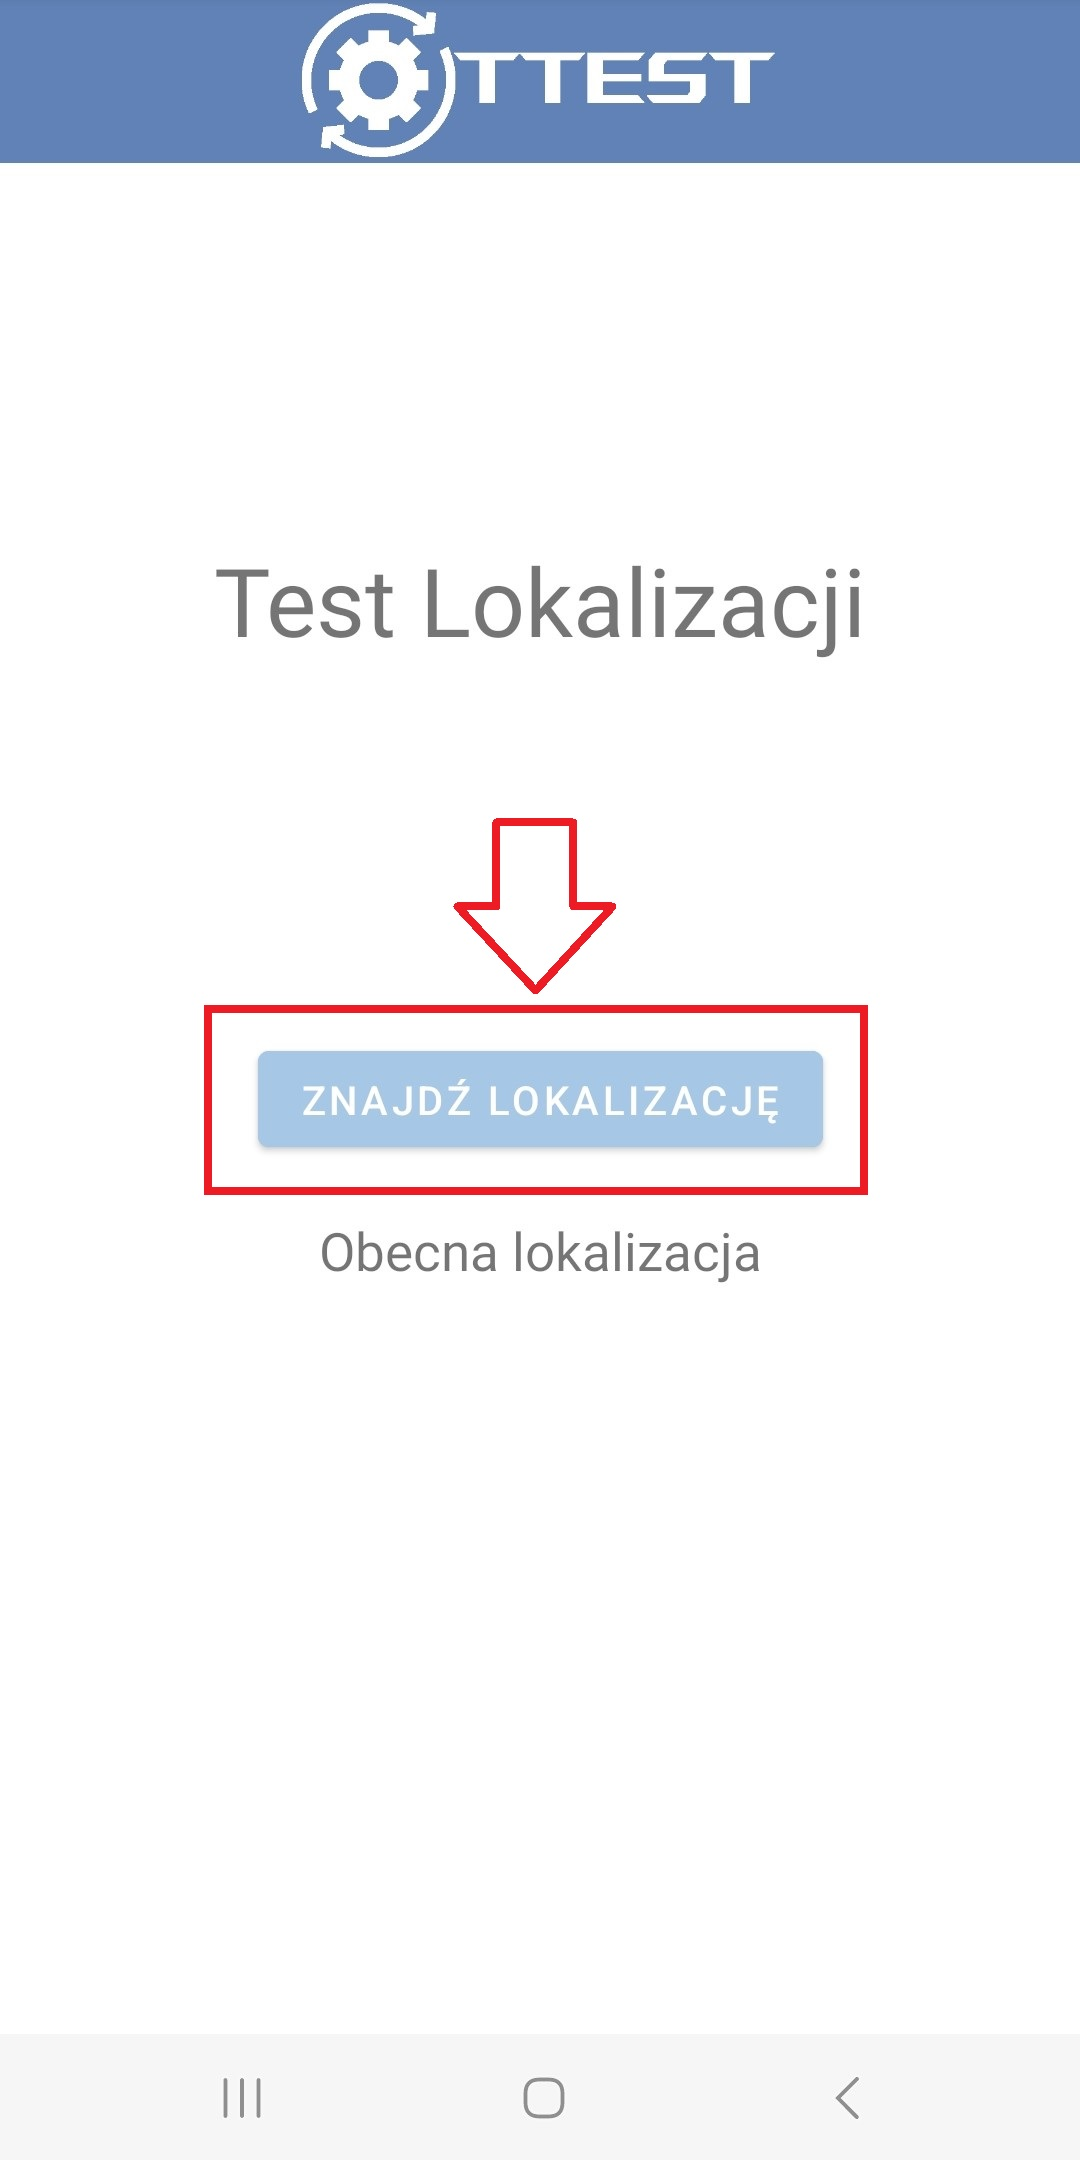
\includegraphics[angle=360, width=0.32\textwidth]{rys/punkt6/gps}
		\caption{Stona testowa GPS'a}
		\label{rys:gps}
	\end{center}
\end{figure}

Rysunek \ref{rys:gps1} przedstawia zrzuty ekranu potwierdzające pomyślny przebieg testu.

\begin{figure}[!hbt]
	\begin{center}
		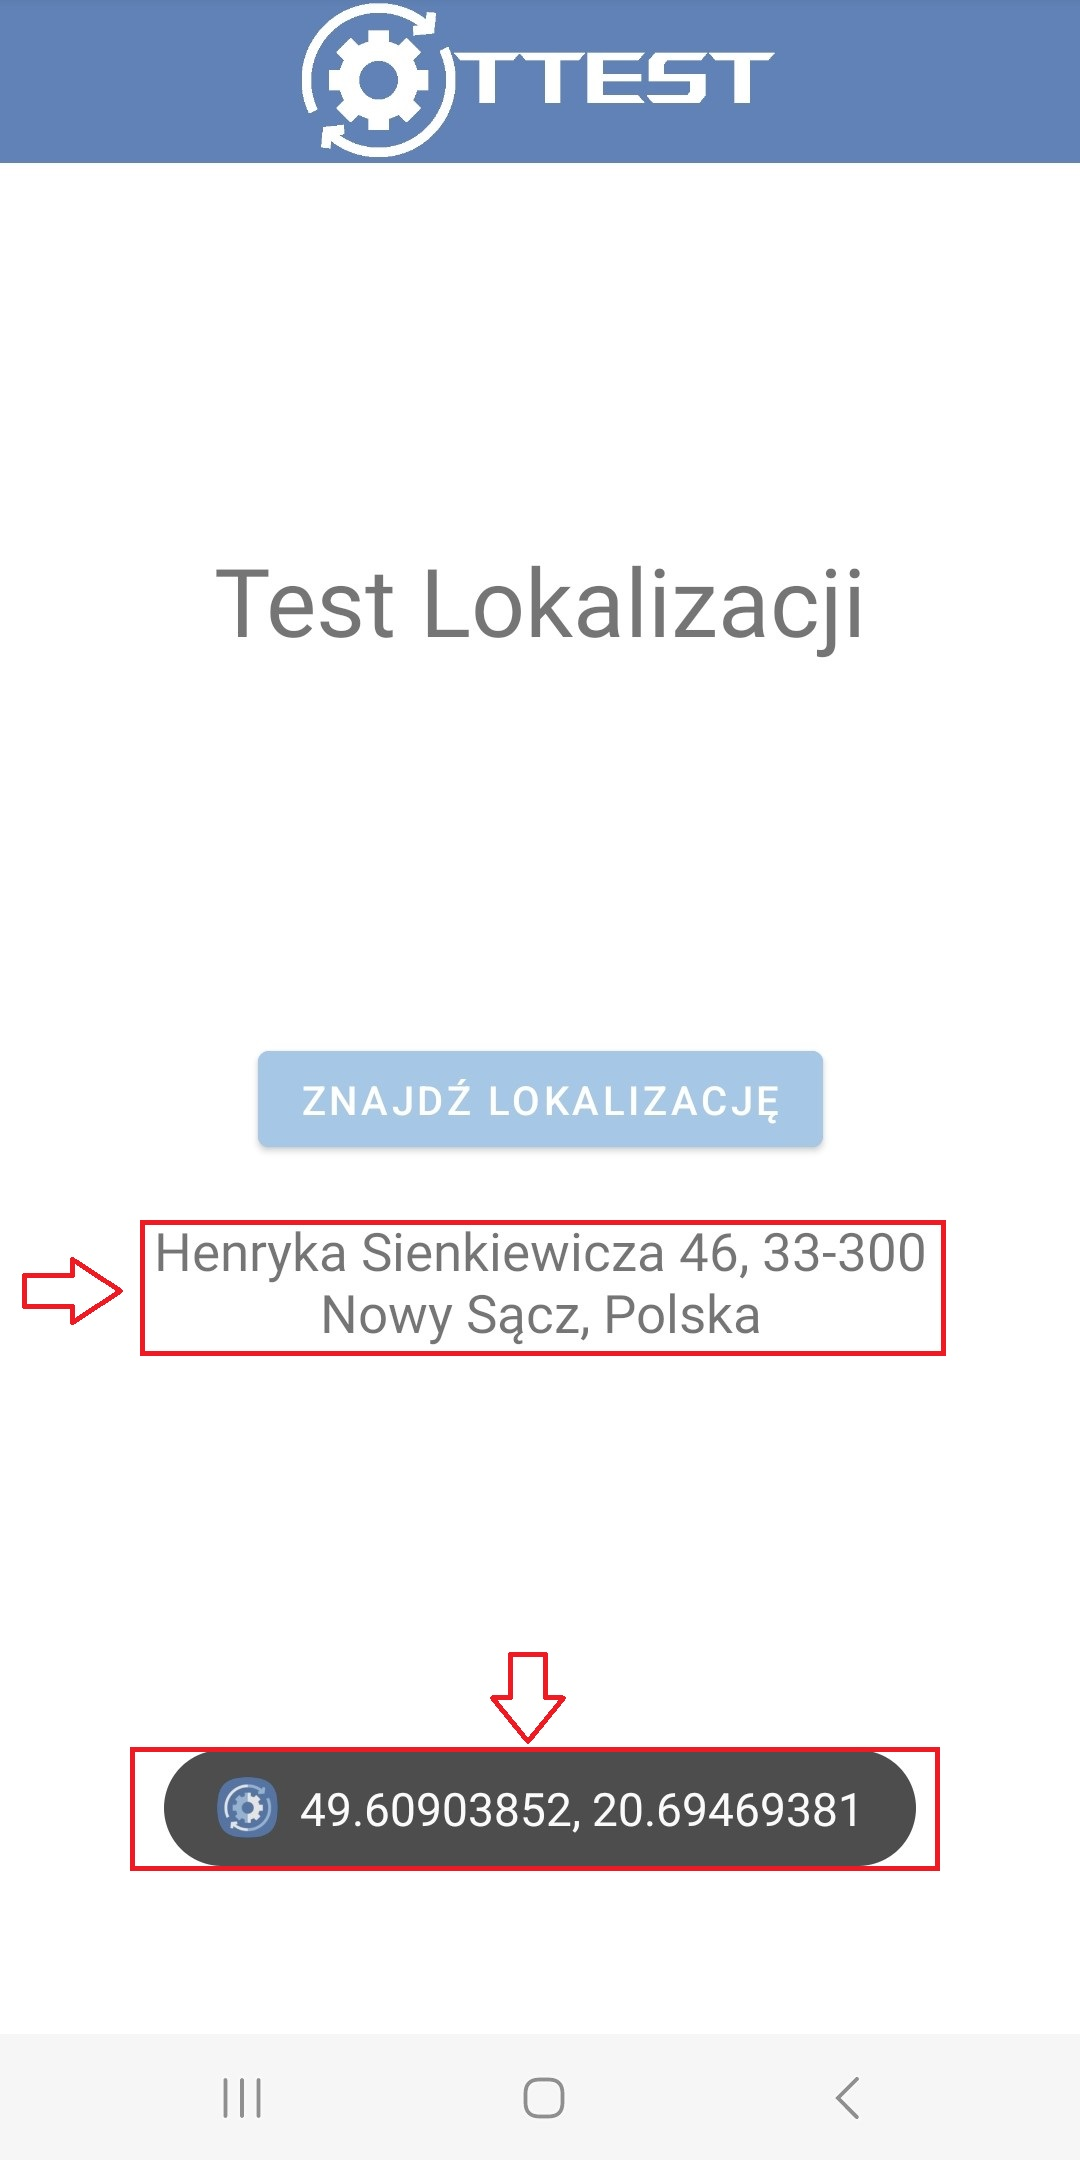
\includegraphics[angle=360, width=0.32\textwidth]{rys/punkt6/gps1}
		\caption{Działanie GPS'a}
		\label{rys:gps1}
	\end{center}
\end{figure}

\newpage


\subsection{Test Wifi}

\hspace{0.60cm}Aby uruchomić test wifi, w menu głównego wybieramy i klikamy na ikonkę, która znajduję się tuż pod testem czujnika zbliżeniowego. Rysunek \ref{rys:wifi} ukazuję miejsce które należy wybrać aby przejść do testu wifi. 

\begin{figure}[!hbt]
	\begin{center}
		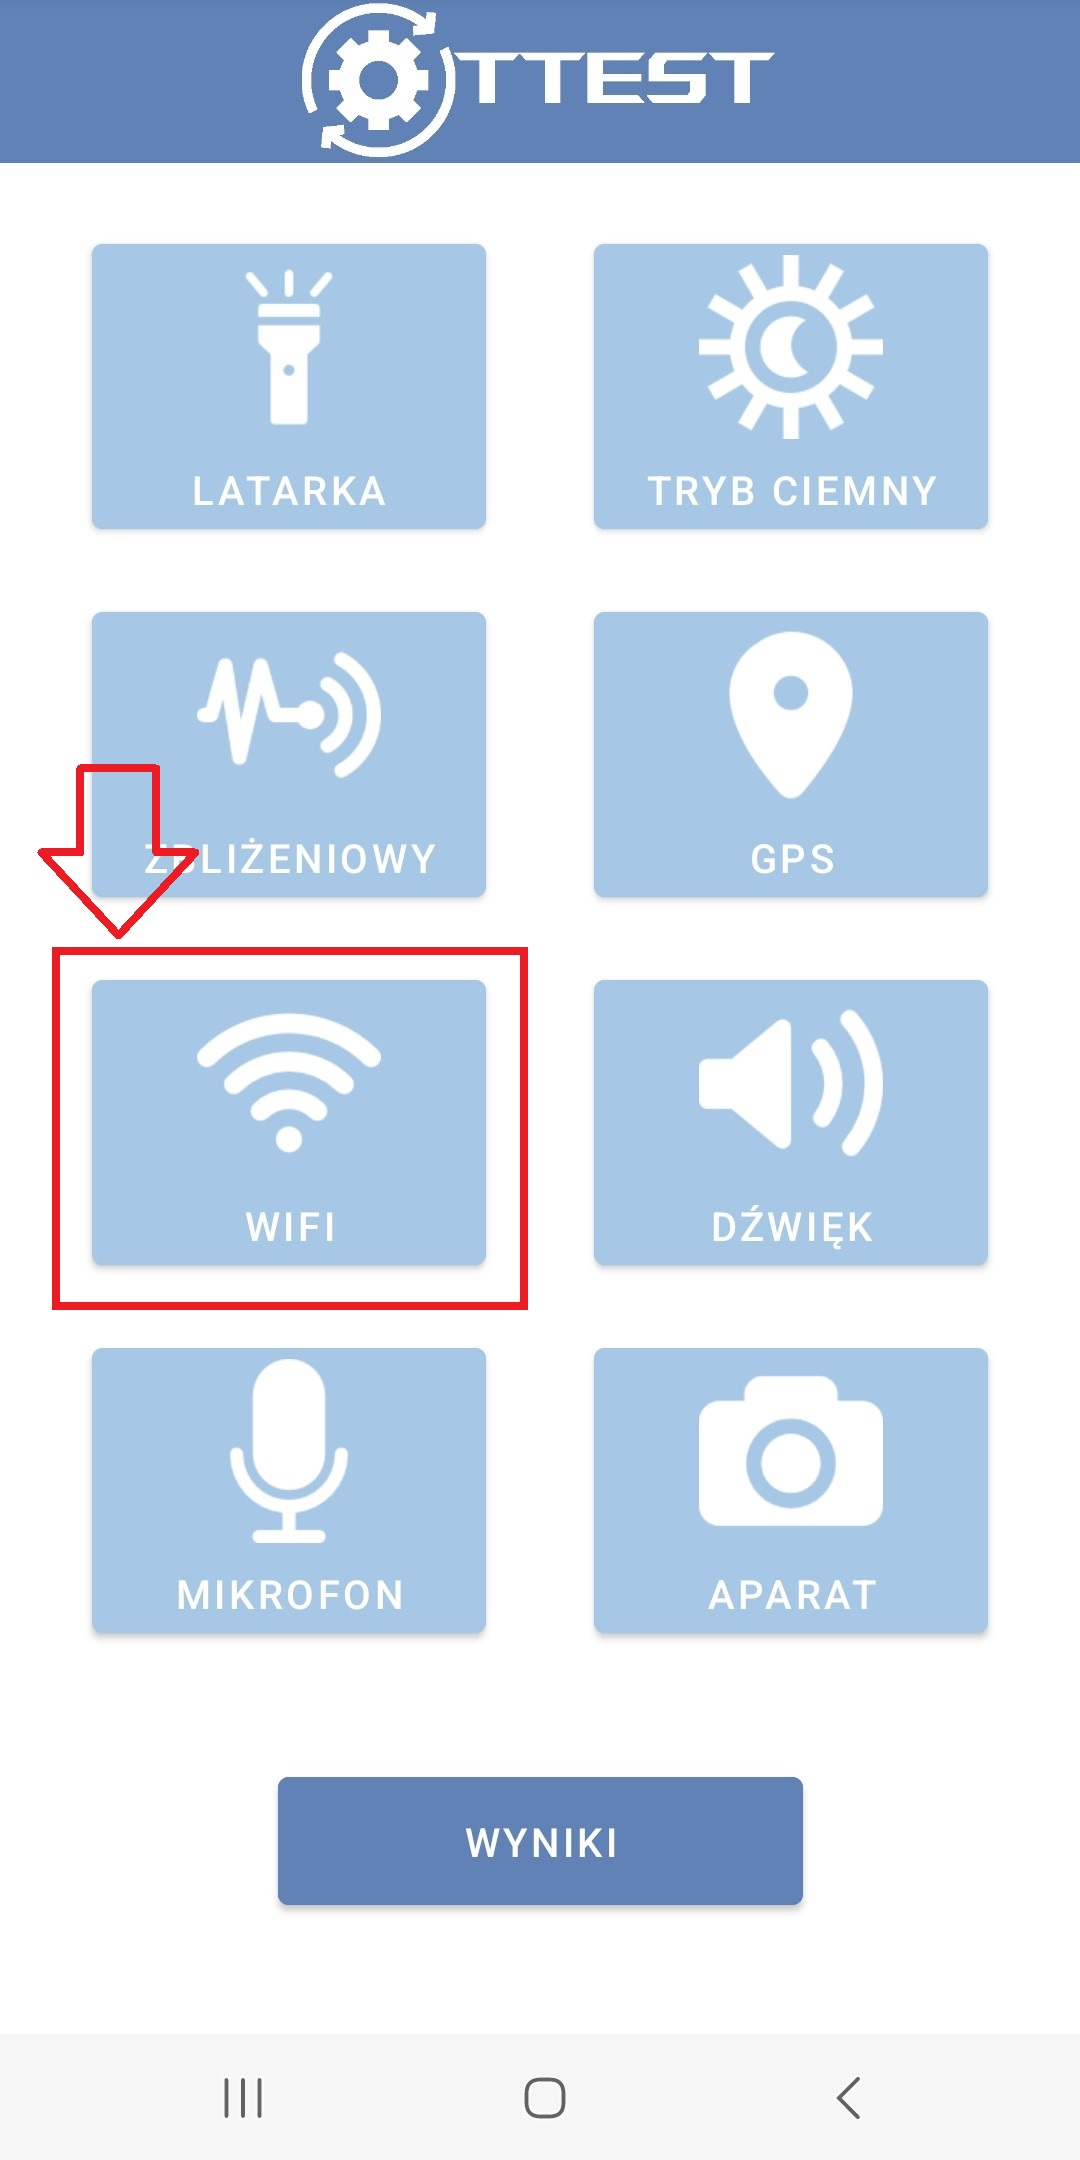
\includegraphics[angle=360, width=0.45\textwidth]{rys/punkt6/wifi}
		\caption{Wybór wifi}
		\label{rys:wifi}
	\end{center}
\end{figure}

\newpage 


Po przejściu do strony z testem wifi otrzymujemy informację aby uruchomić wifi na naszym telefonie i połączyć się z dostępną siecią. W innym przypadku nie będzie możliwe wykonanie testu oraz nie otrzymamy informacji o sieci. Rysunek \ref{rys:wifi1} prezentuje stronę z testem wifi.

\begin{figure}[!hbt]
	\begin{center}
		
\includegraphics[angle=360, width=0.45\textwidth]{rys/punkt6/wifi1}
		\caption{Strona testowa wifi}
		\label{rys:wifi1}
	\end{center}
\end{figure}

\newpage


Po połączeniu się z siecią za pomocą wifi, otrzymujemy komunikat który mówi, że aktualnie jesteśmy połączeni z siecią i możemy pobrać dostępne informację o niej. Aby otrzymać informacje o sieci należy kliknąć na przycisk znajdujący się na środku "Informacje o sieci". Rysunek \ref{rys:wifi2} prezentuje stronę z testem wifi po podłączeniu się do sieci.

\begin{figure}[!hbt]
	\begin{center}
		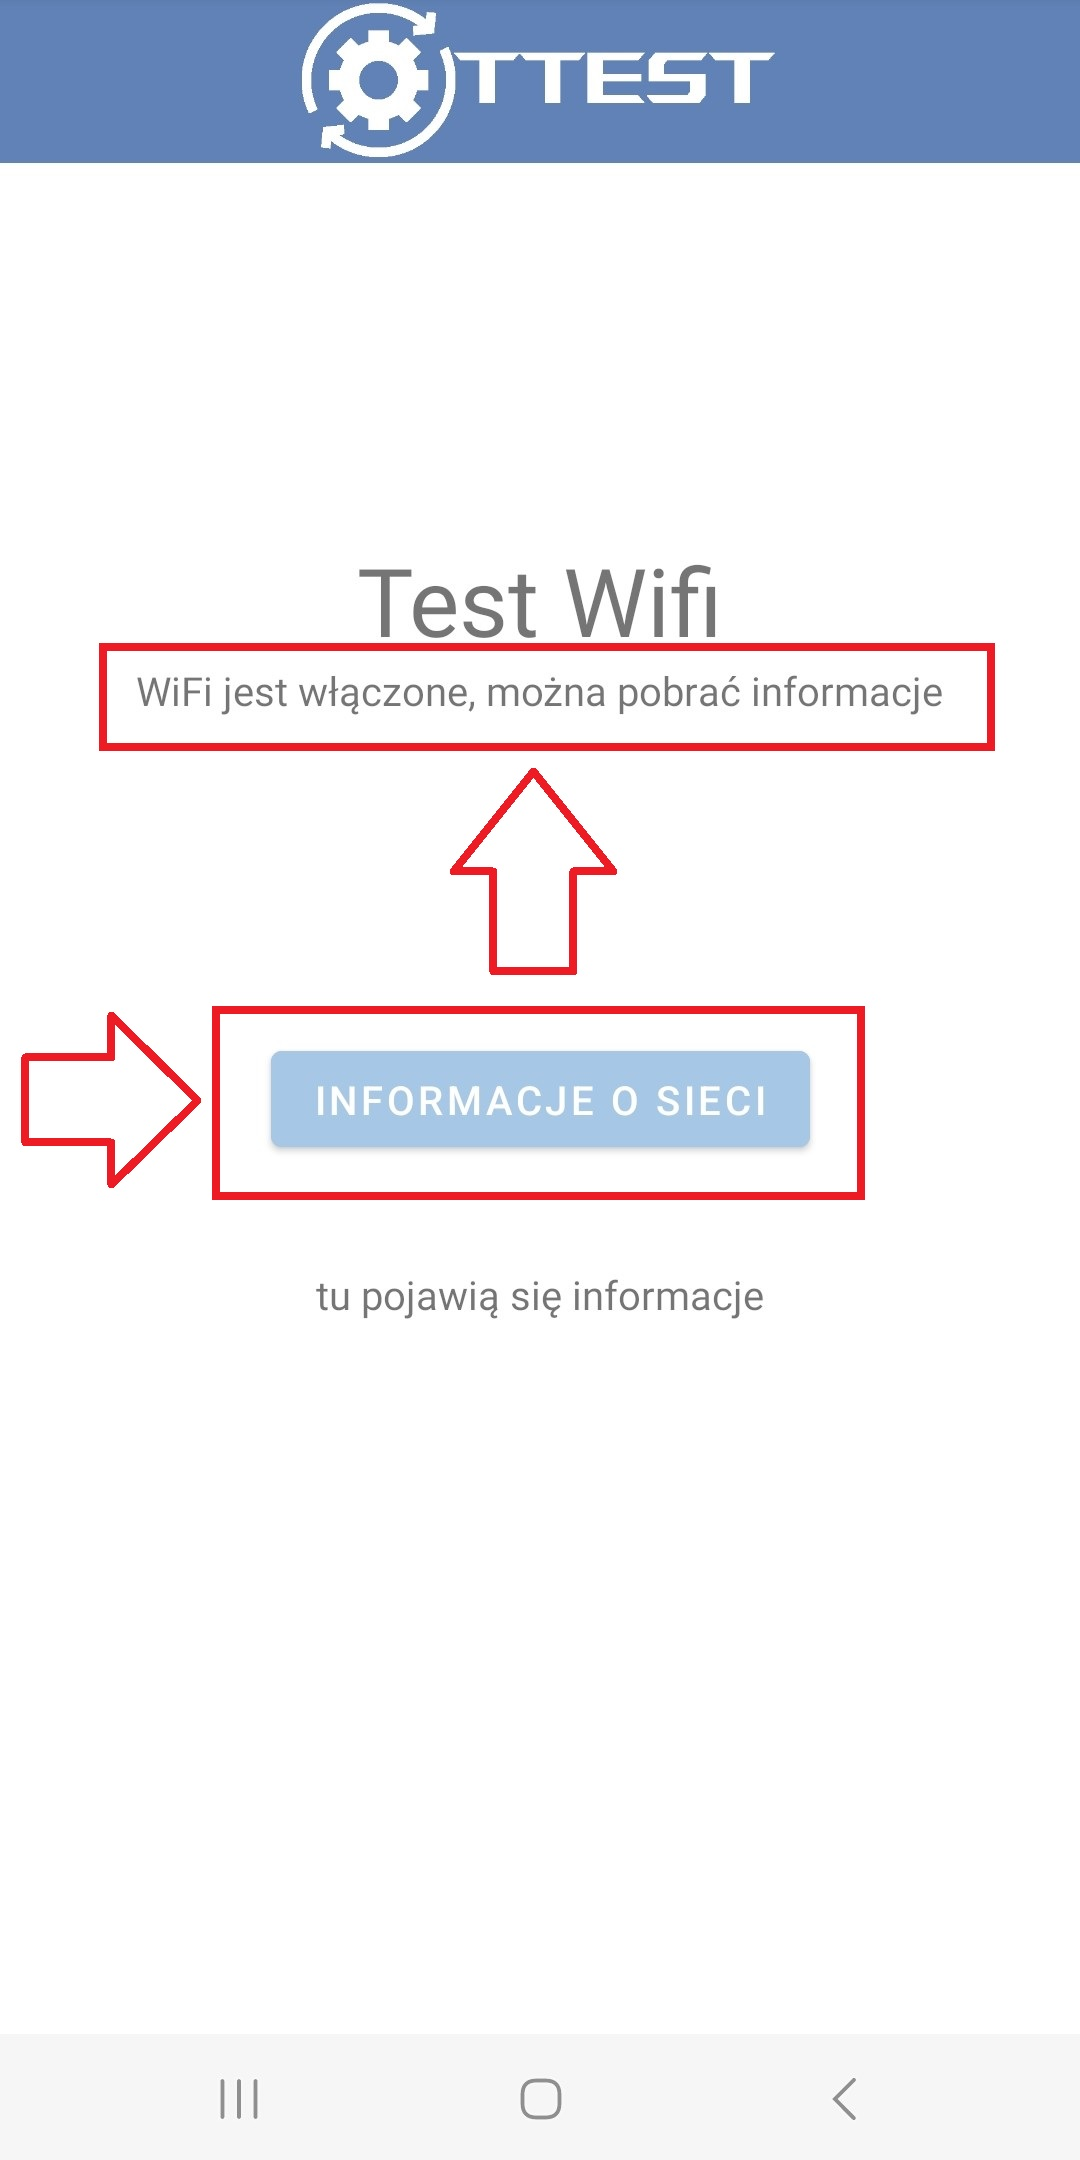
\includegraphics[angle=360, width=0.45\textwidth]{rys/punkt6/wifi2}
		\caption{Test wifi}
		\label{rys:wifi2}
	\end{center}
\end{figure}

\newpage


Po naciśnięciu na przycisk "Informacje o sieci" pojawią nam się wszystkie dostępne informacje o naszej sieci między innymi: Adres IP, Adres MAC Routera, SSID sieci do której jestesteśmy podłączeni oraz Wskaźnik mocy. Obrazek \ref{rys:wifi3} przedstawia zrzut ekranu potwierdzający pomyślny przebieg testu.

\begin{figure}[!hbt]
	\begin{center}
		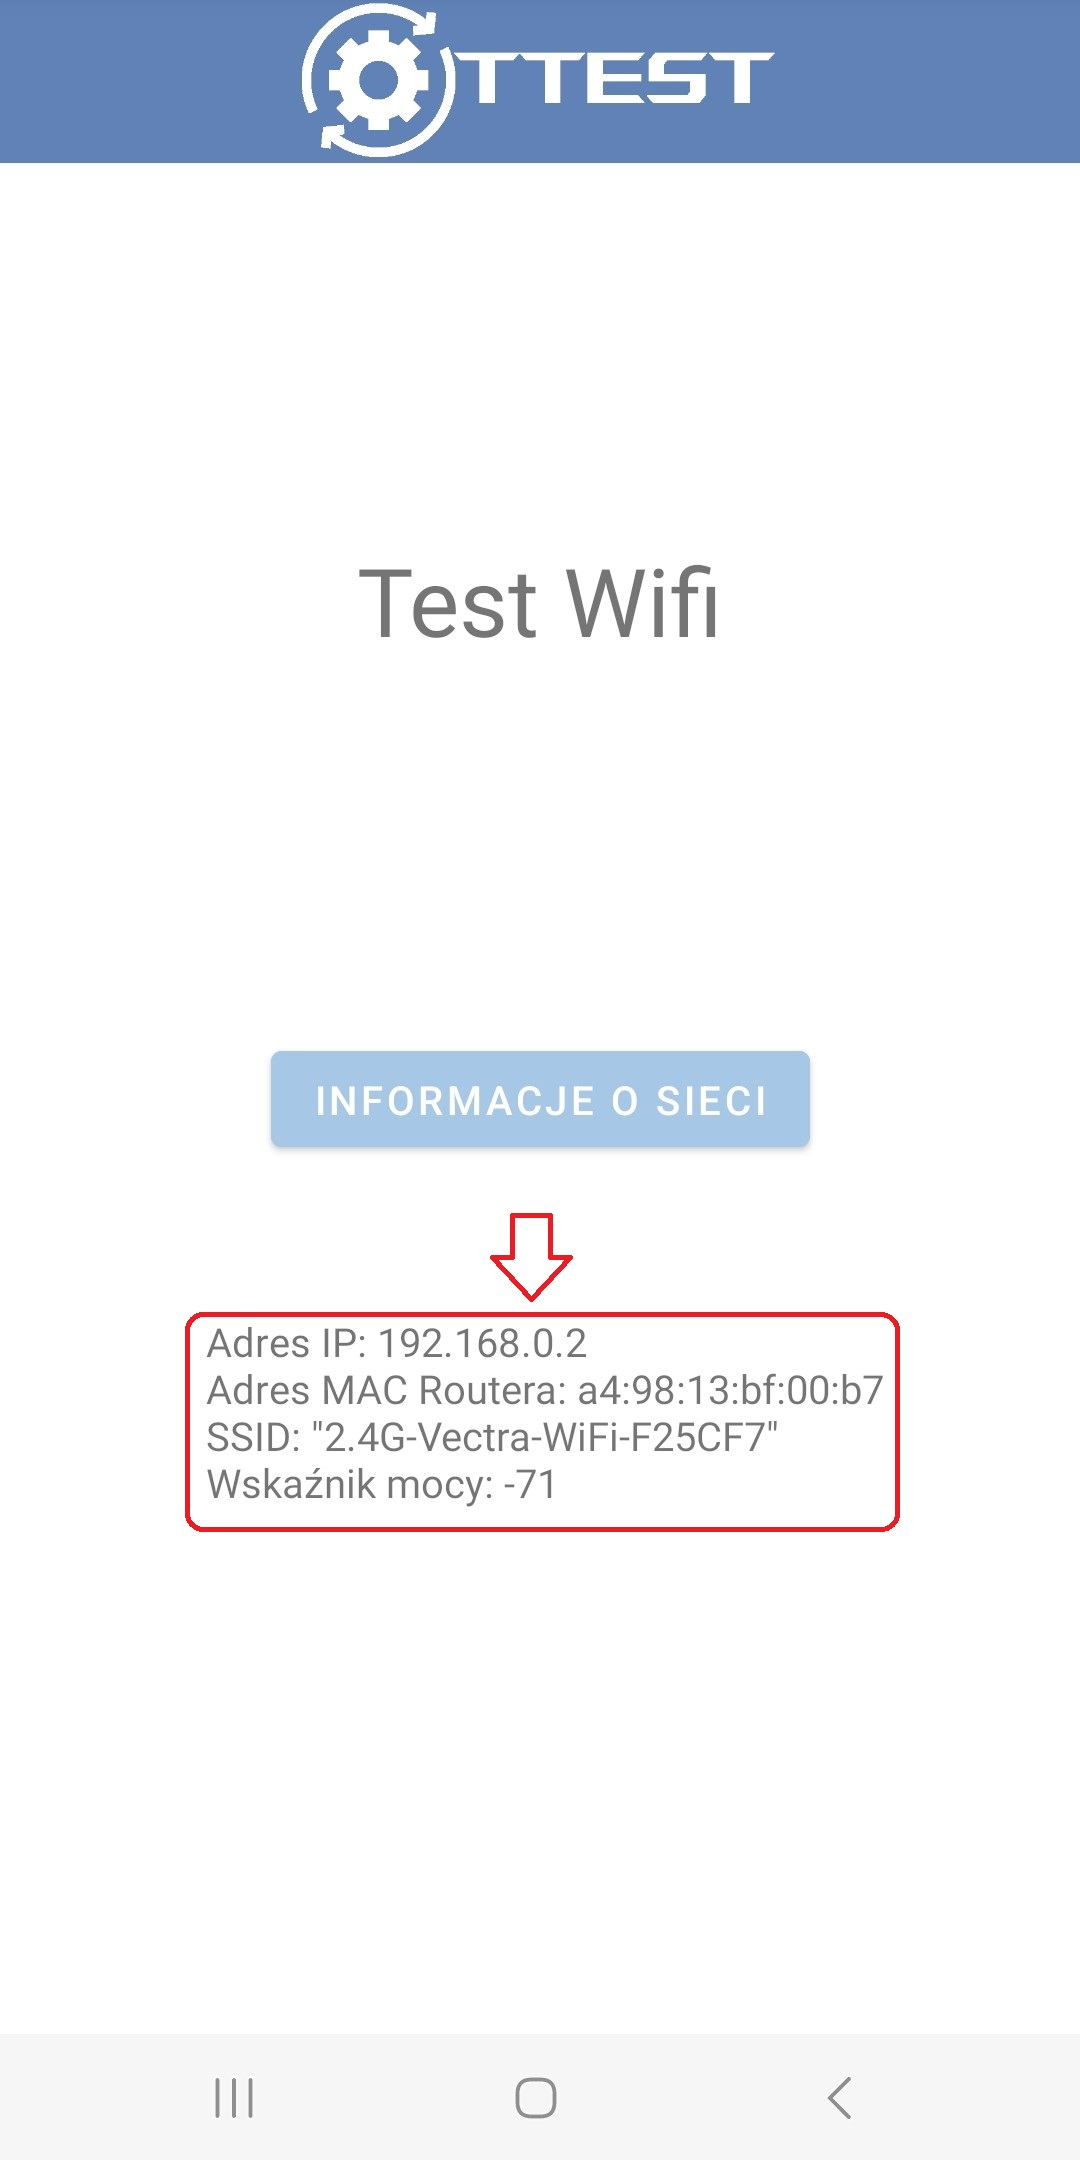
\includegraphics[angle=360, width=0.45\textwidth]{rys/punkt6/wifi3}
		\caption{Działanie wifi}
		\label{rys:wifi3}
	\end{center}
\end{figure}

\newpage


\subsection{Test dźwięku}

\hspace{0.60cm}Aby przejść do testu dźwięku należy kliknąć przycisk znajdujący się po prawej stronie tuż pod testem GPS'a. Rysunek \ref{rys:menu5} przedstawia miejsce które należy wybrać aby przejść do testu dźwięku.

\begin{figure}[!hbt]
	\begin{center}
		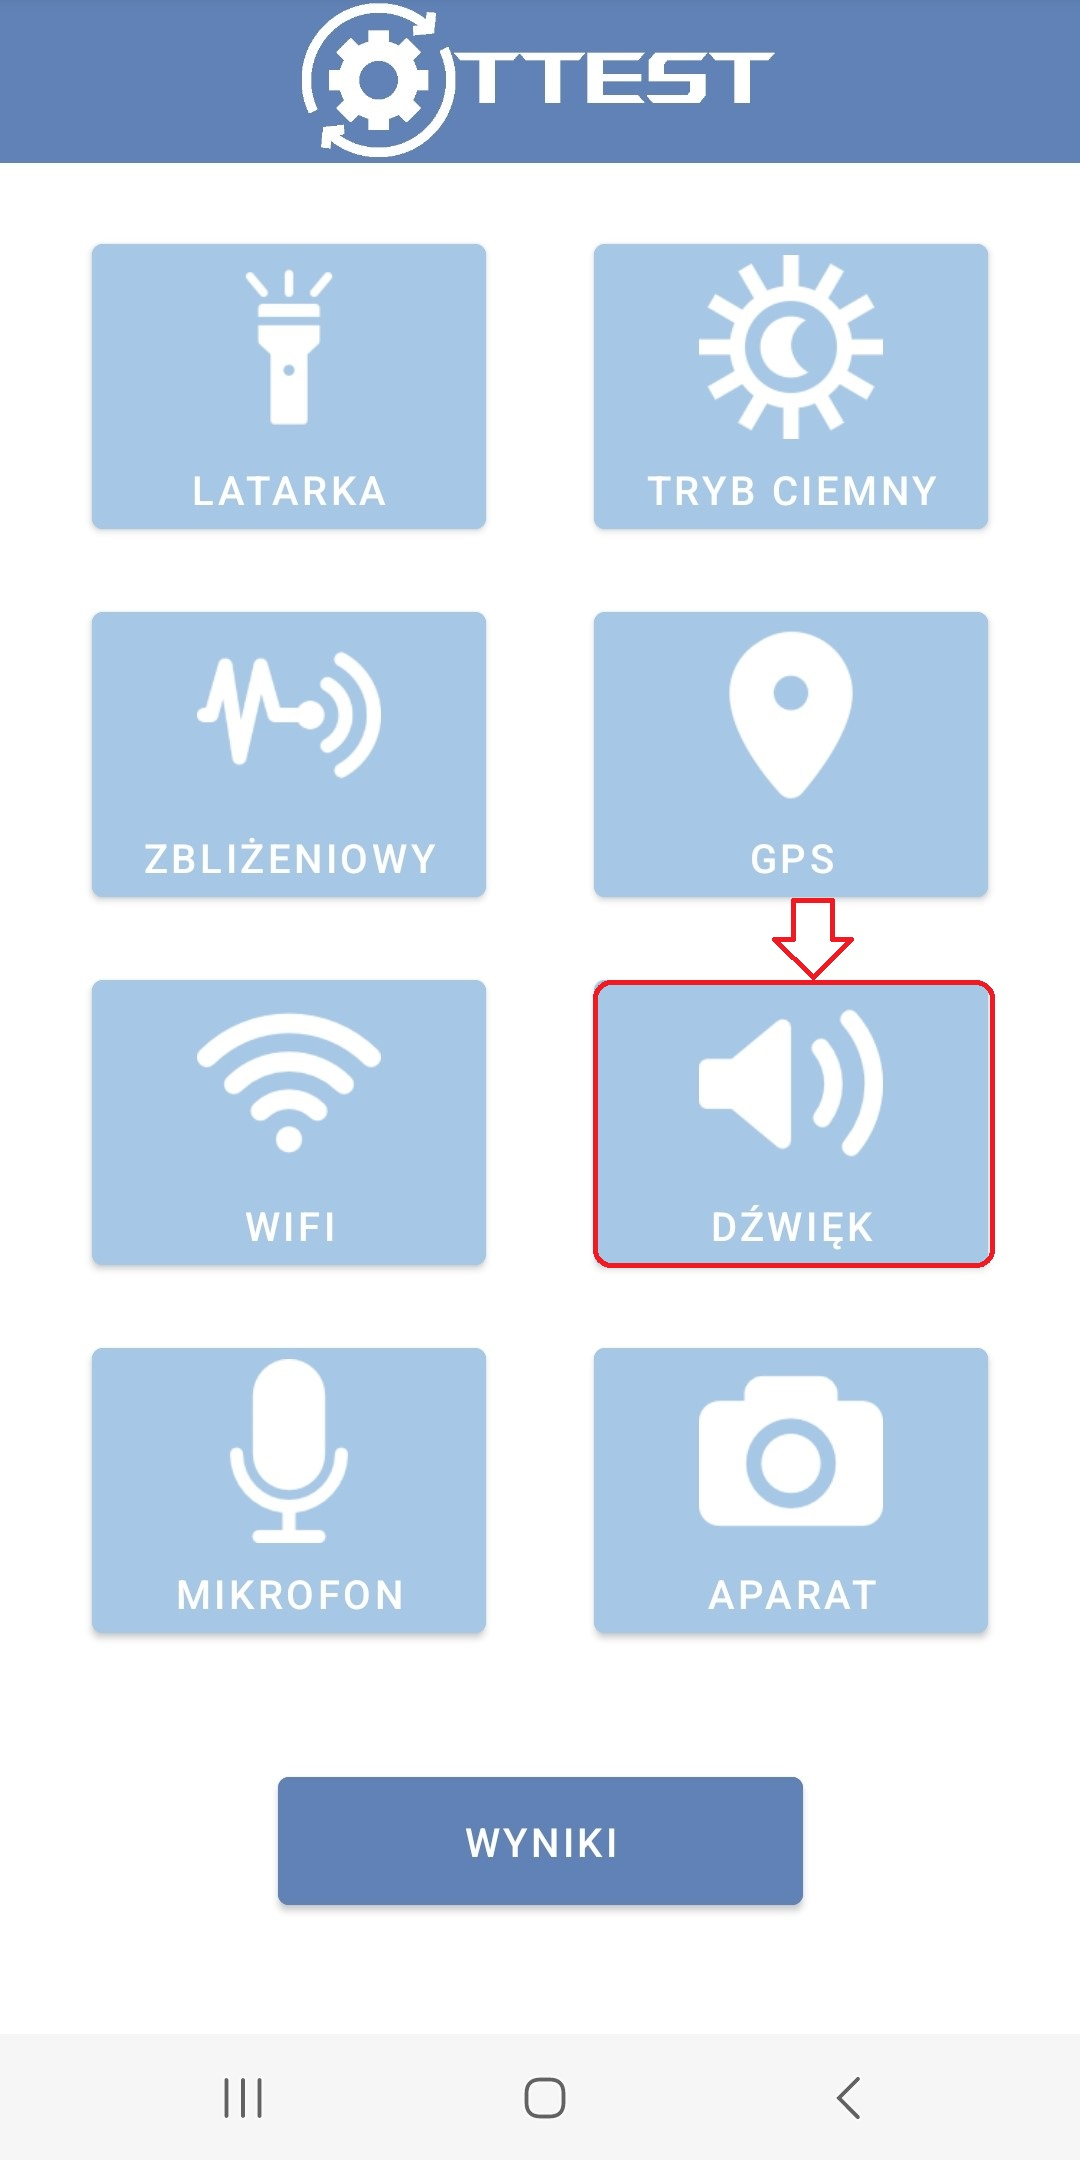
\includegraphics[angle=360, width=0.45\textwidth]{rys/punkt6/menu5}
		\caption{Wybór testu dźwięku}
		\label{rys:menu5}
	\end{center}
\end{figure}

Po przekierowaniu na stronę z testem dostrzegamy że na środku znajduję się przycisk z napisem - "Naciśnij". Rysunek \ref{rys:dźwięk} prezentuję przycisk uruchamiający test dźwięku.

Gdy naciśniemy przycisk z głośników telefonu usłyszymy dźwięk ćwierkających ptaków. Co więcej pod przyciskiem wyświetli nam się komunikat, który informuję nas o tym, że nagranie jest odtwarzane. 

\newpage

\begin{figure}[!hbt]
	\begin{center}
		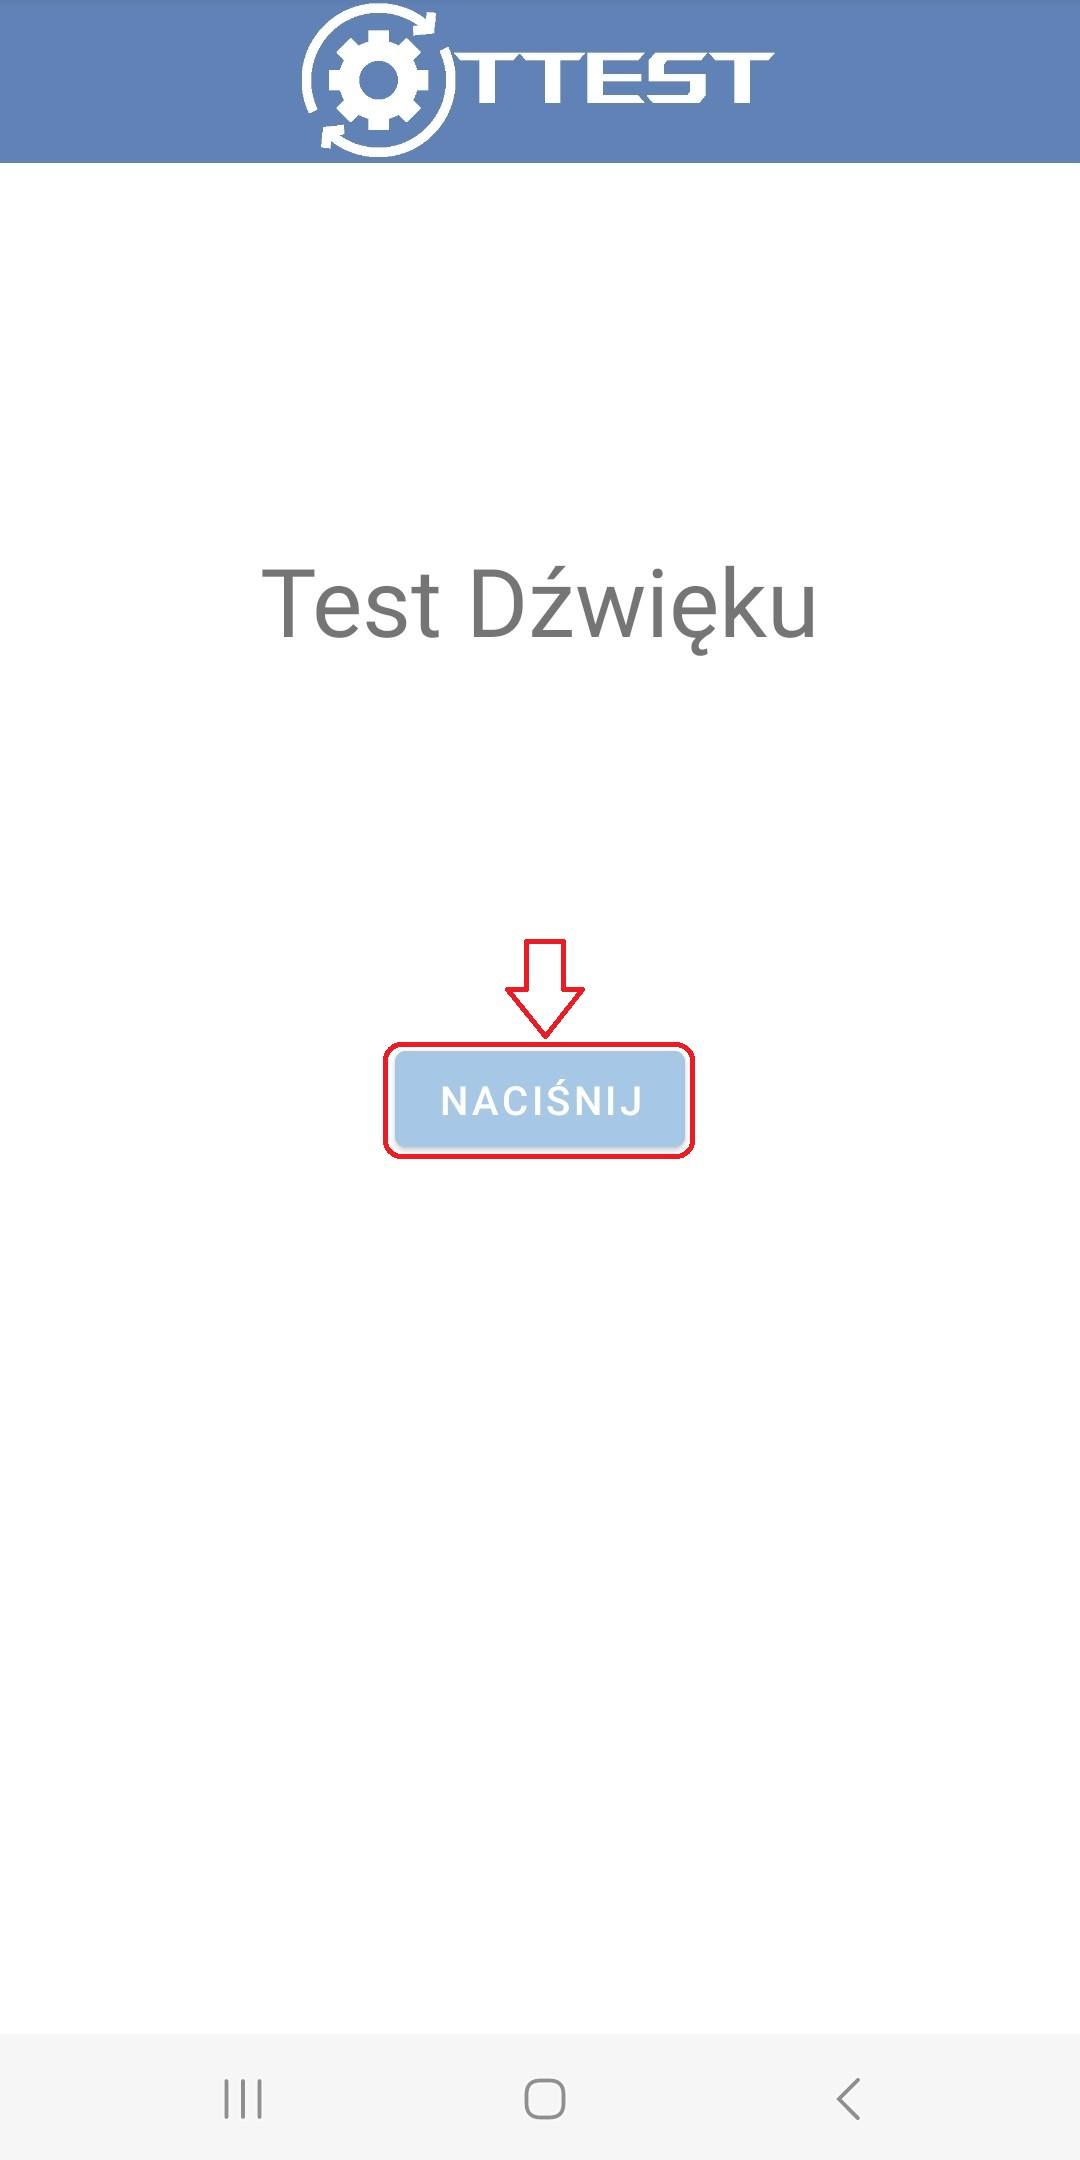
\includegraphics[angle=360, width=0.31\textwidth]{rys/punkt6/dźwięk}
		\caption{Strona testowa dźwięku}
		\label{rys:dźwięk}
	\end{center}
\end{figure}

Rysunek \ref{rys:dźwięk2} przedstawia zrzut ekranu potwierdzający pomyślny przebieg testu.

\begin{figure}[!hbt]
	\begin{center}
		
\includegraphics[angle=360, width=0.31\textwidth]{rys/punkt6/dźwięk2}
		\caption{Test dźwięku}
		\label{rys:dźwięk2}
	\end{center}
\end{figure}

\newpage


\subsection{Test mikrofonu}

\hspace{0.60cm}Aby przejść do testu mikrofonu należy kliknąć przycisk znajdujący się po lewej stronie tuż pod testem wifi. Rysunek \ref{rys:menu6} przedstawia miejsce które należy wybrać aby przejść do testu mikrofonu.

\begin{figure}[!hbt]
	\begin{center}
		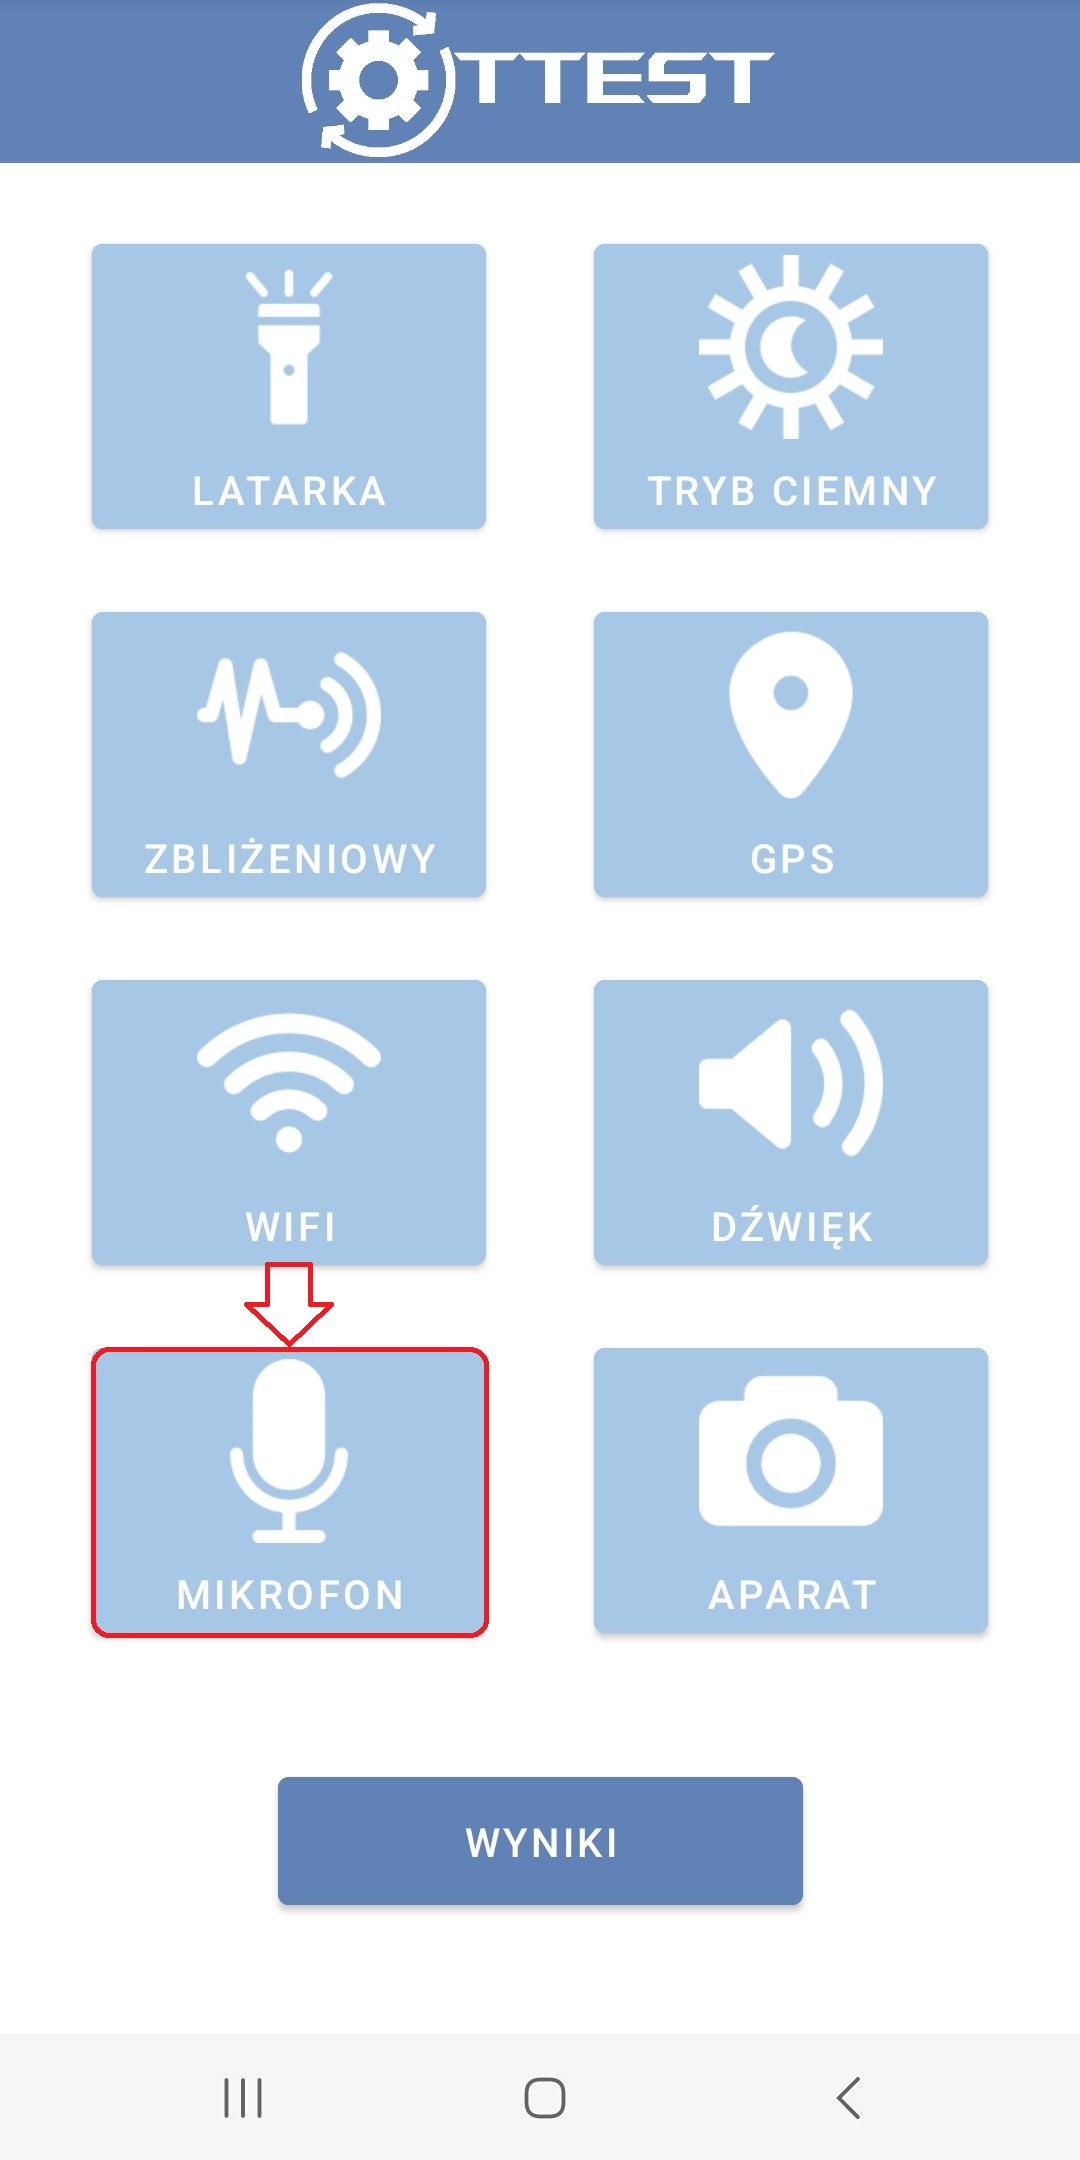
\includegraphics[angle=360, width=0.45\textwidth]{rys/punkt6/menu6}
		\caption{Wybór testu mikrofonu}
		\label{rys:menu6}
	\end{center}
\end{figure}

Po przekierowaniu na stronę z testem dostrzegamy że na środku znajduję się trzry przyciski kolejno: Start, Stop oraz Play. 

\newpage


Przycisk z napisem - "Start" rozpoczyna test oraz nagrywa wszystko to co mówimy. Ponadto u dołu ekranu pojawia się komunikat, który informuję nas o rozpoczęciu nagrywania. Rysunek \ref{rys:mikrofon1} prezentuję przycisk Startu w teście mikrofonu.

\begin{figure}[!hbt]
	\begin{center}
		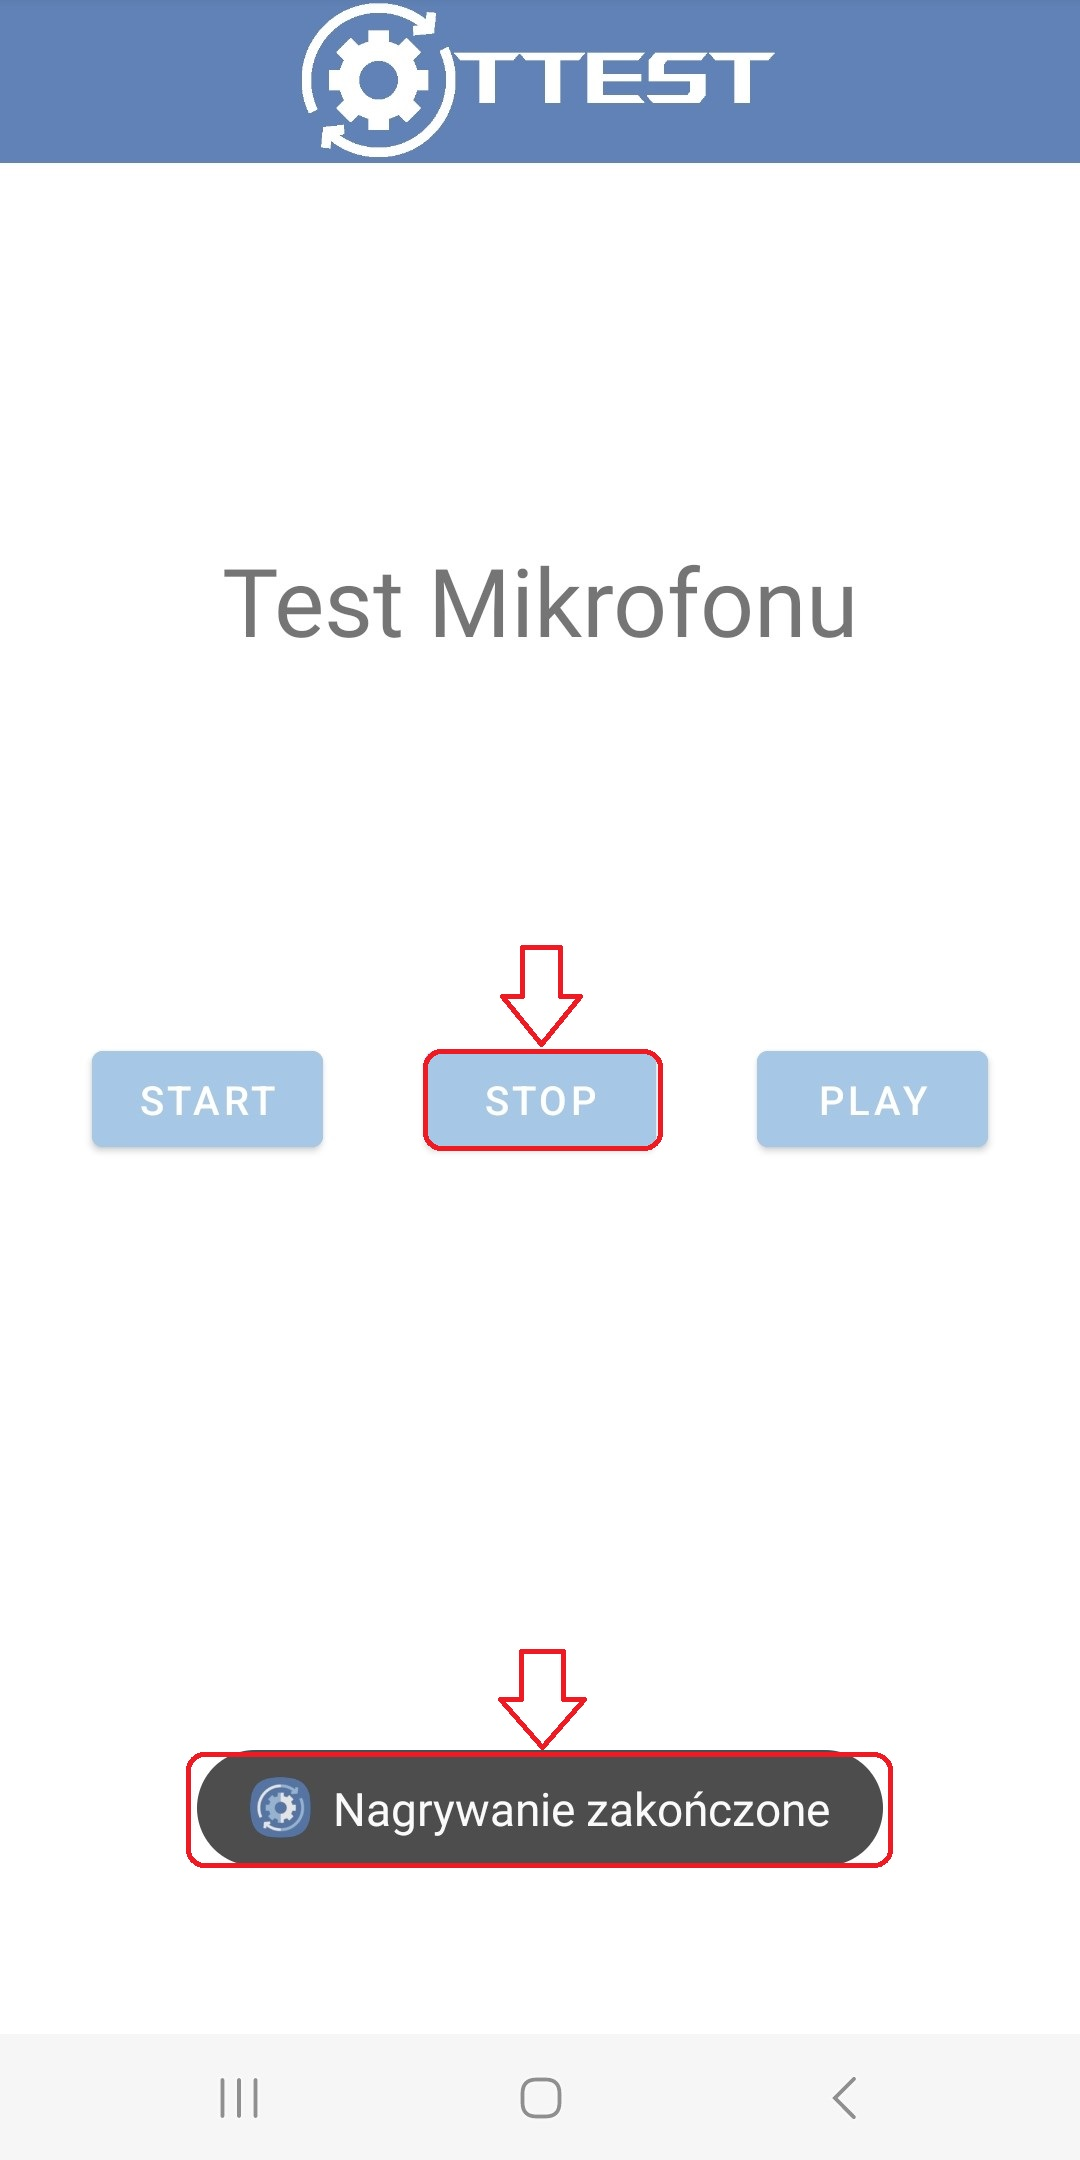
\includegraphics[angle=360, width=0.45\textwidth]{rys/punkt6/mikrofon1}
		\caption{Działanie przycisku Start - Mikrofon}
		\label{rys:mikrofon1}
	\end{center}
\end{figure}

\newpage


Aby zatrzymać nagrywanie wystarczy przycisnąć drugi przycisk - "Stop". Podobnie jak w przypadku przycisku "Start", u dołu ekranu pojawi się informacja o tym, że nagrywanie zostało zakończone. Rysunek \ref{rys:mikrofon2} prezentuję przycisk Stopu w teście mikrofonu.

\begin{figure}[!hbt]
	\begin{center}
		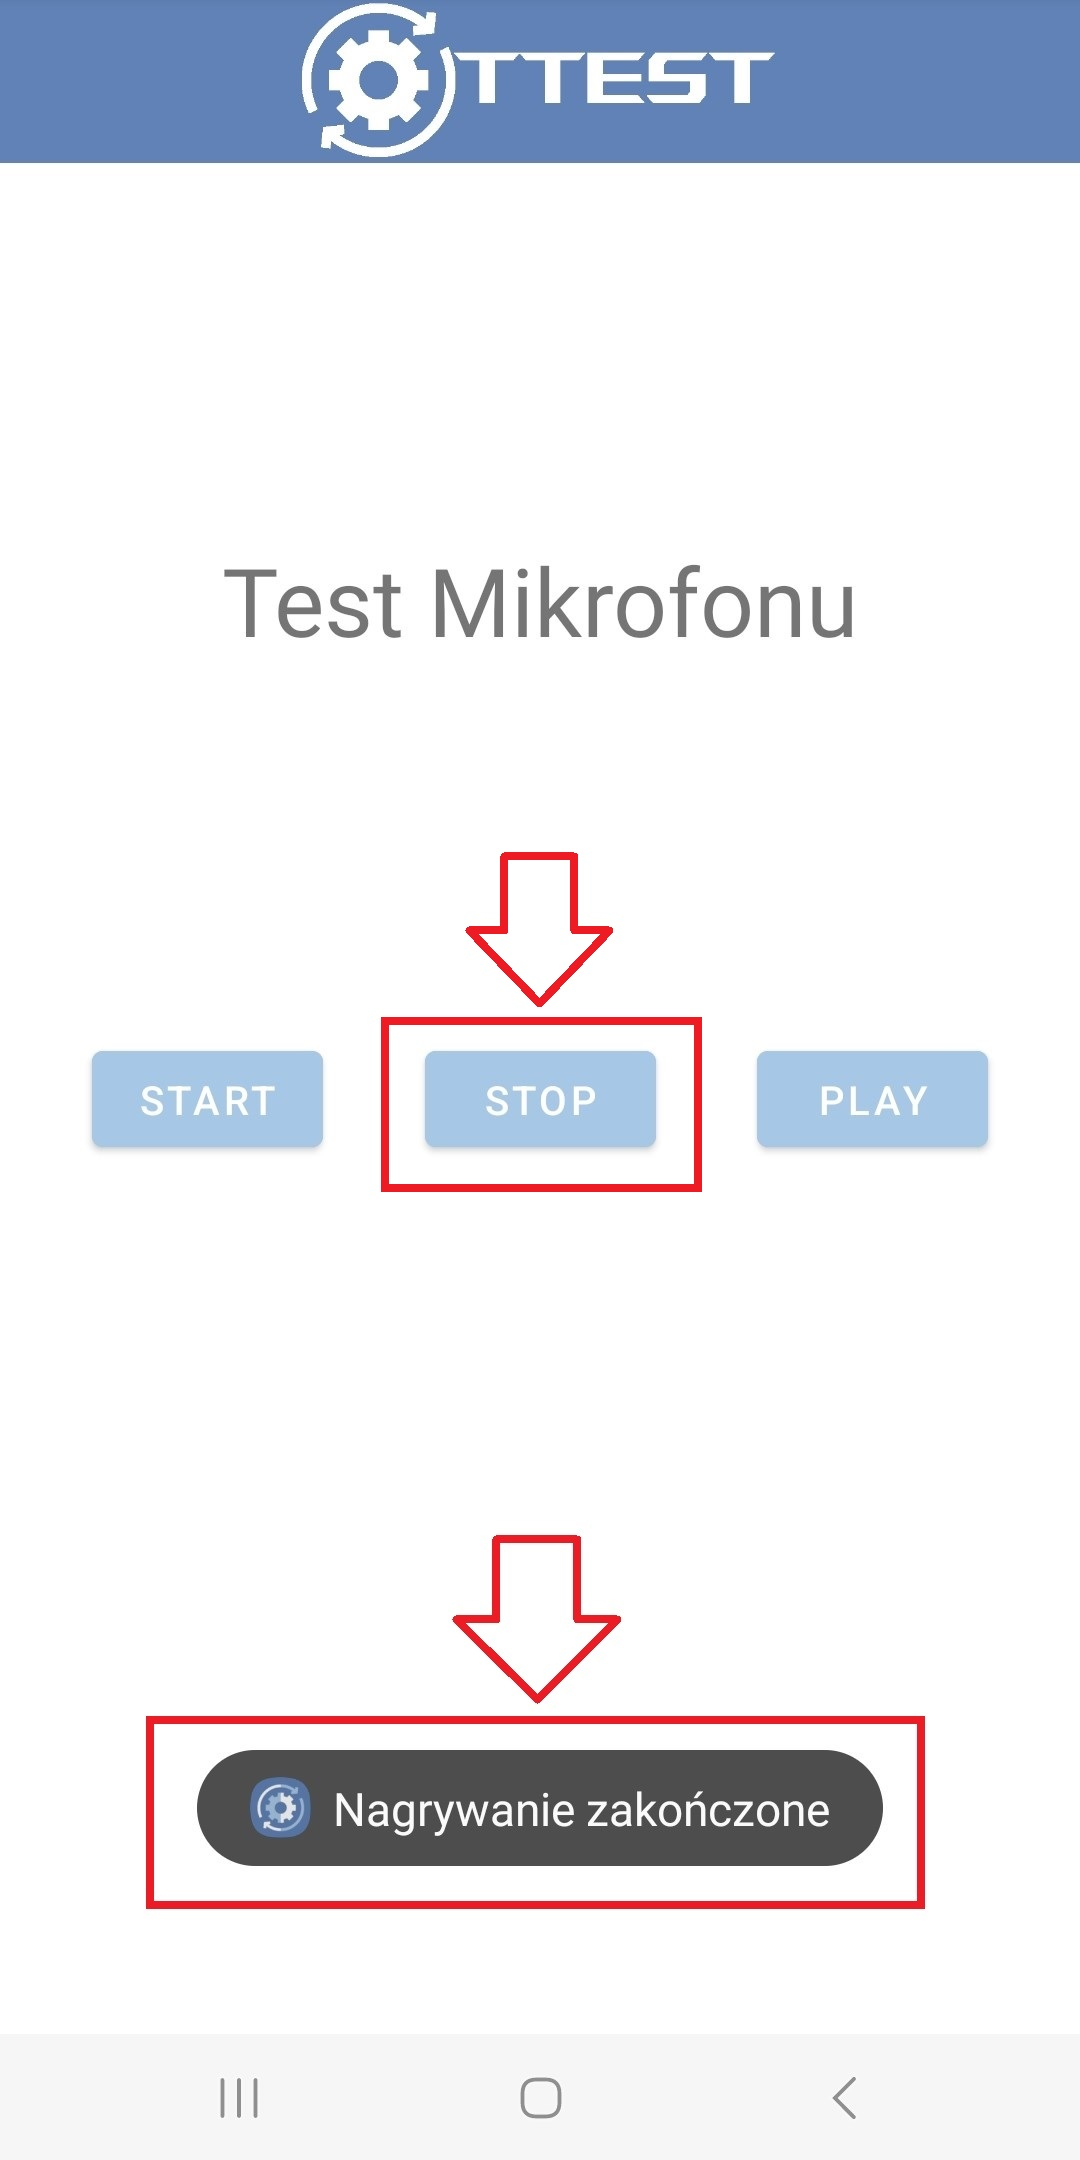
\includegraphics[angle=360, width=0.45\textwidth]{rys/punkt6/mikrofon2}
		\caption{Działanie przycisku Stop - Mikrofon}
		\label{rys:mikrofon2}
	\end{center}
\end{figure}

\newpage


Ostatni z przycisków - "Play" pozwala na odtworzenie nagranego wcześniej nagrania. Pod przyciskami zarówno jak przy przycisku Start jak i Stop, pojawia się informacja o tym, że nagranie jest odtwarzane. Rysunek \ref{rys:mikrofon3} prezentuję przycisk Play w teście mikrofonu.

\begin{figure}[!hbt]
	\begin{center}
		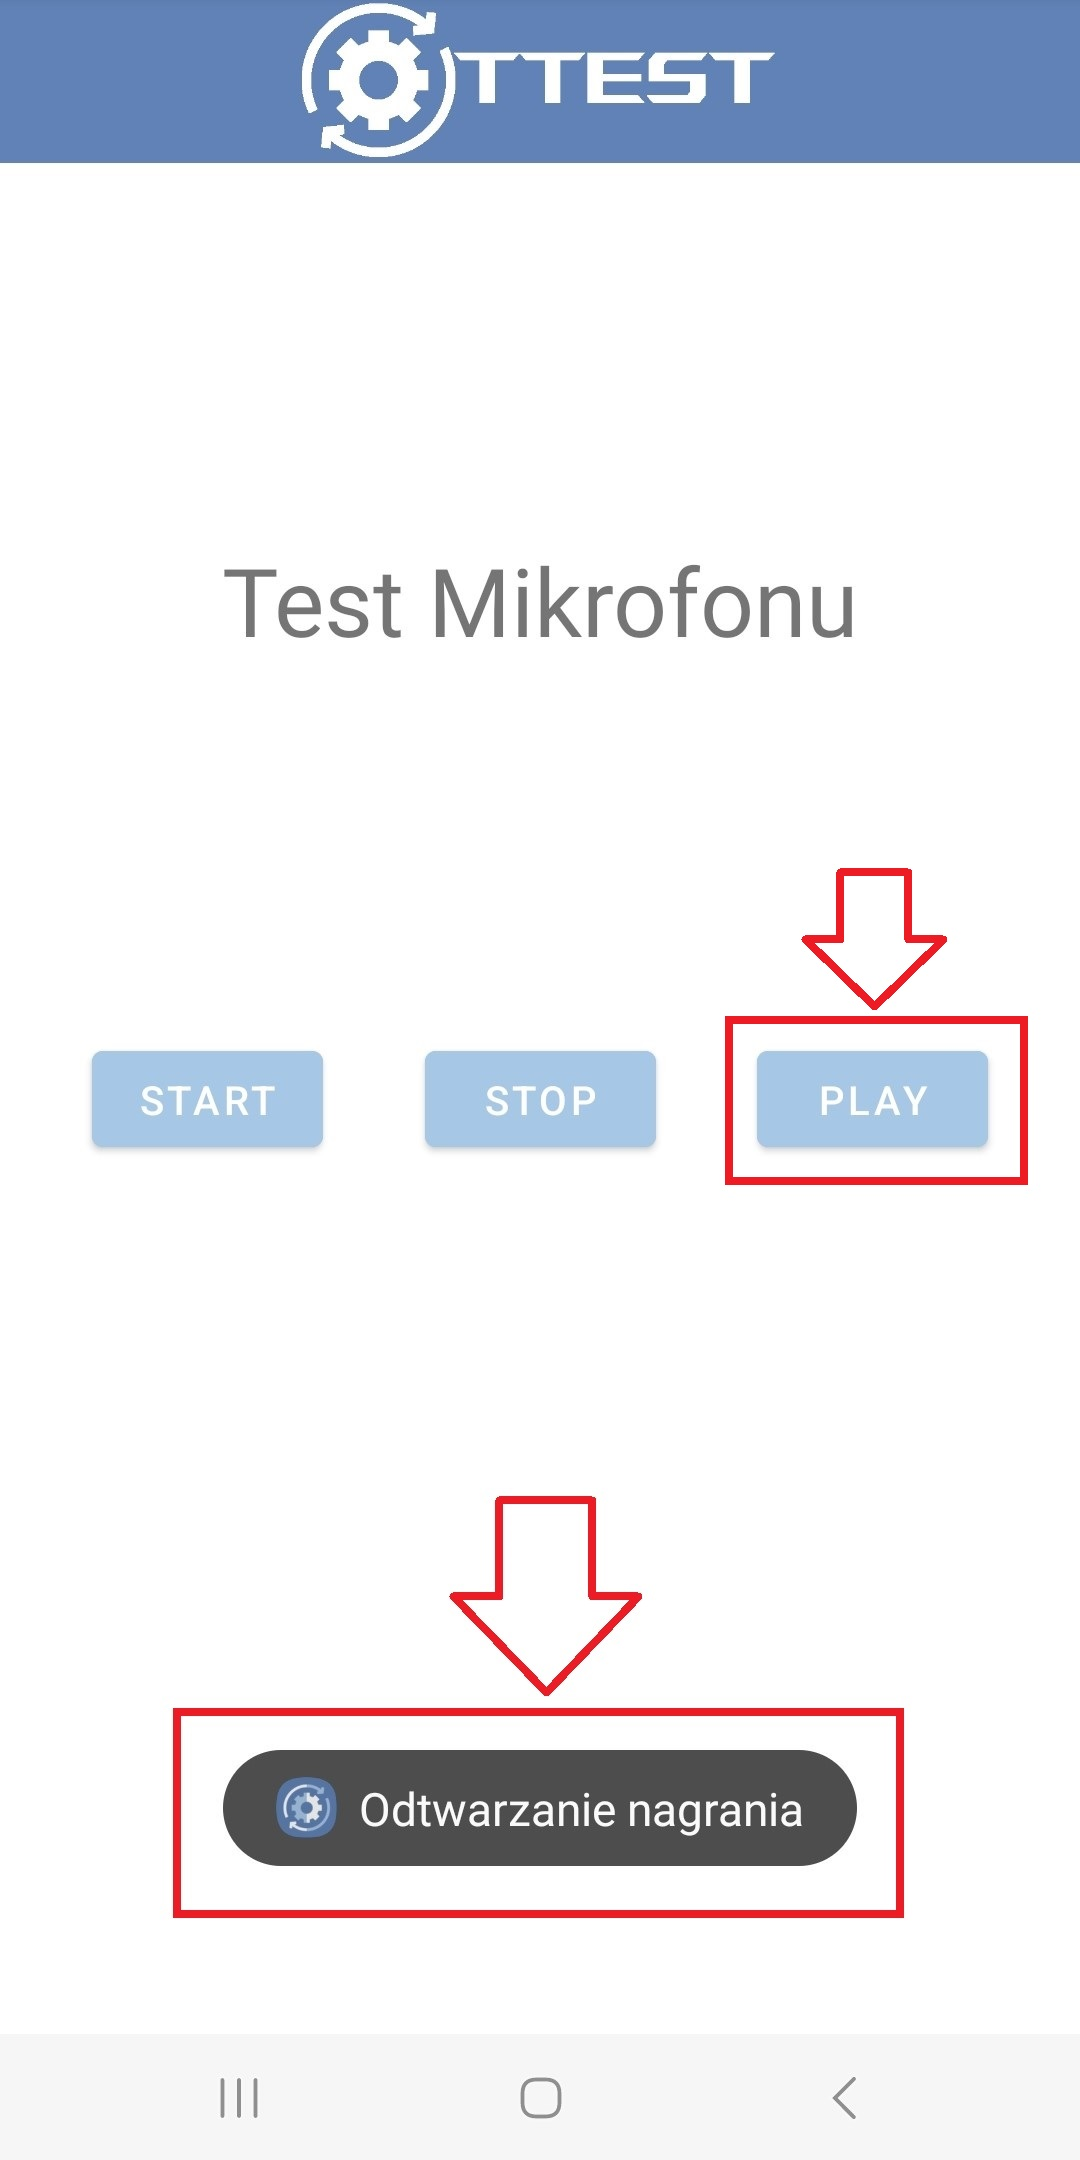
\includegraphics[angle=360, width=0.45\textwidth]{rys/punkt6/mikrofon3}
		\caption{Działanie przycisku Play - Mikrofon}
		\label{rys:mikrofon3}
	\end{center}
\end{figure}

\newpage


\subsection{Test aparatu}

\hspace{0.60cm}Aby przejść do testu aparatu należy w menu głównym wybrać i kliknąć przycisk znajdujący się po prawej stronie tuż pod testem dźwięku. Rysunek \ref{rys:menu7} przedstawia miejsce które należy wybrać aby przejść do testu aparatu.

\begin{figure}[!hbt]
	\begin{center}
		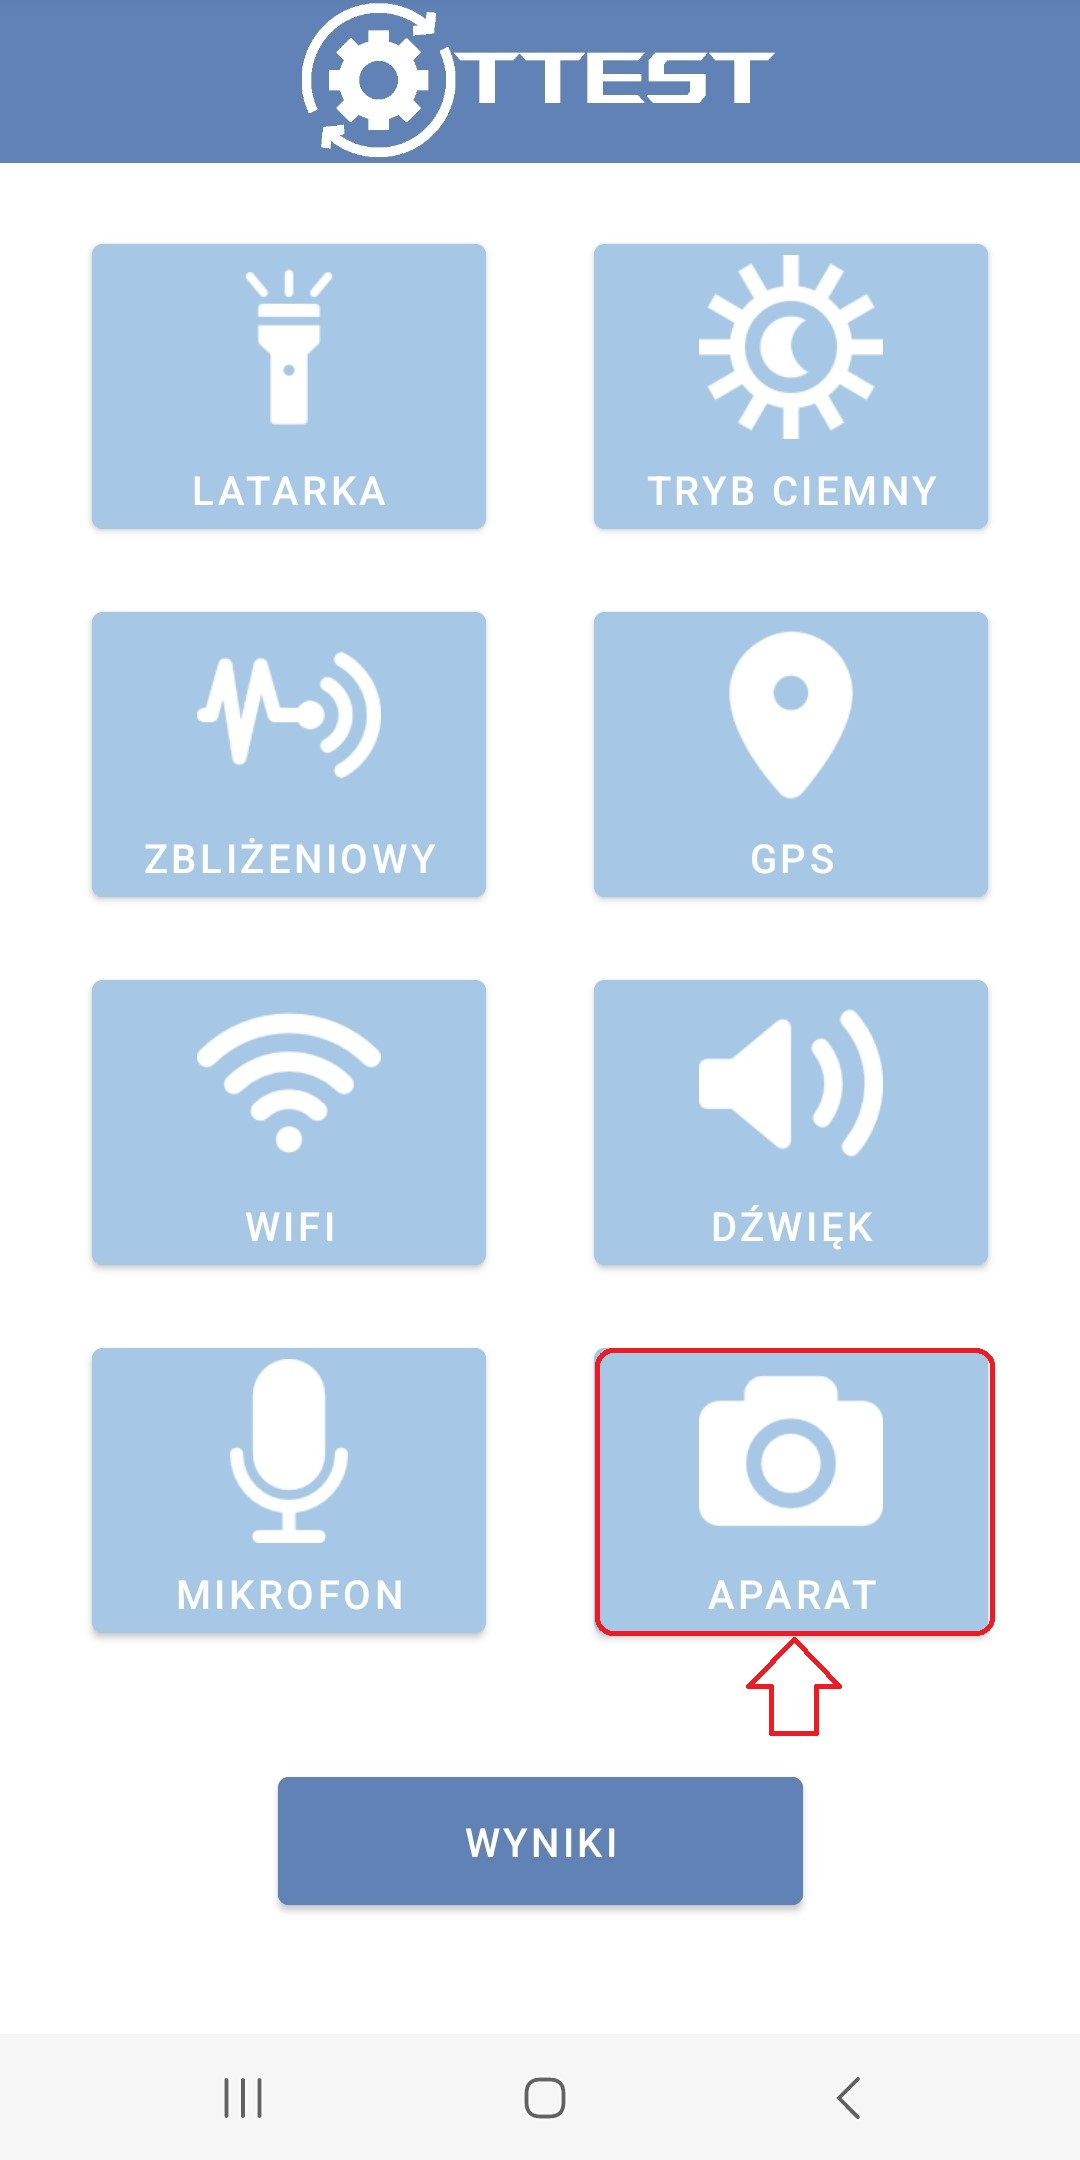
\includegraphics[angle=360, width=0.45\textwidth]{rys/punkt6/menu7}
		\caption{Wybór testu aparatu}
		\label{rys:menu7}
	\end{center}
\end{figure}

\newpage


Po przejściu na stronę z testem dostrzegamy że na środku znajduję się przycisk z napisem - "Zrób zdjęcie". Rysunek \ref{rys:aparat} prezentuję przycisk uruchamiający test aparatu.

\begin{figure}[!hbt]
	\begin{center}
		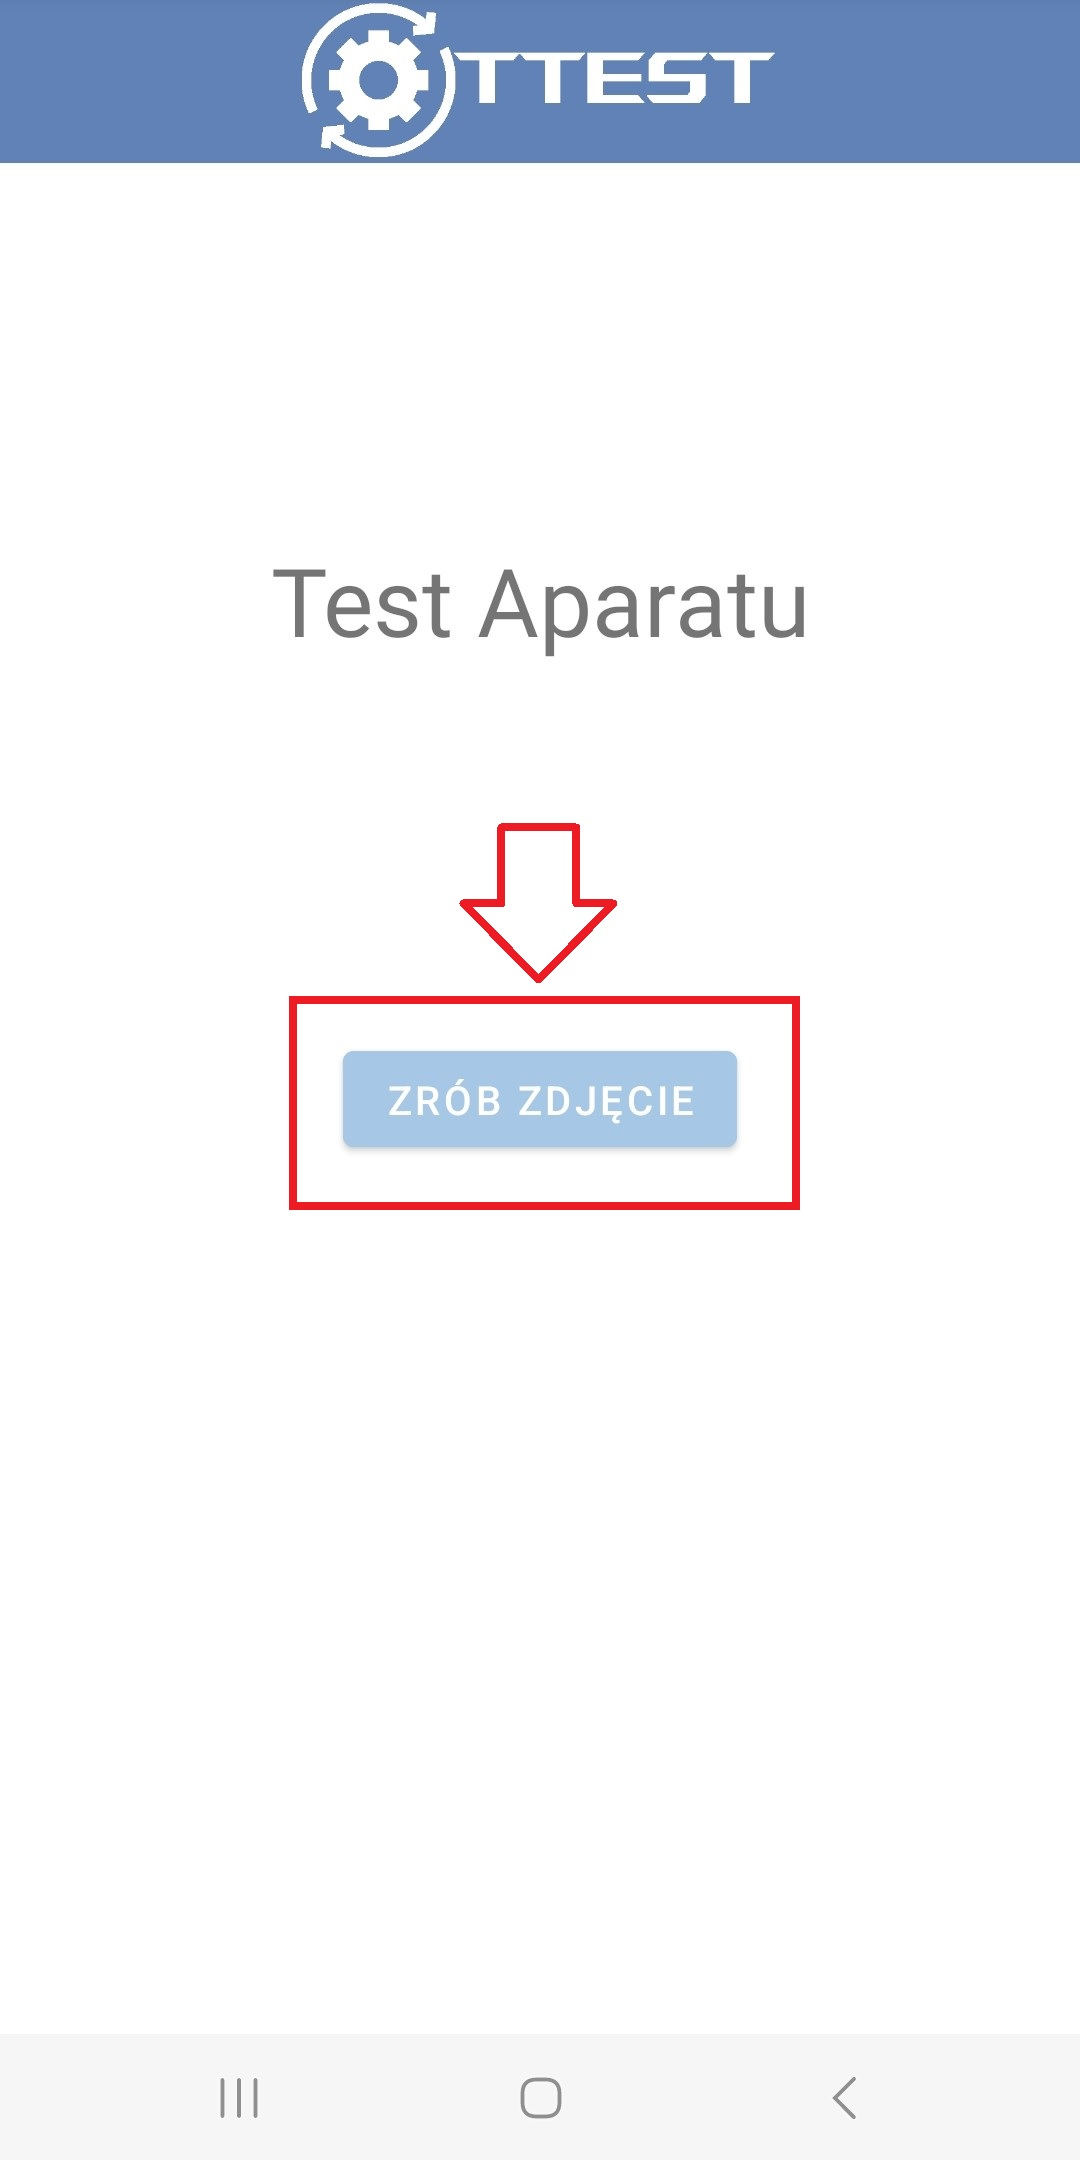
\includegraphics[angle=360, width=0.45\textwidth]{rys/punkt6/aparat}
		\caption{Strona testowa aparatu}
		\label{rys:aparat}
	\end{center}
\end{figure}

\newpage


Gdy naciśniemy przycisk zostaje uruchomiony aparat i możemy wykonać zdjęcie poprzez kliknięcie białego kółka znajdującego się u dołu ekranu.
Rysunek \ref{rys:aparat1} prezentuję test aparatu.

\begin{figure}[!hbt]
	\begin{center}
		
\includegraphics[angle=360, width=0.45\textwidth]{rys/punkt6/aparat1}
		\caption{Wykonanie zdjęcia- test aparatu}
		\label{rys:aparat1}
	\end{center}
\end{figure}

\newpage


Po wykonaniu zdjęcia, możemy ponowić próbę lub zakończyć test klikając przycisk: "OK". Rysunek \ref{rys:aparat2} przedstawia zrzut ekranu potwierdzający pomyślny przebieg testu.

\begin{figure}[!hbt]
	\begin{center}
		
\includegraphics[angle=360, width=0.45\textwidth]{rys/punkt6/aparat2}
		\caption{Wykonanie kolejnego zdjęcia lub koniec testu - test aparatu}
		\label{rys:aparat2}
	\end{center}
\end{figure}

\newpage


\subsection{Podsumowanie wszystkich testów}

\hspace{0.60cm}Aby przejść do wykonania podsumowania wszystkich testów, należy w menu głównym wybrać i kliknąć przycisk: "Wyniki" znajdujący się na samym dole pod wszystkimi testami. Rysunek \ref{rys:menu8} przedstawia miejsce które należy wybrać aby przejść do "Wyników".

\begin{figure}[!hbt]
	\begin{center}
		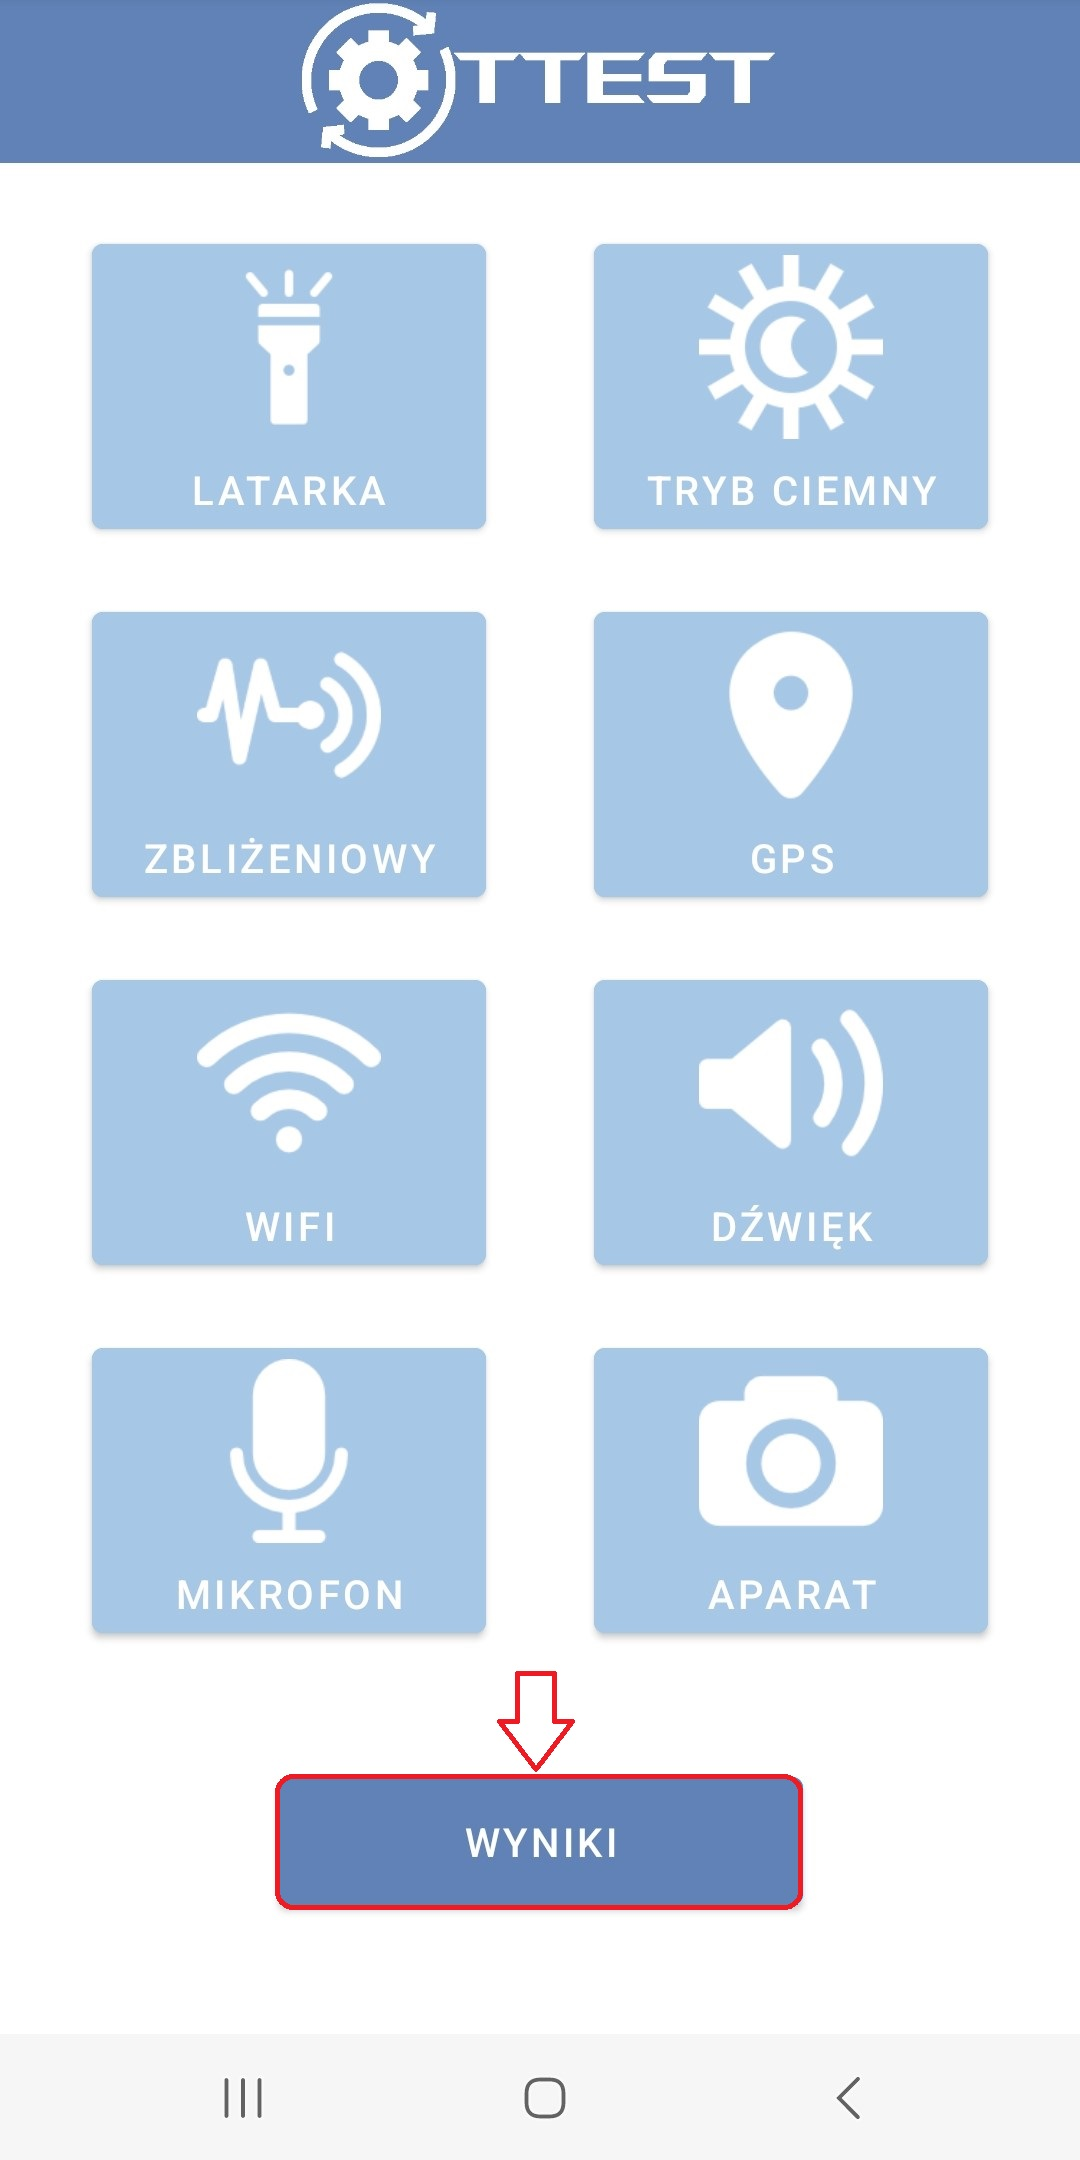
\includegraphics[angle=360, width=0.45\textwidth]{rys/punkt6/menu8}
		\caption{Przejście do sekcji "Wyniki"}
		\label{rys:menu8}
	\end{center}
\end{figure}

\newpage


Po przejściu na stronę z wynikami dostrzegamy że na samej górze po lewej stronie podany jest marka oraz model naszego telefonu. Co więcej na środku wymienione zostały wszystkie testy, które aplikacja posiada. Naszym zadaniem jest zaznaczyć odpowiednią odpowiedź w zależności czy test odbył się pomyślnie - odpowiedź "Tak" lub w przypadku gdy test nie przeszedł pomyślnie - odpowiedź "Nie". Następnym krokiem jest naciśnięcie przycisku "Podsumuj", który zsumuje wszystkie testy. Rysunek \ref{rys:wyniki} prezentuję podsumowanie testów.

\begin{figure}[!hbt]
	\begin{center}
		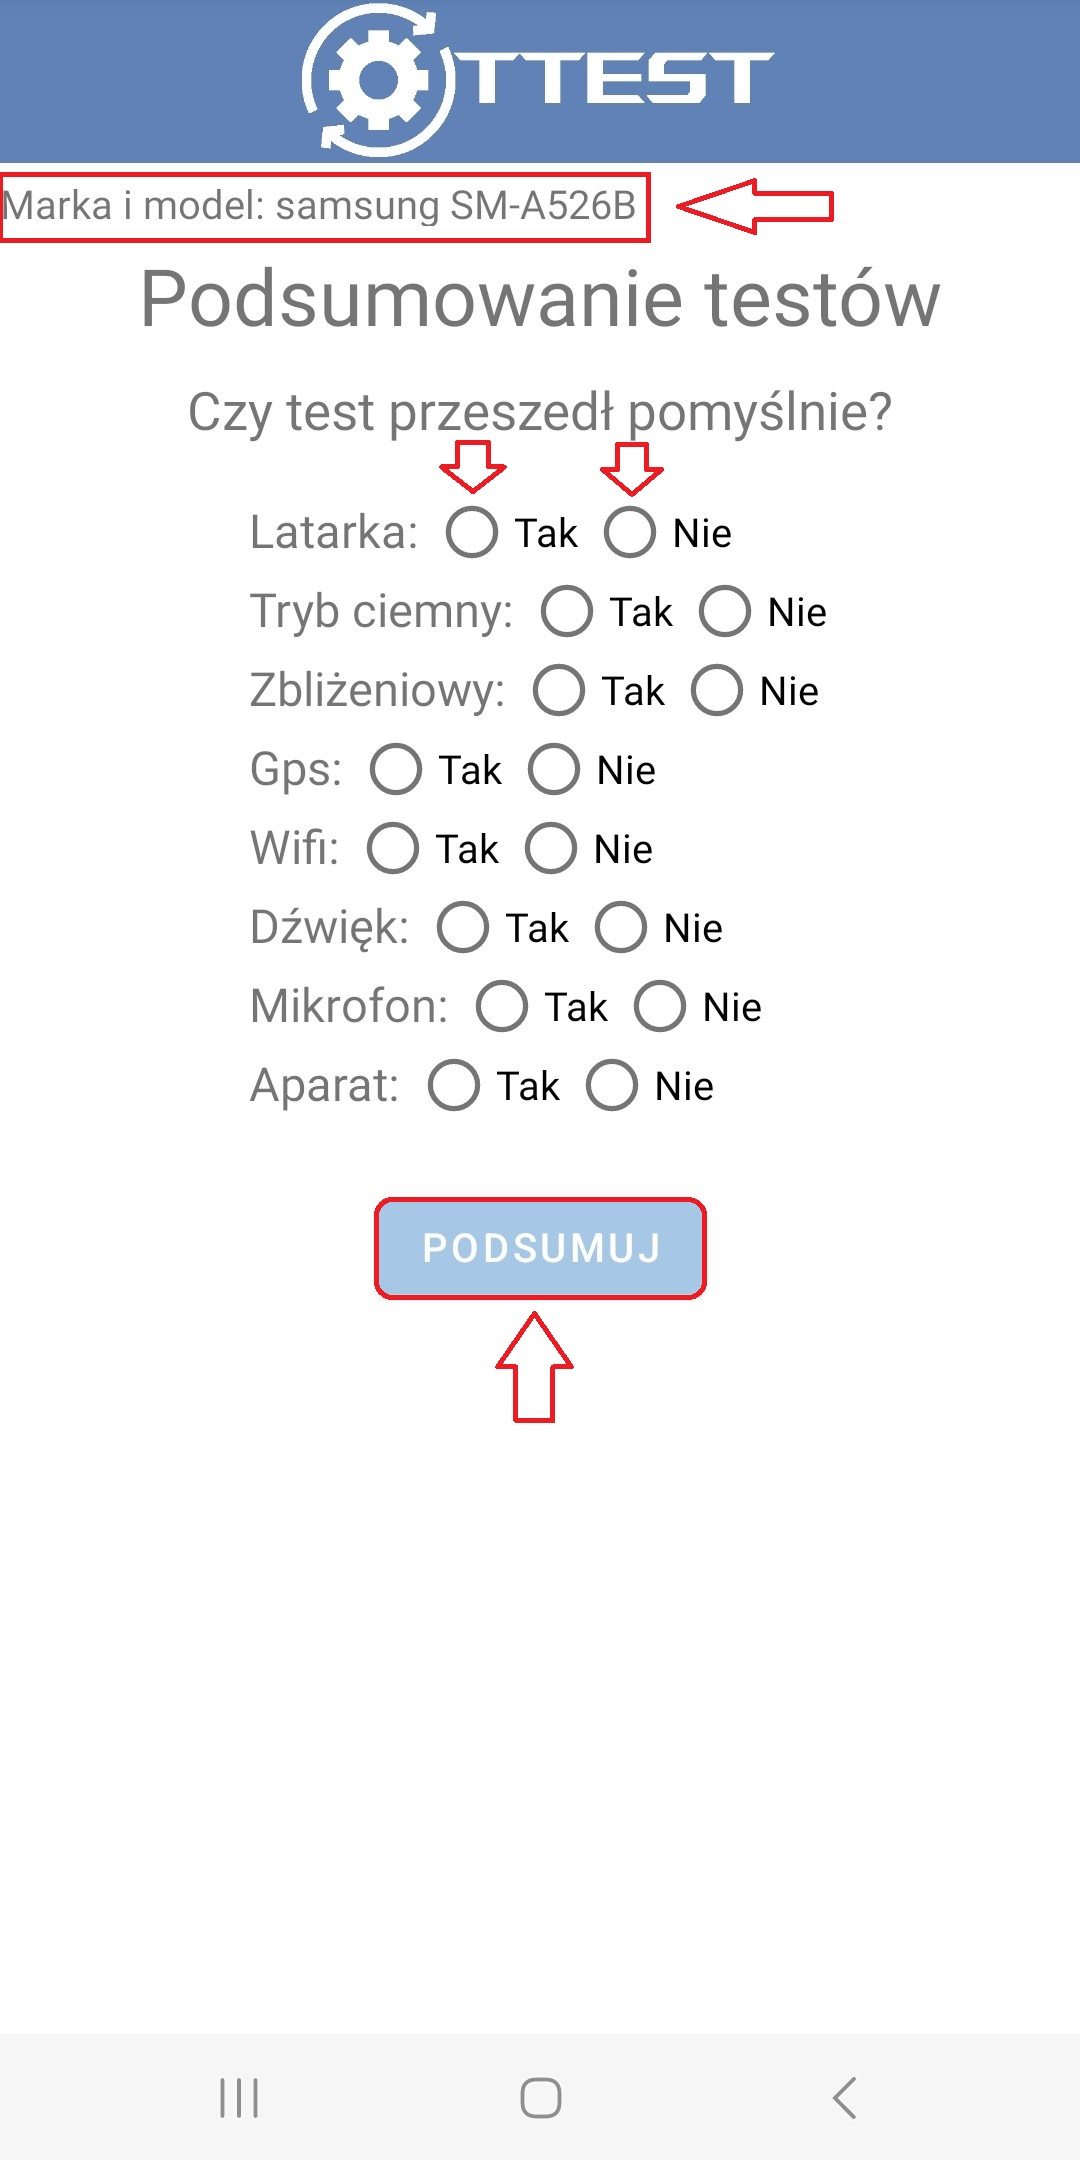
\includegraphics[angle=360, width=0.48\textwidth]{rys/punkt6/wyniki}
		\caption{Strona z podsumowaniem testów.}
		\label{rys:wyniki}
	\end{center}
\end{figure}

W przypadku gdy wszystkie testy przebiegły pomyślnie zostaną one wypisane zieloną czcionką, u dołu ekranu pod przyciskiem podsumowującym. Rysunek \ref{rys:wyniki1} prezentuję podsumowanie wszystkich testów, które przebiegły pomyślnie.

\newpage


\begin{figure}[!hbt]
	\begin{center}
		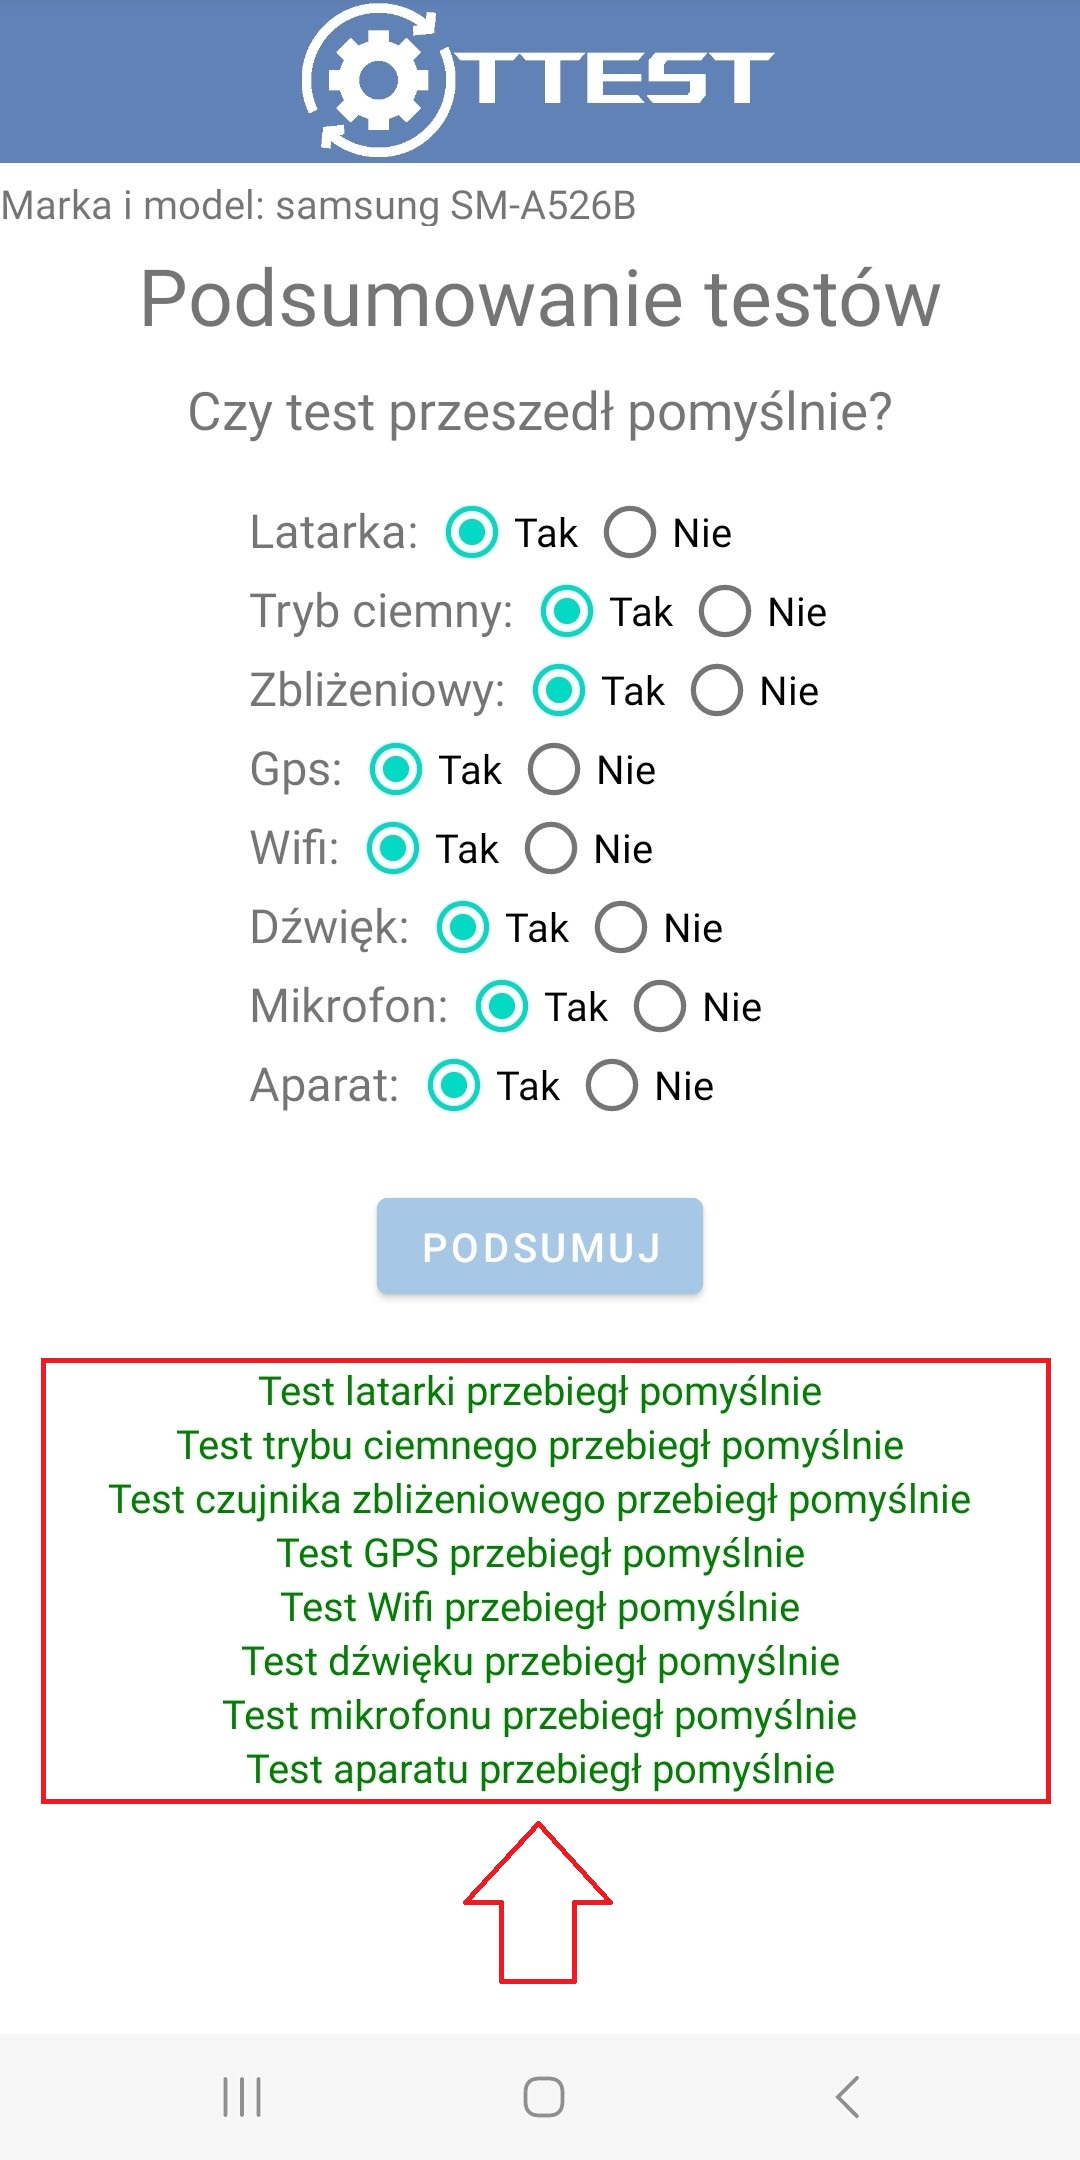
\includegraphics[angle=360, width=0.31\textwidth]{rys/punkt6/wyniki1}
		\caption{Podsumowanie wszystkich testów, które przebiegły pomyślnie}
		\label{rys:wyniki1}
	\end{center}
\end{figure}

Jeżeli wszystkie testy nie przebiegły pomyślnie zostaną one wypisane czerwoną czcionką, u dołu ekranu pod przyciskiem podsumowującym. Rysunek \ref{rys:wyniki2} prezentuję podsumowanie wszystkich testów, które nie przebiegły pomyślnie.

\begin{figure}[!hbt]
	\begin{center}
		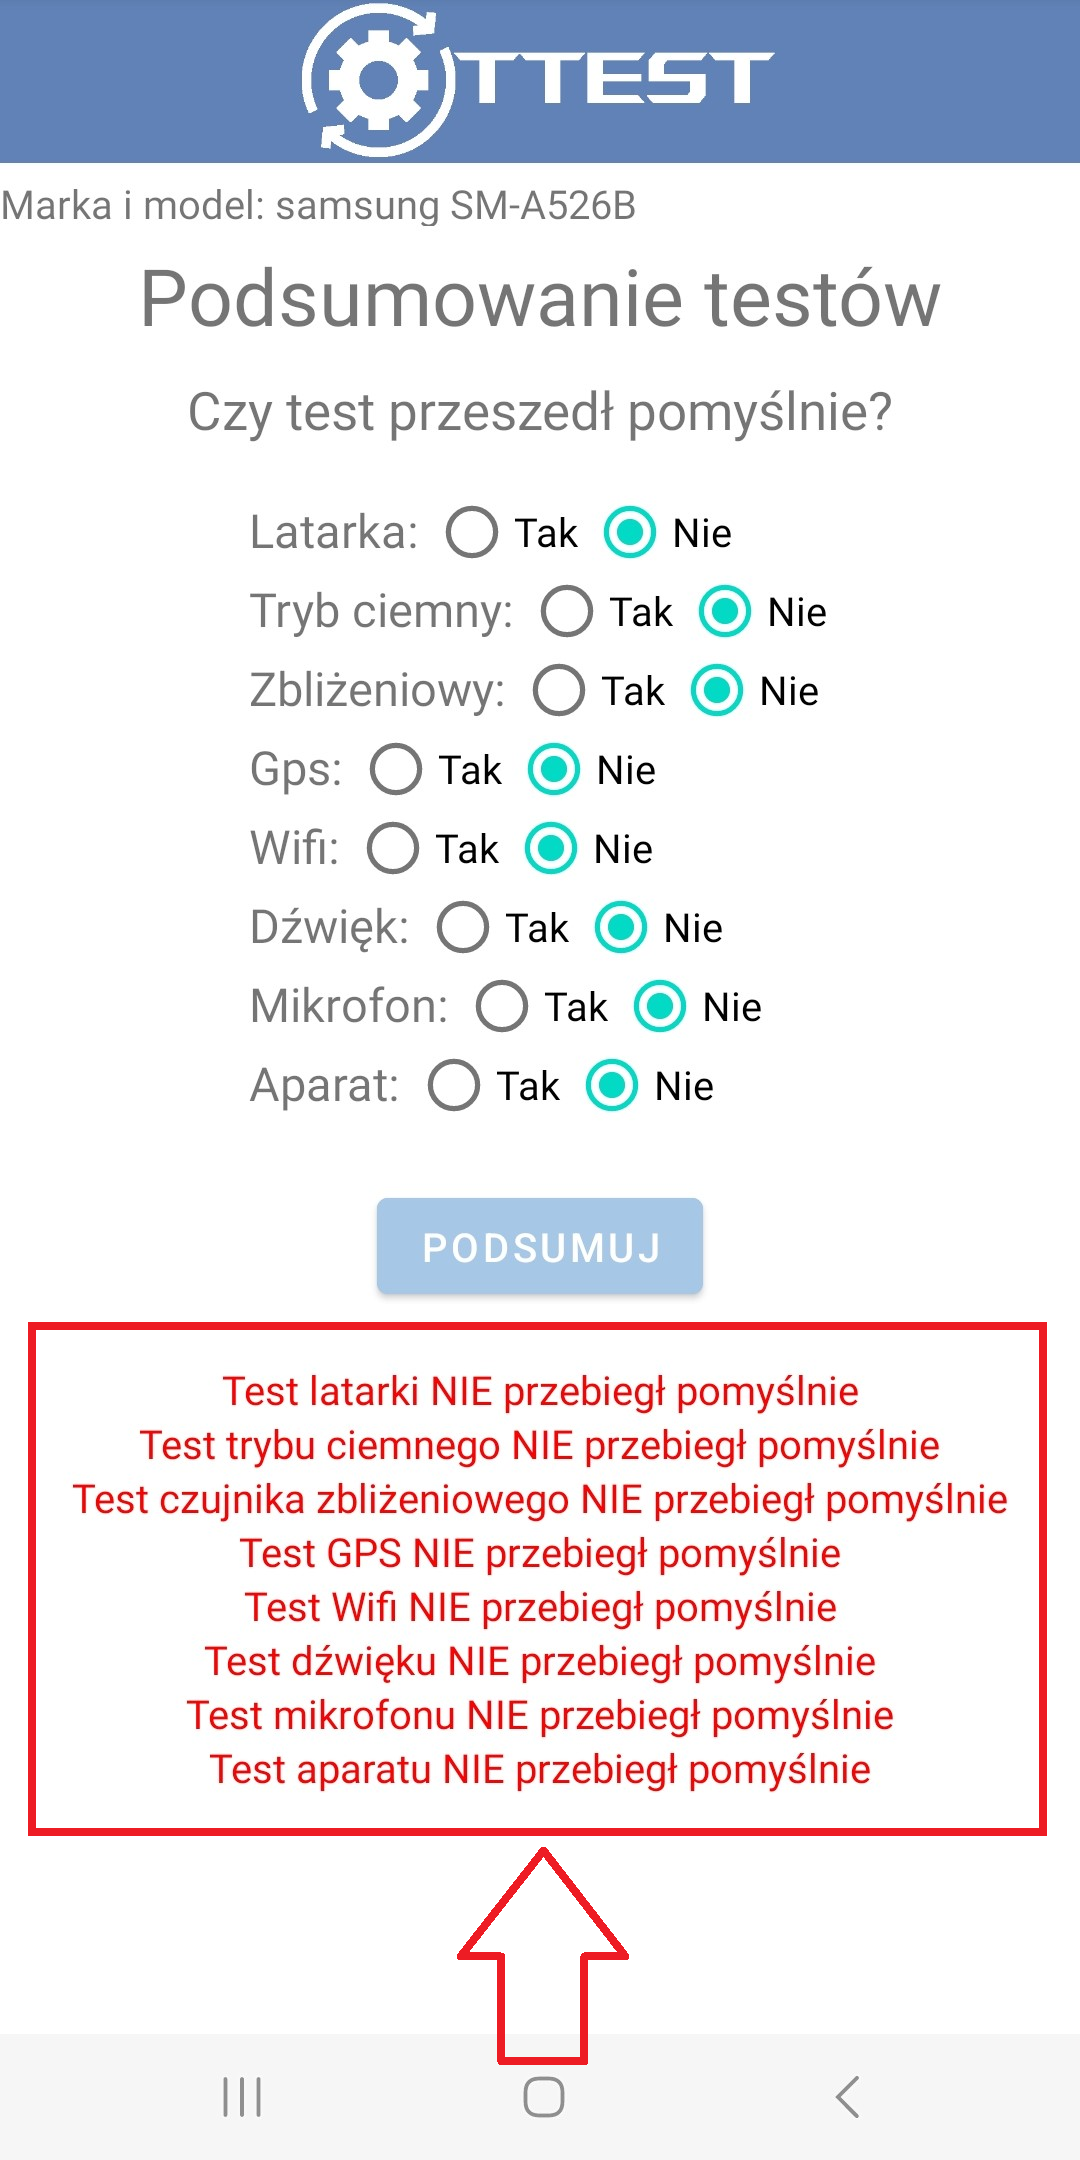
\includegraphics[angle=360, width=0.31\textwidth]{rys/punkt6/wyniki2}
		\caption{Podsumowanie wszystkich testów, które nie przebiegły pomyślnie}
		\label{rys:wyniki2}
	\end{center}
\end{figure}













       
%%%%%%%%%%%%%%%%%%% koniec treść główna dokumentu %%%%%%%%%%%%%%%%%%%%%
	\newpage
    \addcontentsline{toc}{section}{Literatura}  
	\printbibliography

    \newpage
    \hypersetup{linkcolor=black}
    \renewcommand{\cftparskip}{3pt}
    \clearpage
    \renewcommand{\cftloftitlefont}{\Large\bfseries\sffamily}
    \listoffigures
    \addcontentsline{toc}{section}{Spis rysunków}
	\thispagestyle{fancy}
	
    \newpage
    \renewcommand{\cftlottitlefont}{\Large\bfseries\sffamily}
    \def\listtablename{Spis tabel}
    \addcontentsline{toc}{section}{Spis tabel}\listoftables 
	\thispagestyle{fancy}
	
	\newpage
	\renewcommand{\cftlottitlefont}{\Large\bfseries\sffamily}
	\renewcommand\lstlistlistingname{Spis listingów}
	\addcontentsline{toc}{section}{Spis listingów}\lstlistoflistings 
	\thispagestyle{fancy}
	


    %lista rzeczy do zrobienia: wypisuje na koñcu dokumentu, patrz: pakiet todo.sty
    \todos
    %koniec listy rzeczy do zrobienia
\end{document}
